\section{Background Rejection}\label{sec:bkg}
In this section we will describe the cuts we could apply to our selected events, in order to isolate the $\nu_{e}$ CC$0\pi$-Np event candidates. The cuts have been chosen to (1) reduce the background, and (2) ensure that the selected events are well reconstructed. The values of each cut have been chosen manually to maximise the purity while retaining a sufficient efficiency. %It would have been possible, in theory, to calculate an optimal set of cuts, maximized by the significance of the $\nu_{e}$ CC0$\pi$-Np events. However, this set of cuts would not have allowed a correct validation of the final selected sample, due to the limited size of the data unblinded sample. As such, the chosen cuts increase the purity of our sample, but also retain a significant amount ($\approx 20$) of selected data events.


\subsection{Rectangular cuts}\label{sec:cuts}
The goal of the rectangular cuts is to isolate the $\nu_e$ CC0$\pi$-Np events and increase the purity of our selected sample. However, in order to validate our cuts and verify the agreement between data and Monte Carlo also after this stage, it is necessary to select also a sufficient number of data events. In particular, in this analysis we require at least one data event in the bins in the $[0.2,1.9]$~GeV range of the $E_{\mathrm{deposited}}$ spectrum, which is also the energy region we are most interested into. 

In this section we will study all the variables used to apply the kinematic and calorimetric cuts. In particular, we will show, for each variable:
\begin{itemize}
\item the area-normalised Monte Carlo distributions for the signal ($\nu_{e}$ CC0$\pi$-Np events), the cosmogenic background (cosmic, cosmic contaminated, and cosmic in-time), and the neutrino background ($\nu_{e}$ CC, beam intrinsic $\nu_{\mu}$, beam intrinsic NC, and outside fid. vol.), to show the rejection power of each cut;
\item the POT-normalised Monte Carlo and data distributions, to verify the agreement of the simulation with the collected data, categorised according to the event type.
\item for shower and track variables, the POT-normalised Monte Carlo and data distributions, categorised according to the particle type.
\end{itemize}

\subsubsection*{Number of reconstructed hits $> 50$} 
A large number of cosmic-ray events may fake a neutrino candidate with a low number of hits. Thus, we require at least 50 reconstructed hits in the three wire planes to reduce this cosmogenic background. 
%This happens because the reconstruction framework is not always able to identify delta rays and Michel electrons as byproducts of the cosmic ray. We then require at least 50 reconstructed hits in order to reduce this background. 
The area-normalised distributions in Figure \ref{fig:nhits_integral} show that a large fraction of the cosmogenic backgrounds has a very low number of reconstructed hits in the collection plane, while the signal and the neutrino components have a much broader distribution. Figure \ref{fig:nhits_pot} shows a good data/Monte Carlo agreement for this variable.

\begin{figure}[htbp]
\centering
  \begin{subfigure}{0.49\textwidth}
    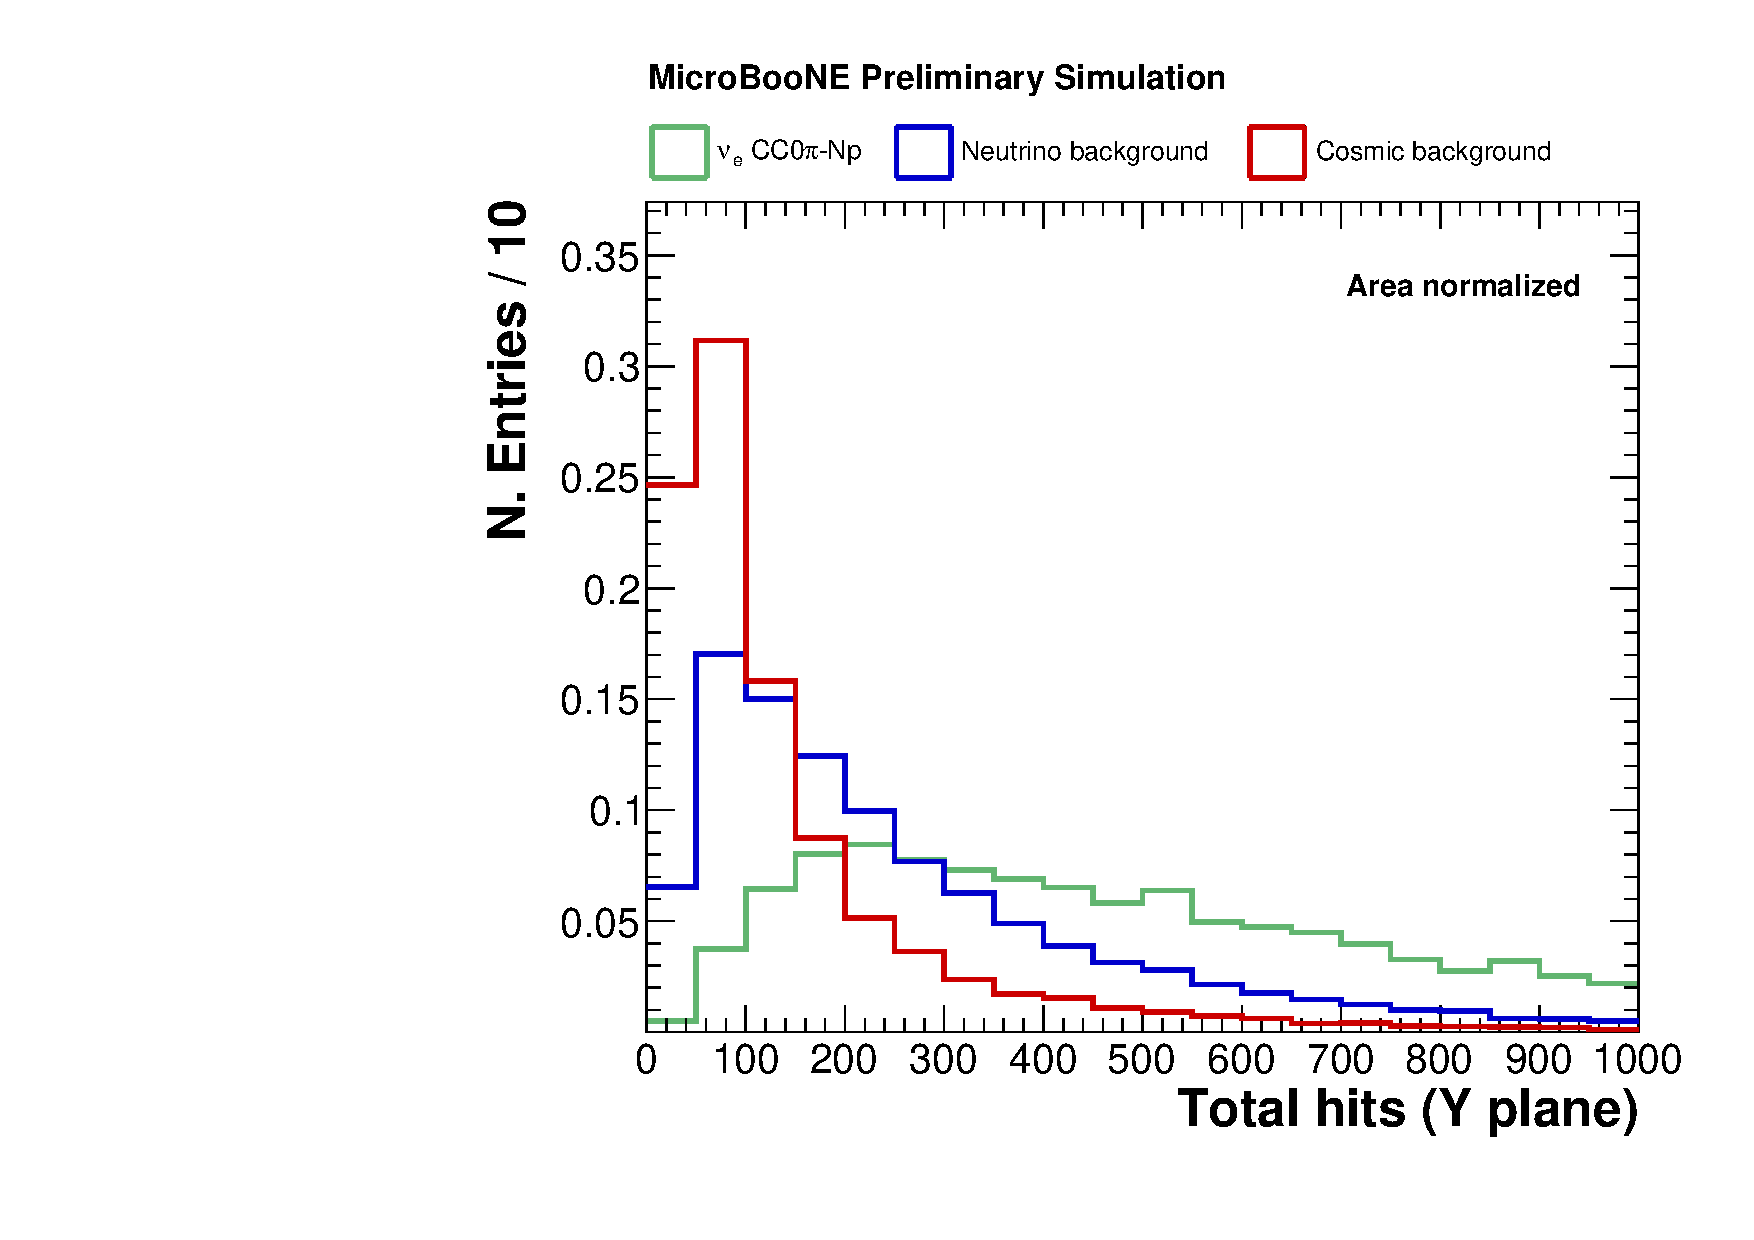
\includegraphics[width=\linewidth]{figures/h_total_hits_y_norm.pdf}
    \caption{Area-normalised.} \label{fig:nhits_integral}
  \end{subfigure}
    \begin{subfigure}{0.49\textwidth}
    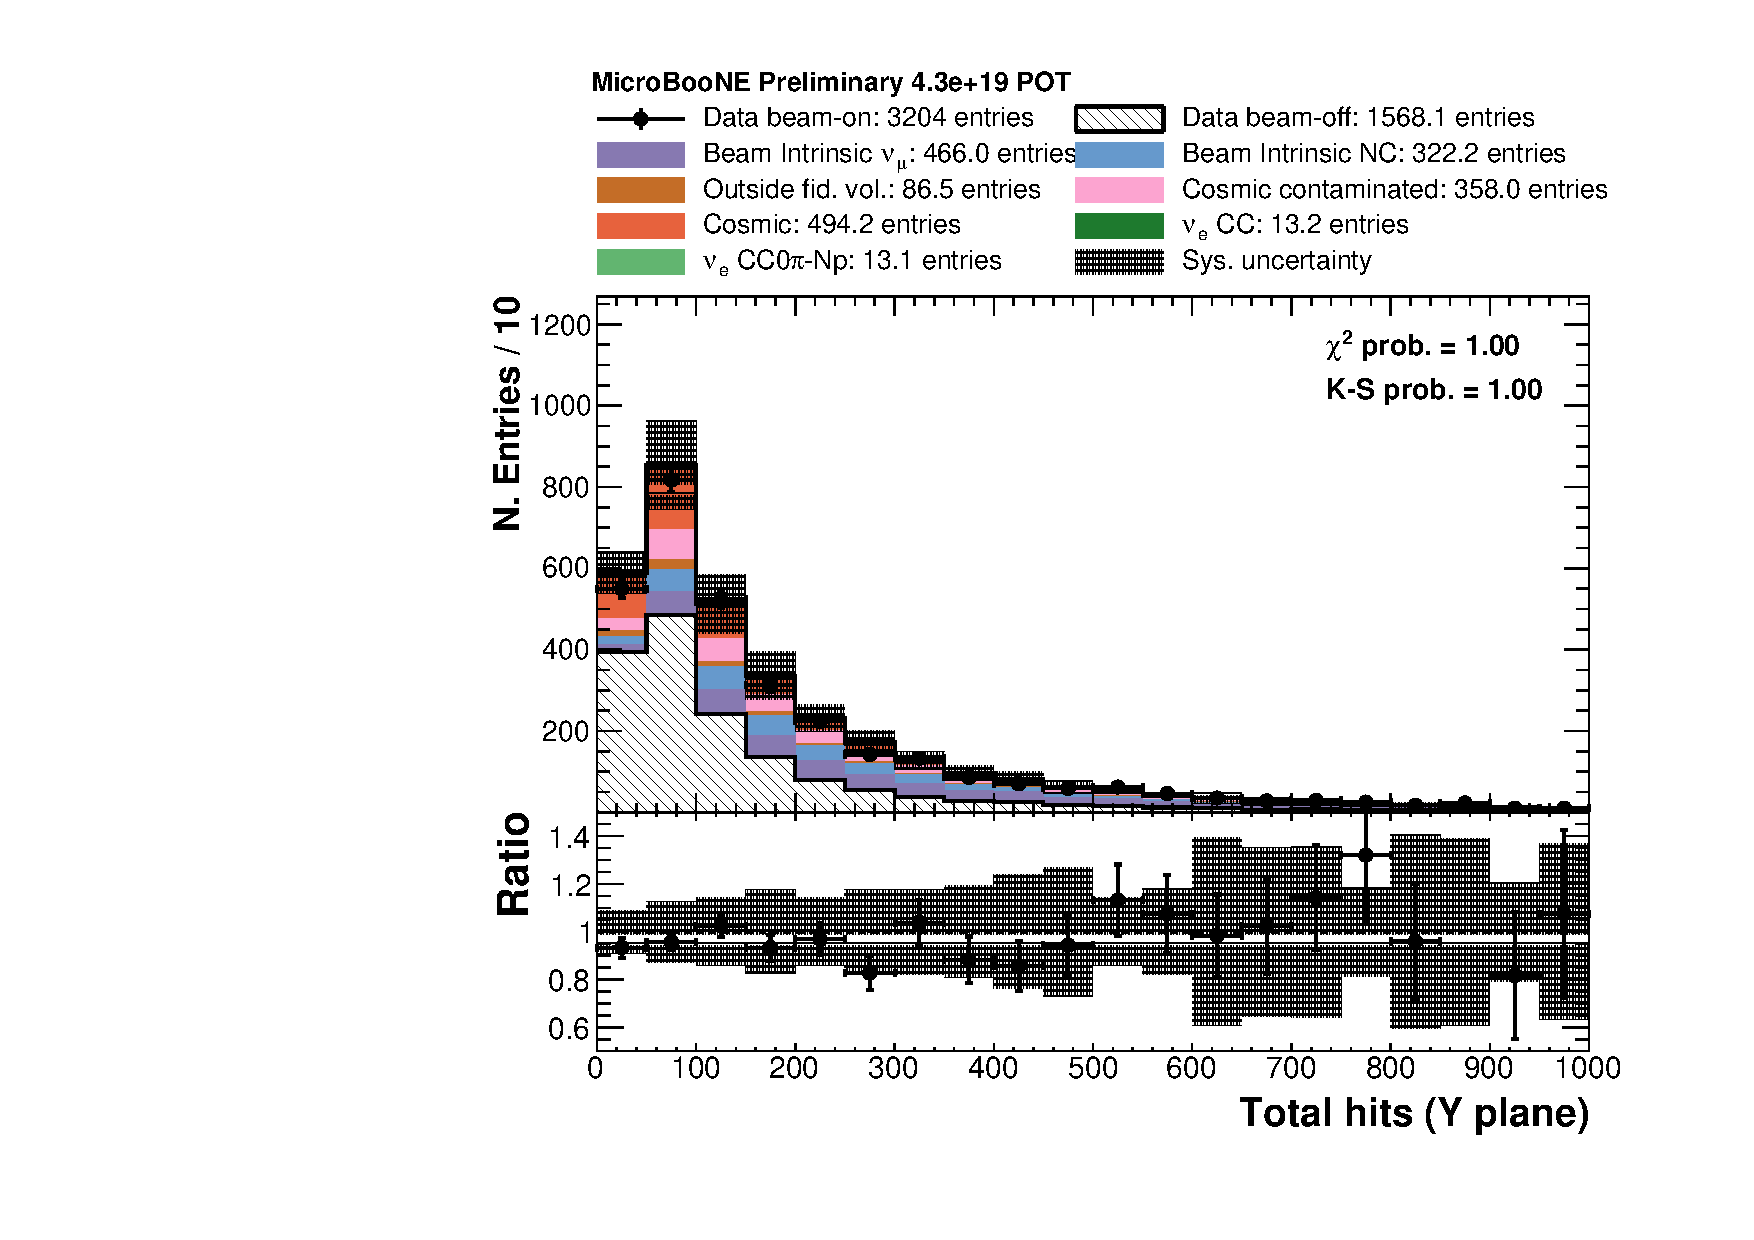
\includegraphics[width=\linewidth]{figures/h_total_hits_y.pdf}
    \caption{POT-normalised.} \label{fig:nhits_pot}
  \end{subfigure}
  \caption{Area and POT-normalised distributions of the number of reconstructed hits in the collection plane for all the objects in the event.}
\end{figure}


\subsubsection*{Fraction of shower hits $> 0.5$}
Cosmic-ray and CC $\nu_{\mu}$ events faking a $\nu_{e}$ CC0$\pi$-Np candidate will have in general a long muon track and a small Michel electron at the end. In these cases, the hits associated to the reconstructed showers will represent a small fraction of the total number of hits, as shown in Figure \ref{fig:ratio_norm}. Signal events, on the contrary, have a large fraction of hits associated to shower objects. We require the ratio between the number of shower hits and track hits to be larger than 0.5. Figure \ref{fig:ratio_pot} shows the agreement between data and Monte Carlo for this quantity.

\begin{figure}[htbp]
\centering
  \begin{subfigure}{0.49\textwidth}
    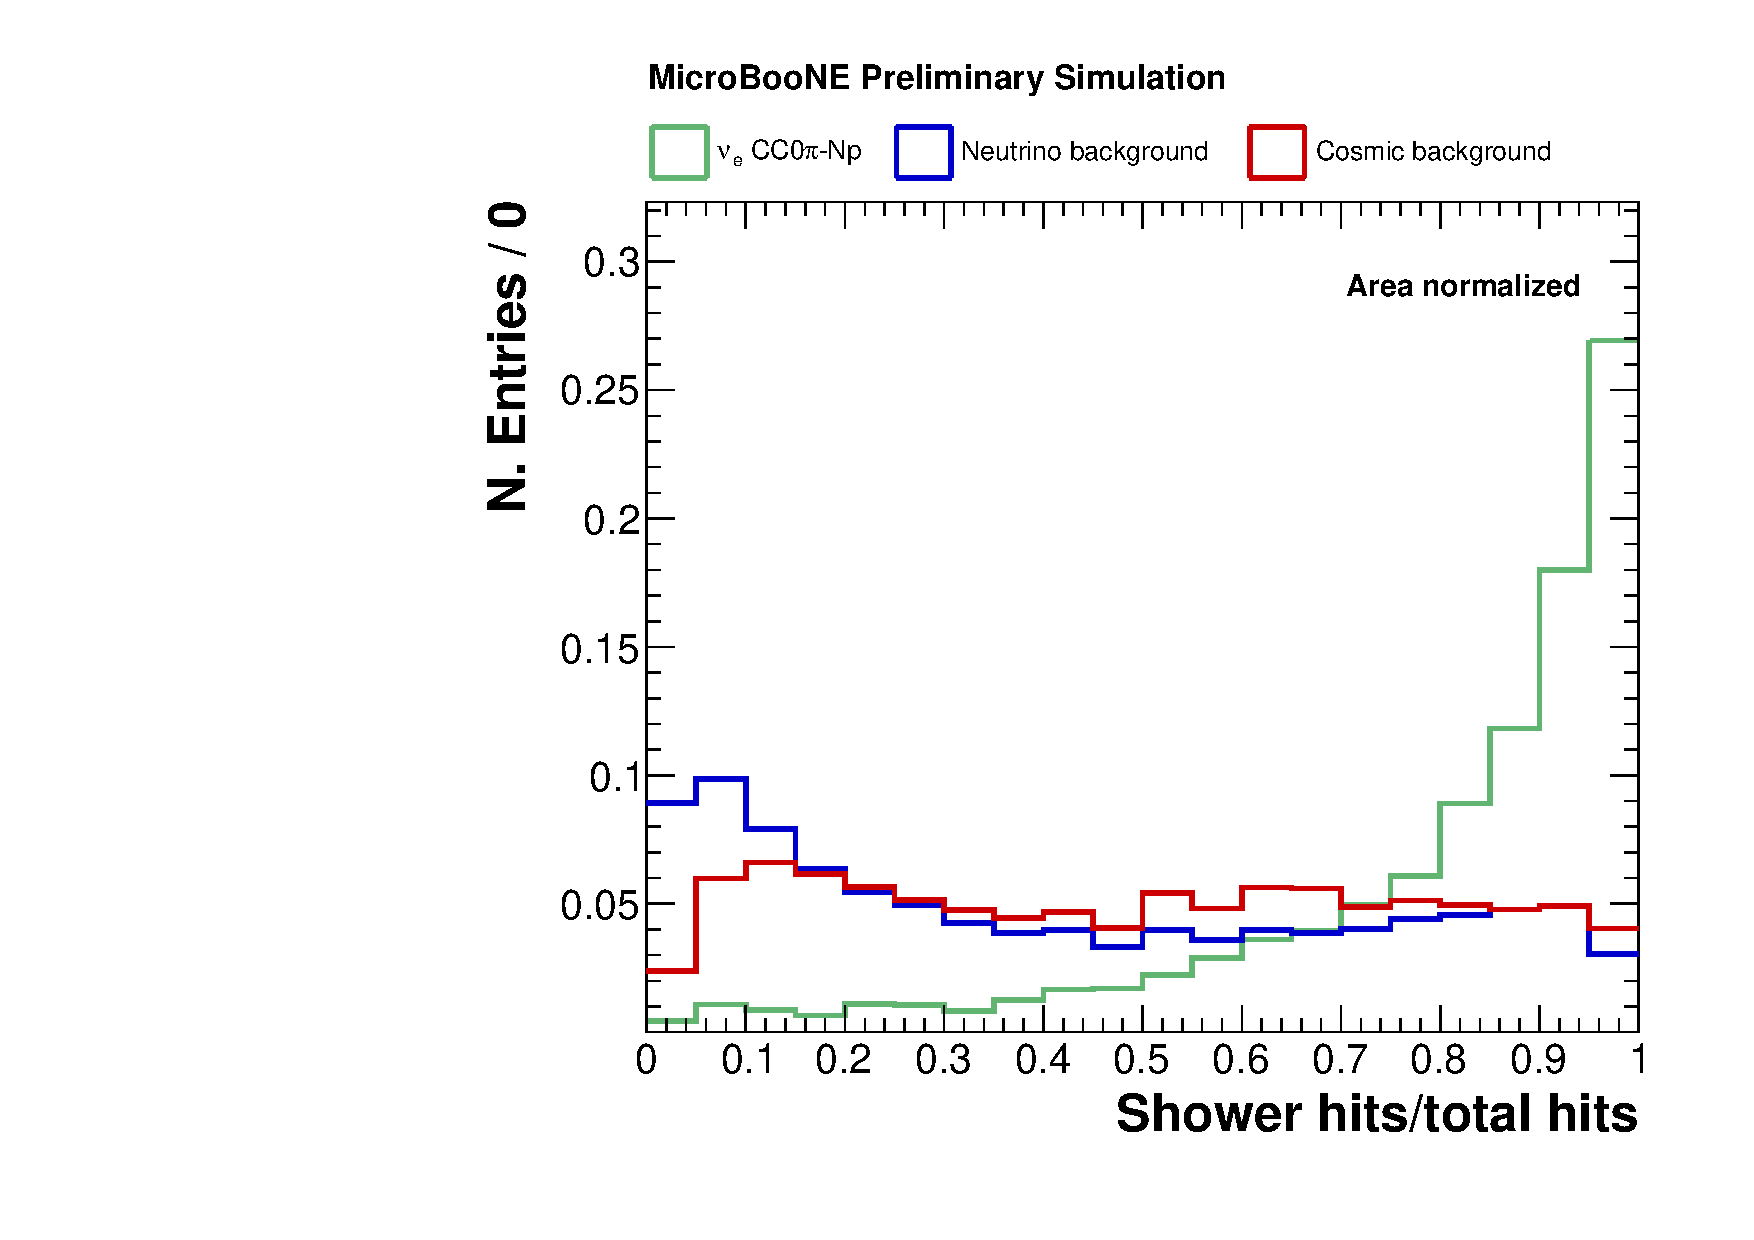
\includegraphics[width=\linewidth]{figures/h_hits_ratio_norm.pdf}
    \caption{Area-normalised.} \label{fig:ratio_norm}
  \end{subfigure}
    \begin{subfigure}{0.49\textwidth}
    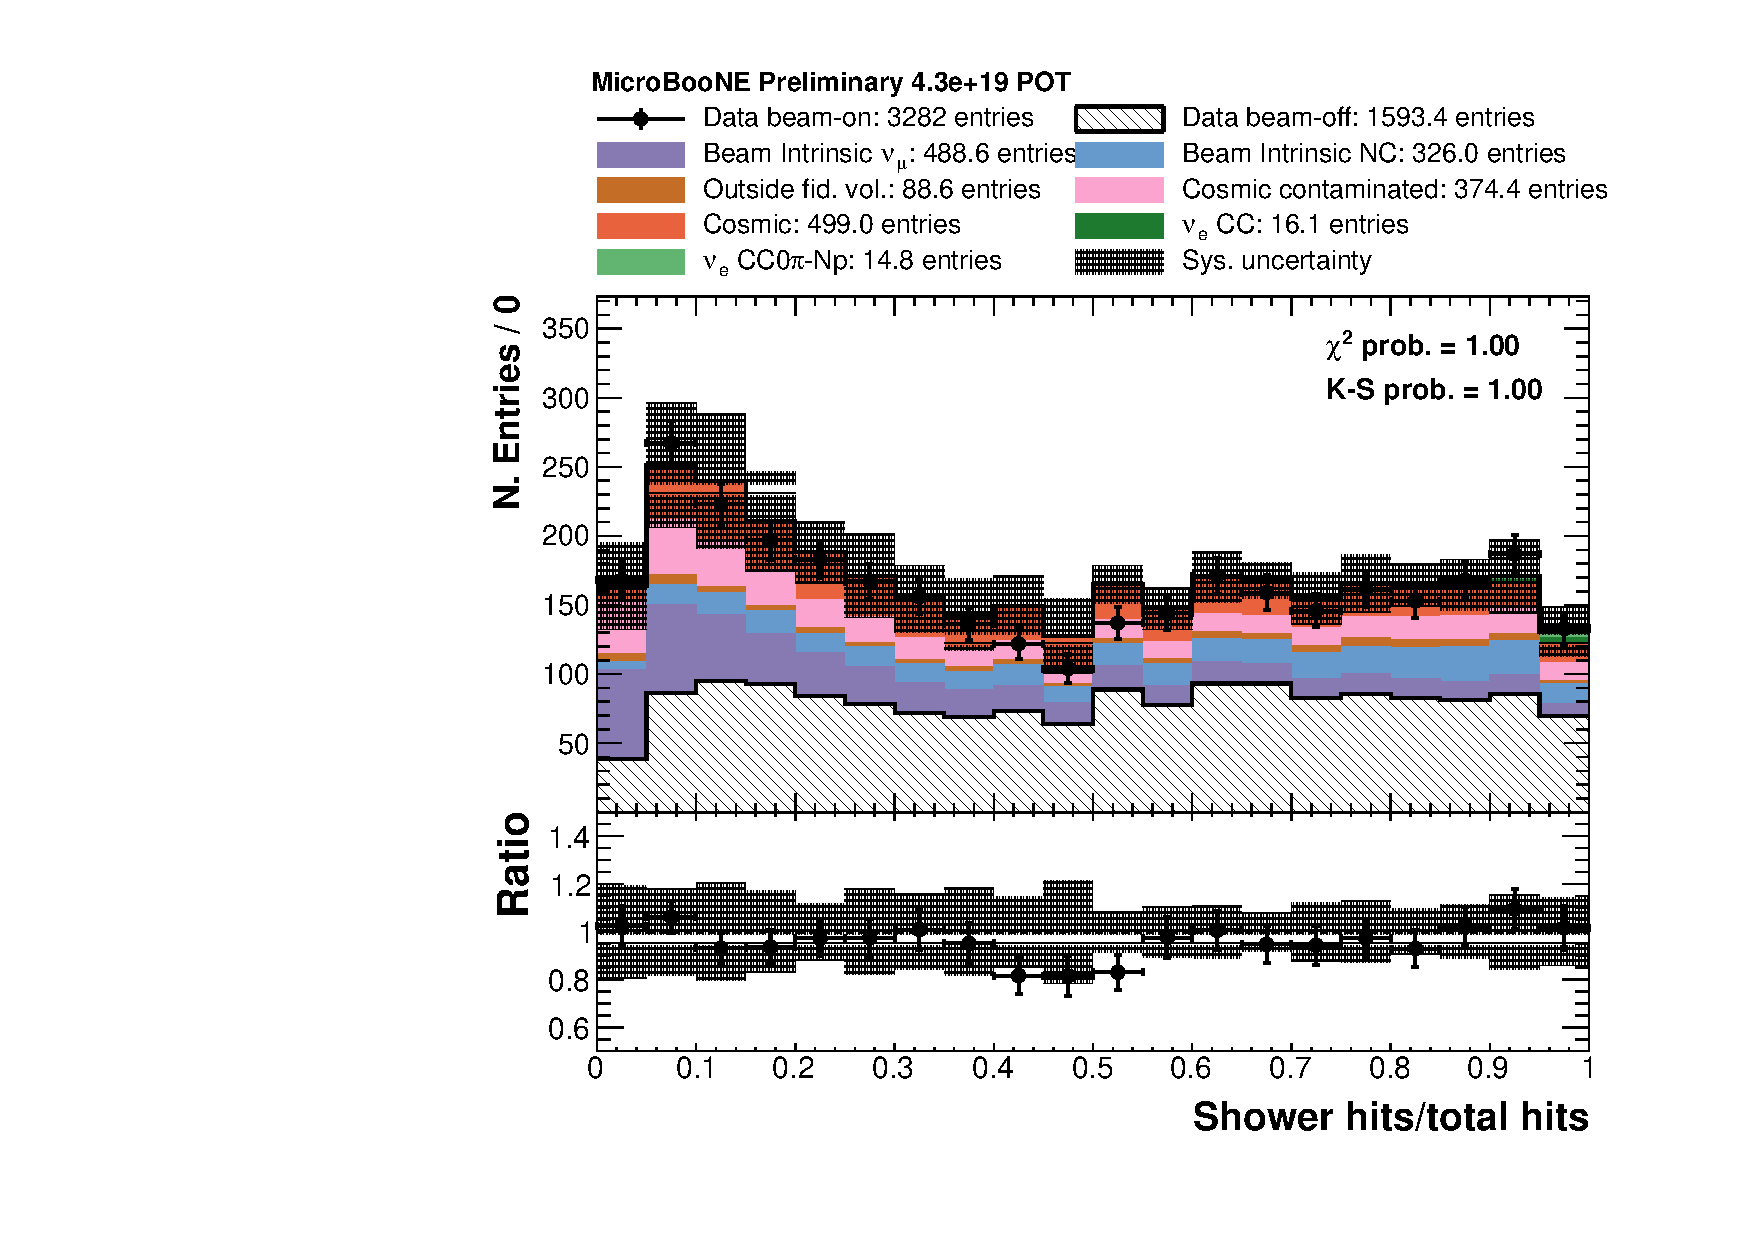
\includegraphics[width=\linewidth]{figures/h_hits_ratio.pdf}
    \caption{POT-normalised.} \label{fig:ratio_pot}
  \end{subfigure}
  \caption{Area and POT-normalised distributions of the ratio between the hits associated to reconstructed showers and the total number of reconstructed hits in the collection plane.}
\end{figure}


\subsubsection*{Most energetic shower $1~\mathrm{MeV/cm} < dE/dx <3.2~\mathrm{MeV/cm}$}
Our signal will contain an electron shower, so we require the $dE/dx$ of the leading shower to be around the 2~MeV/cm peak.

Figure \ref{fig:dedx_norm} shows that the signal distribution is peaked around 2 MeV/cm, as expected. The beam intrinsic NC component has a second peak around 4 MeV/cm, mainly caused by $\pi^0\rightarrow2\gamma$ decays. 
Figure \ref{fig:dedx_pdg} shows that electromagnetic showers originated by photons have a peak around 4~MeV/cm, as expected, and a peak around 2~MeV/cm. 

The POT-normalised plots (Figure \ref{fig:dedx_pot}, \ref{fig:dedx_pdg}) show a good agreement between data and Monte Carlo.

\begin{figure}[htbp]
\centering
  \begin{subfigure}{0.49\textwidth}
    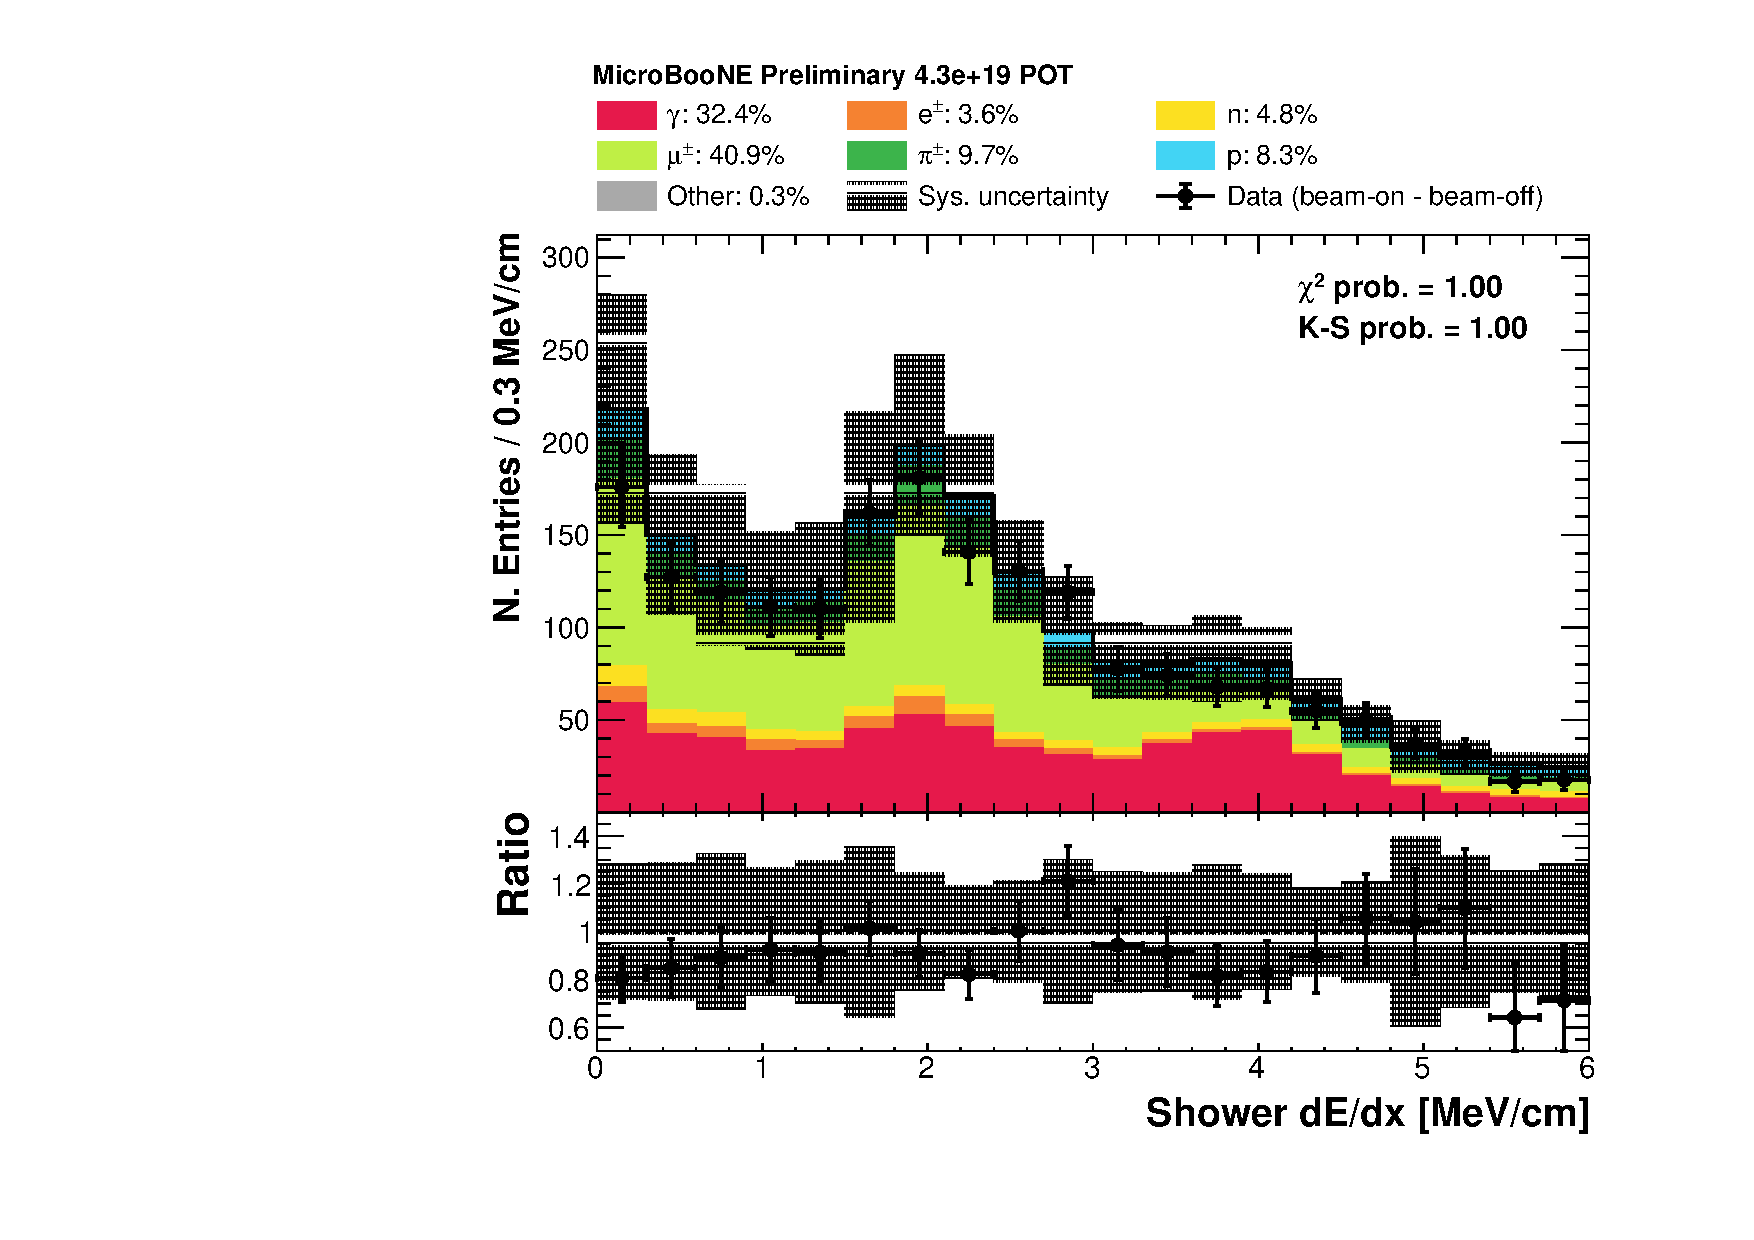
\includegraphics[width=\linewidth]{figures/h_shower_dedx_cali_pdg.pdf}
    \caption{POT-normalised, generating particle.} \label{fig:dedx_pdg}
  \end{subfigure}
  \begin{subfigure}{0.49\textwidth}
    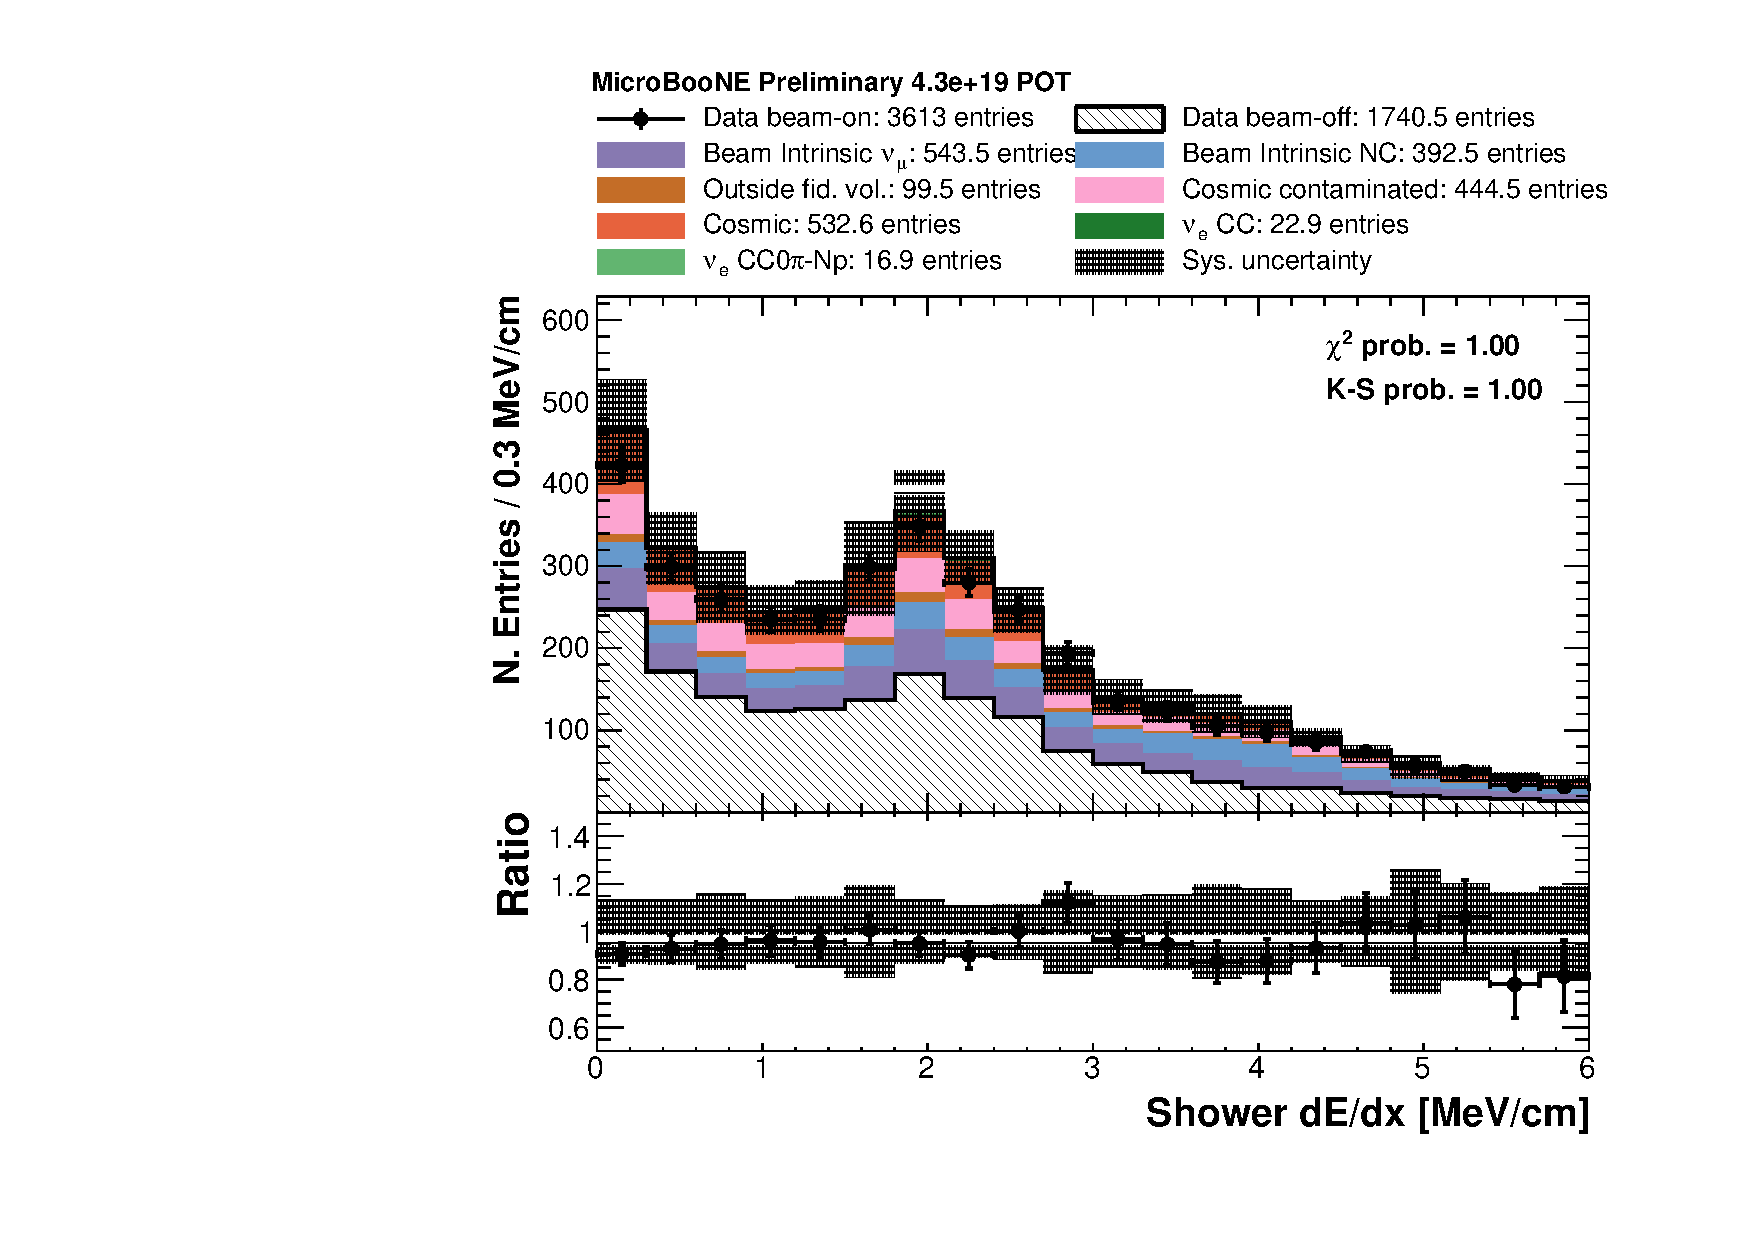
\includegraphics[width=\linewidth]{figures/h_shower_dedx_cali.pdf}
    \caption{POT-normalised, event category.} \label{fig:dedx_pot}
  \end{subfigure}
  \begin{subfigure}{0.49\textwidth}
    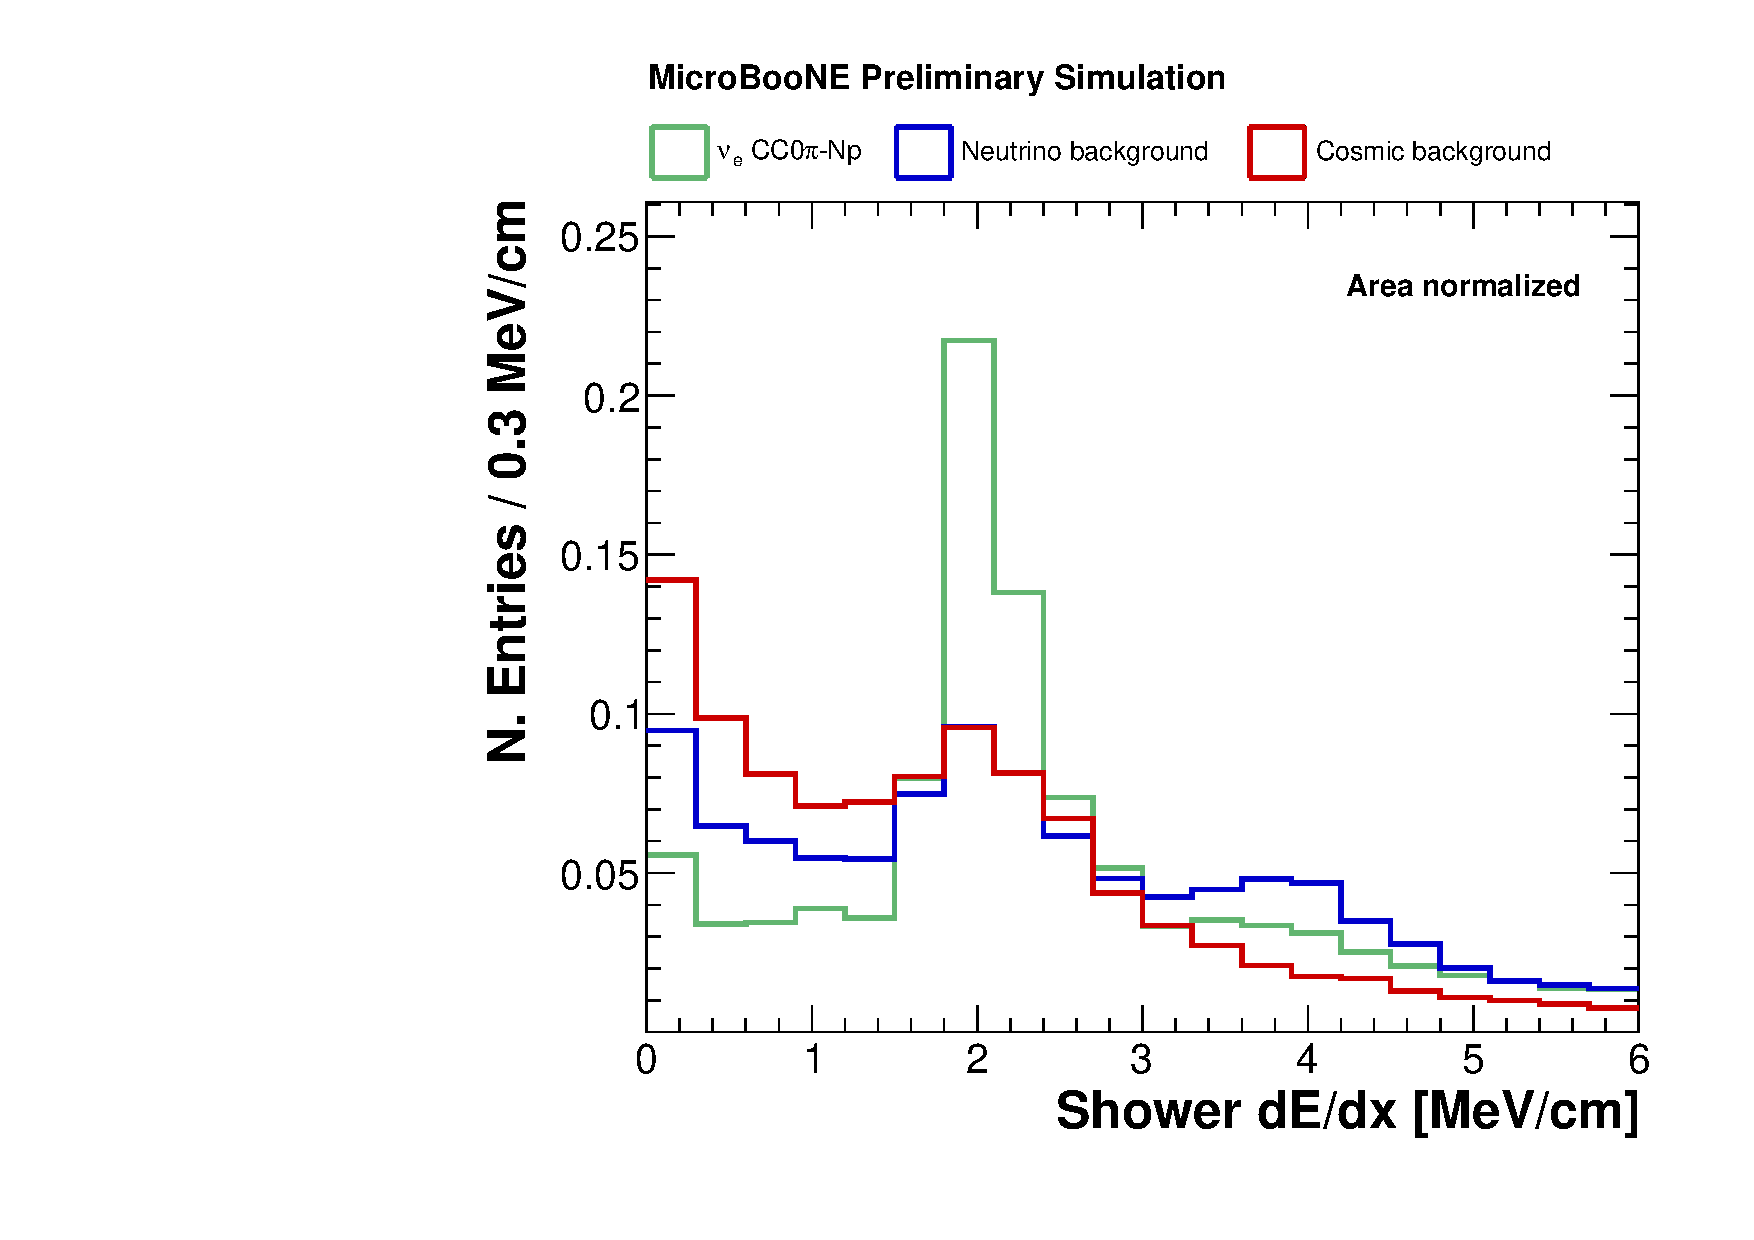
\includegraphics[width=\linewidth]{figures/h_shower_dedx_cali_norm.pdf}
    \caption{Area-normalised.} \label{fig:dedx_norm}
  \end{subfigure}
  \caption{Area and POT-normalised distributions of the $dE/dx$ of the reconstructed showers, classified according to the event category and to the primary particle generating the shower.}\label{fig:dedx_datamc}
\end{figure}

\subsubsection*{Track distance $d_{t} < 5$~cm}
A well reconstructed event with a proton in the final state will have a reconstructed track attached to the reconstructed neutrino vertex. This conservative cut can be tightened as understanding of the spatial resolution improves. The track with the lowest proton $\chi^2$ score is required to be within 5~cm of the reconstructed neutrino vertex.
Figure \ref{fig:trackd_norm} shows that the distributions of the distance between the start point of the reconstructed tracks and the reconstructed neutrino vertex for signal and background are very similar. The cut $d_{t} < 5$~cm, then, mainly ensures that the event is well reconstructed. 

\begin{figure}[htbp]
\centering
  \begin{subfigure}{0.49\textwidth}
    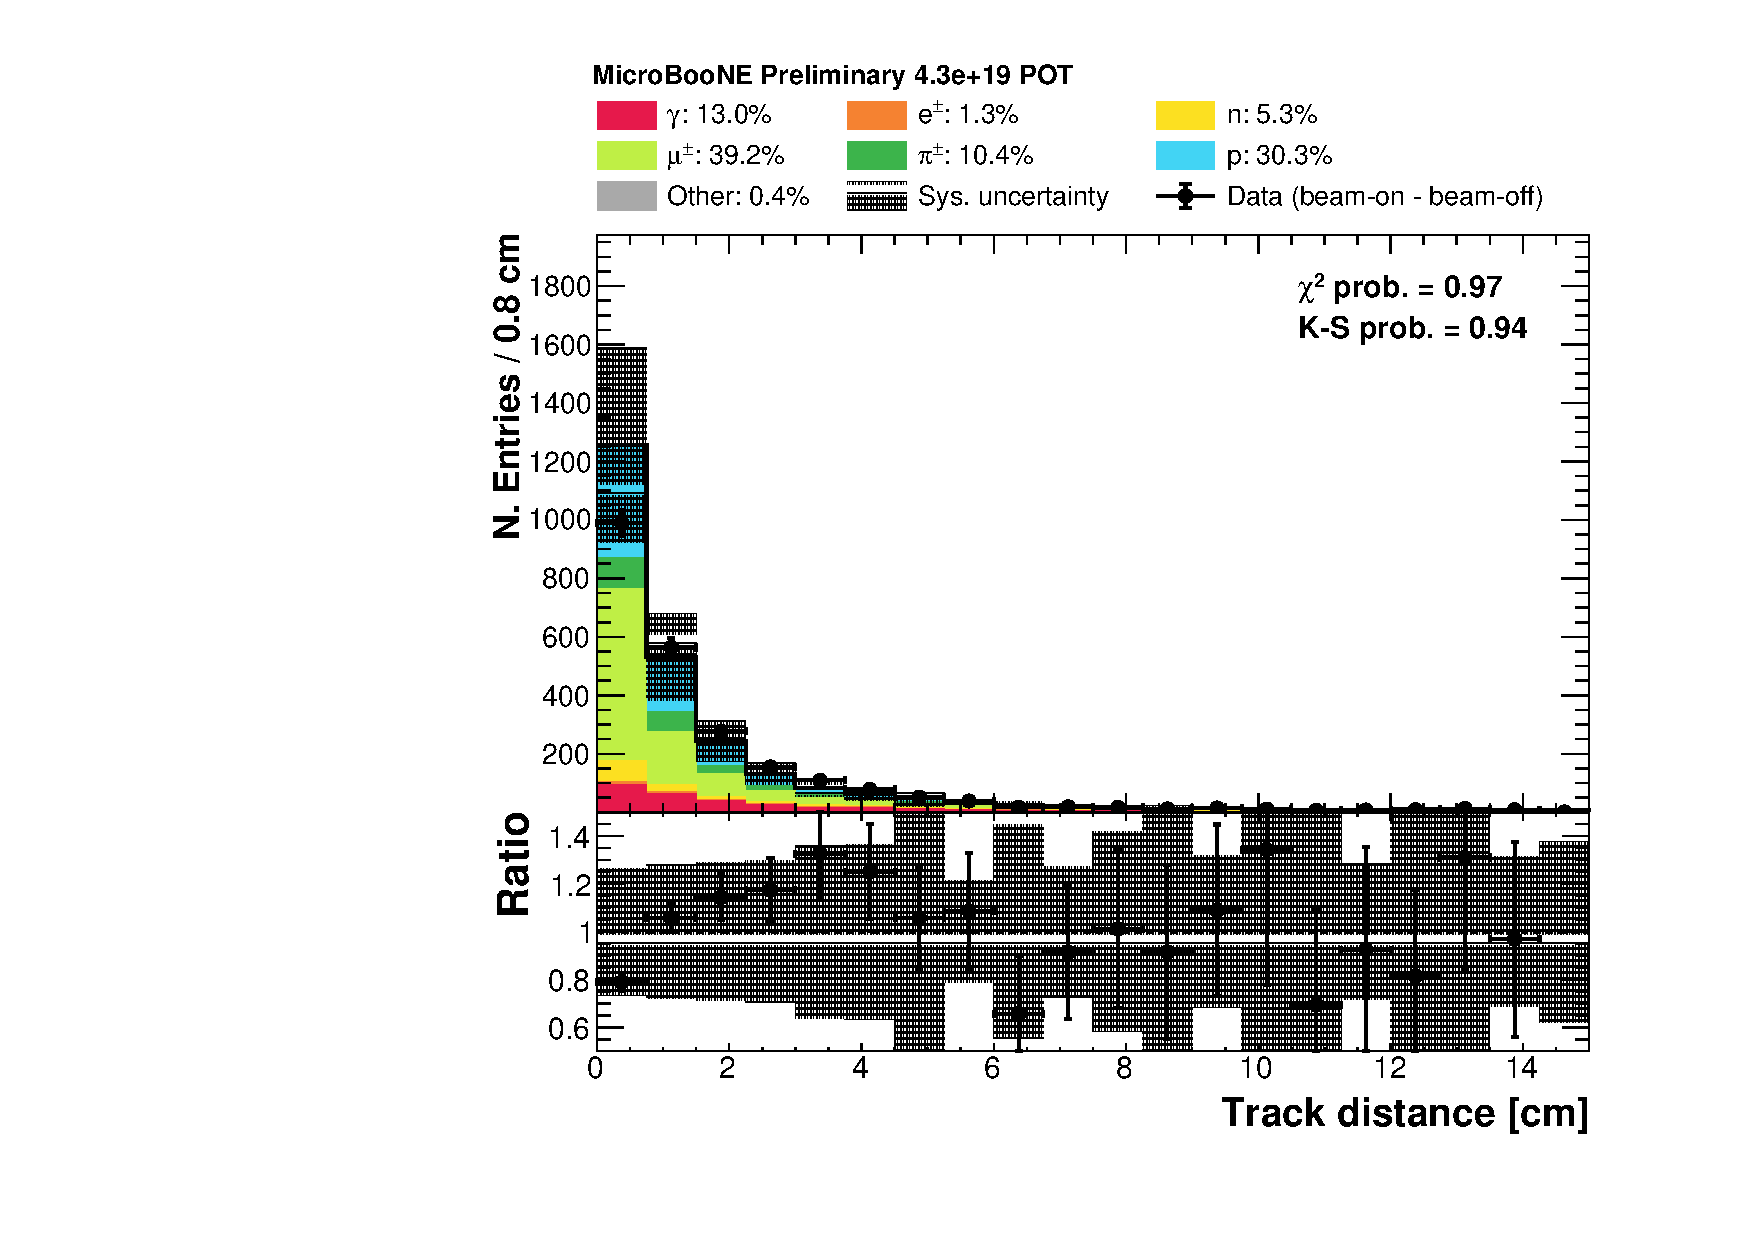
\includegraphics[width=\linewidth]{figures/h_track_distance_pdg.pdf}
    \caption{POT-normalised, generating particle.} \label{fig:trackd_pdg}
  \end{subfigure}
  \begin{subfigure}{0.49\textwidth}
    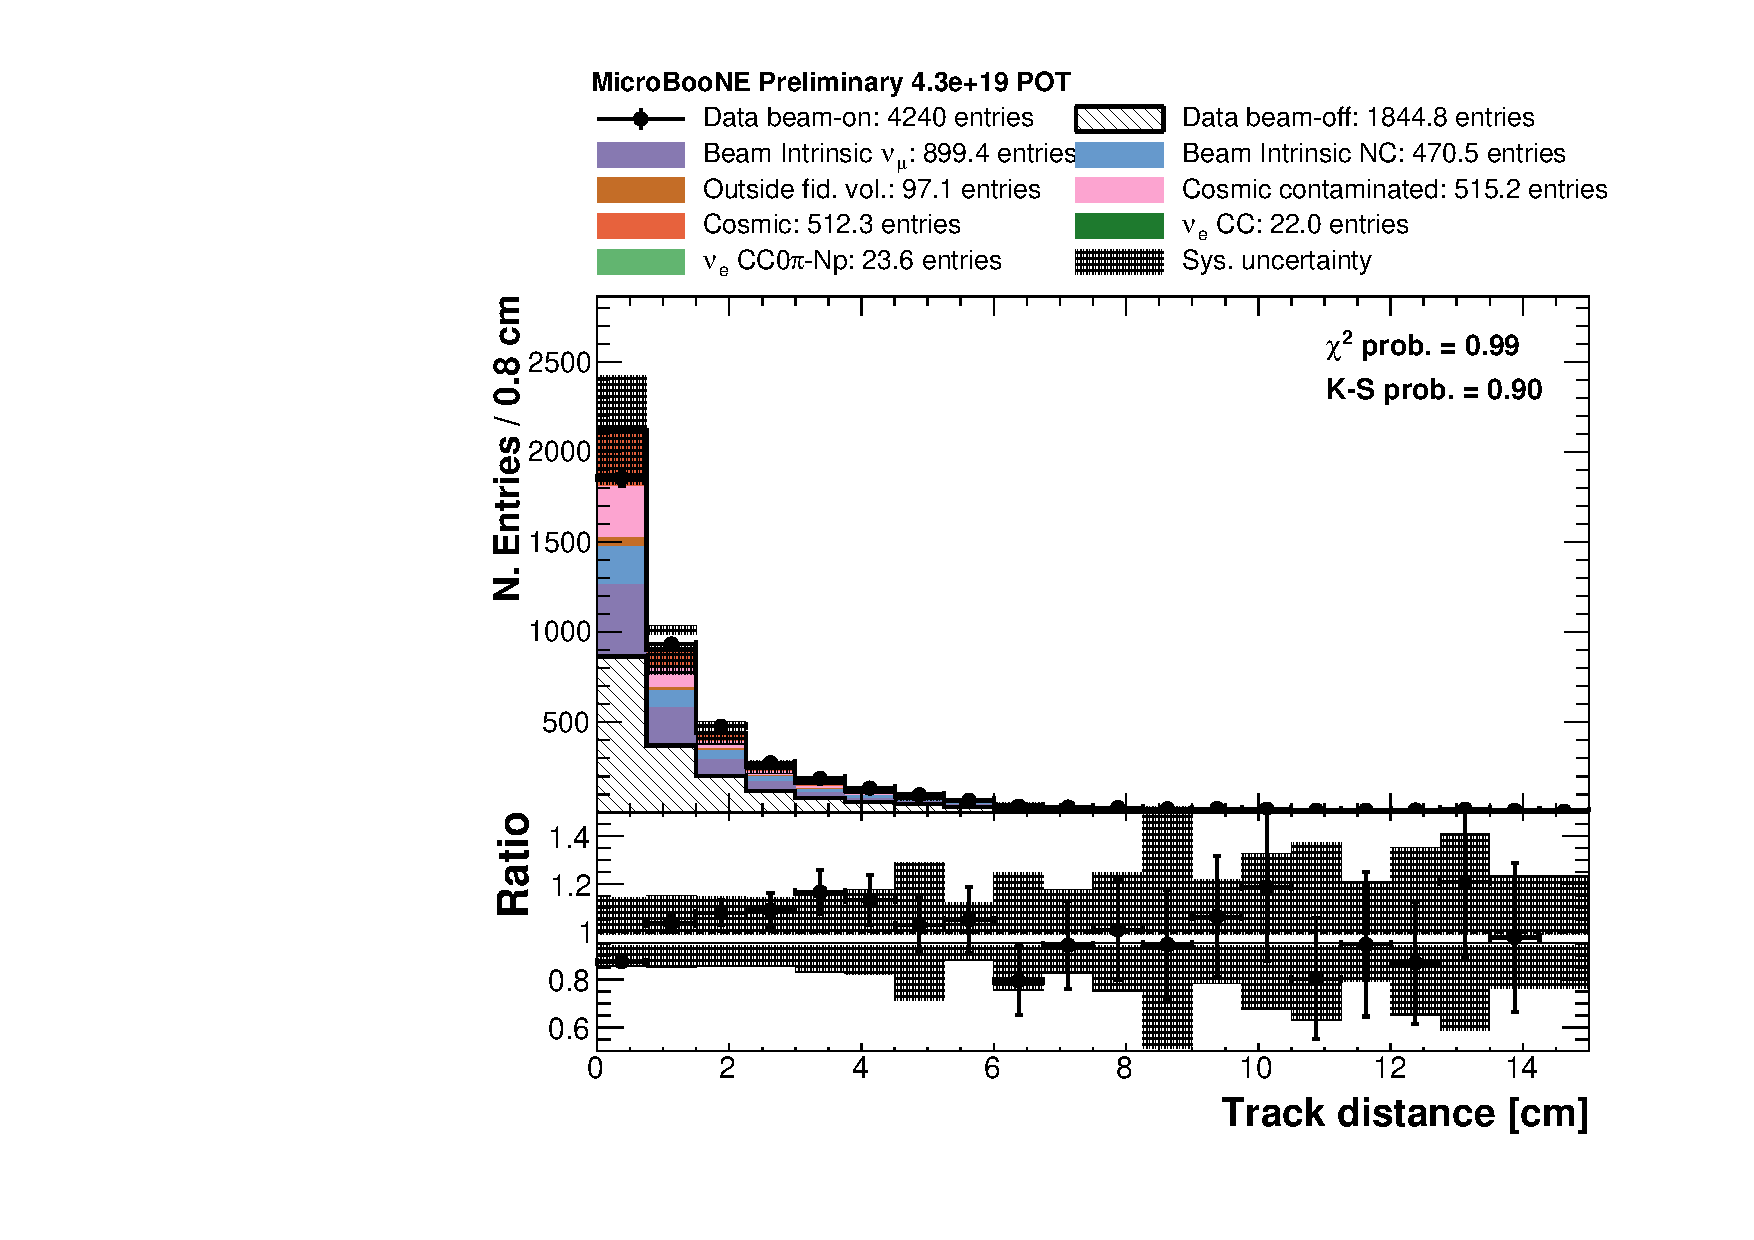
\includegraphics[width=\linewidth]{figures/h_track_distance.pdf}
    \caption{POT-normalised, event category.} \label{fig:trackd_pot}
  \end{subfigure}
  \begin{subfigure}{0.49\textwidth}
    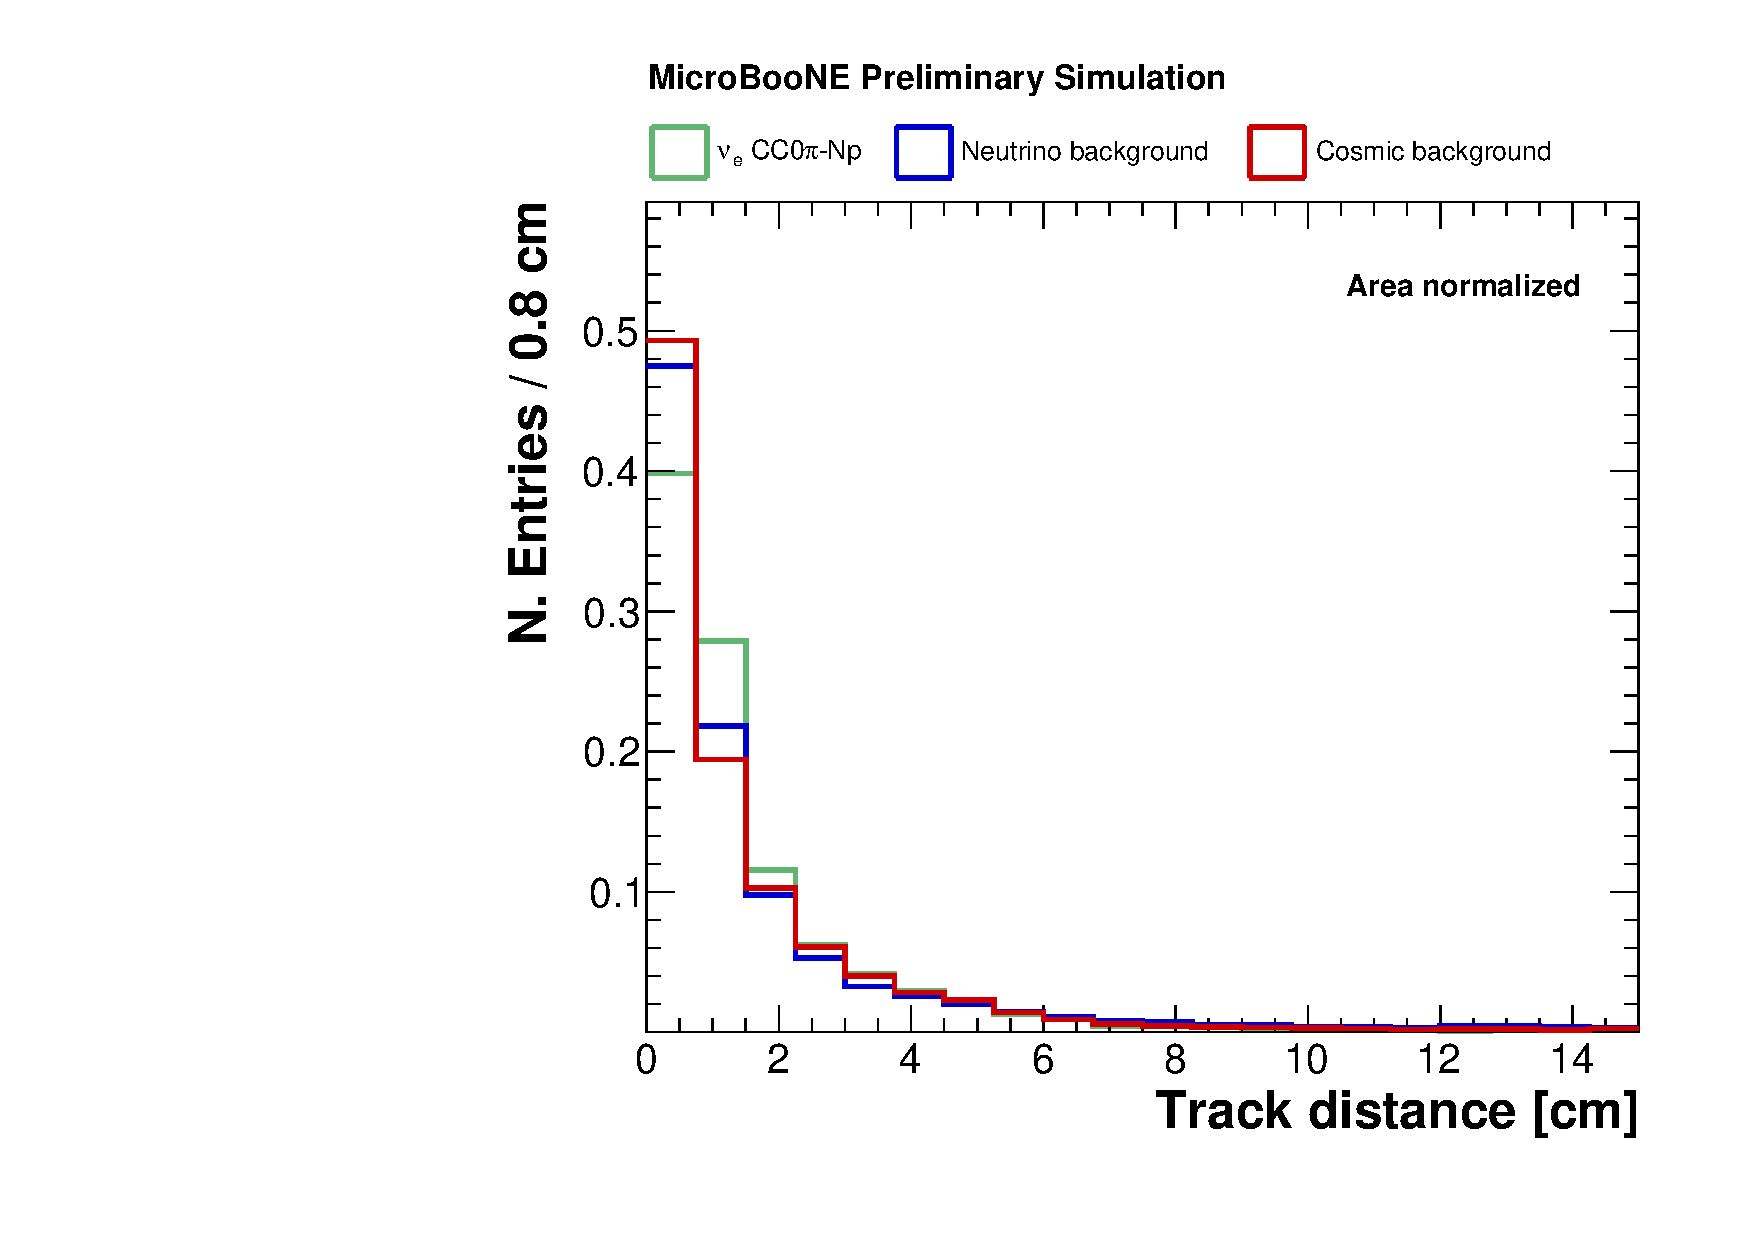
\includegraphics[width=\linewidth]{figures/h_track_distance_norm.pdf}
    \caption{Area-normalised.} \label{fig:trackd_norm}
  \end{subfigure}
  \caption{Area and POT-normalised distributions of the distance between the reconstructed tracks and the reconstructed neutrino vertex.}
\end{figure}

\subsubsection*{Shower distance $d_{s} < 5$~cm}
Liquid argon TPCs such as MicroBooNE can distinguish between photons and electrons in two ways: (1) measuring the $dE/dx$ of the start of the electromagnetic shower, and (2) measuring the gap between the interaction vertex and the start of the electromagnetic shower. Given the interaction length in liquid argon $X_{0}=14$~cm, photons produced in the final state of the neutrino interaction can travel several centimetres without interacting. In order to suppress events with a photon in the final state, the most energetic shower starting point is required to be within 5~cm of the reconstructed neutrino vertex.
Figure \ref{fig:showerd_norm} shows the distributions of the distance between the start point of the reconstructed showers and the reconstructed neutrino vertex for signal and background events. As expected, background neutrino events have a slightly larger tail than the signal events. The agreement between data and Monte Carlo shown in Figure \ref{fig:showerd_pot} {and Figure \ref{fig:showerd_pdg}} is good. Improvements currently implemented in the Pandora framework will allow for more appropriate cuts to further reduce the photon background.

\begin{figure}[htbp]
\centering
  \begin{subfigure}{0.49\textwidth}
    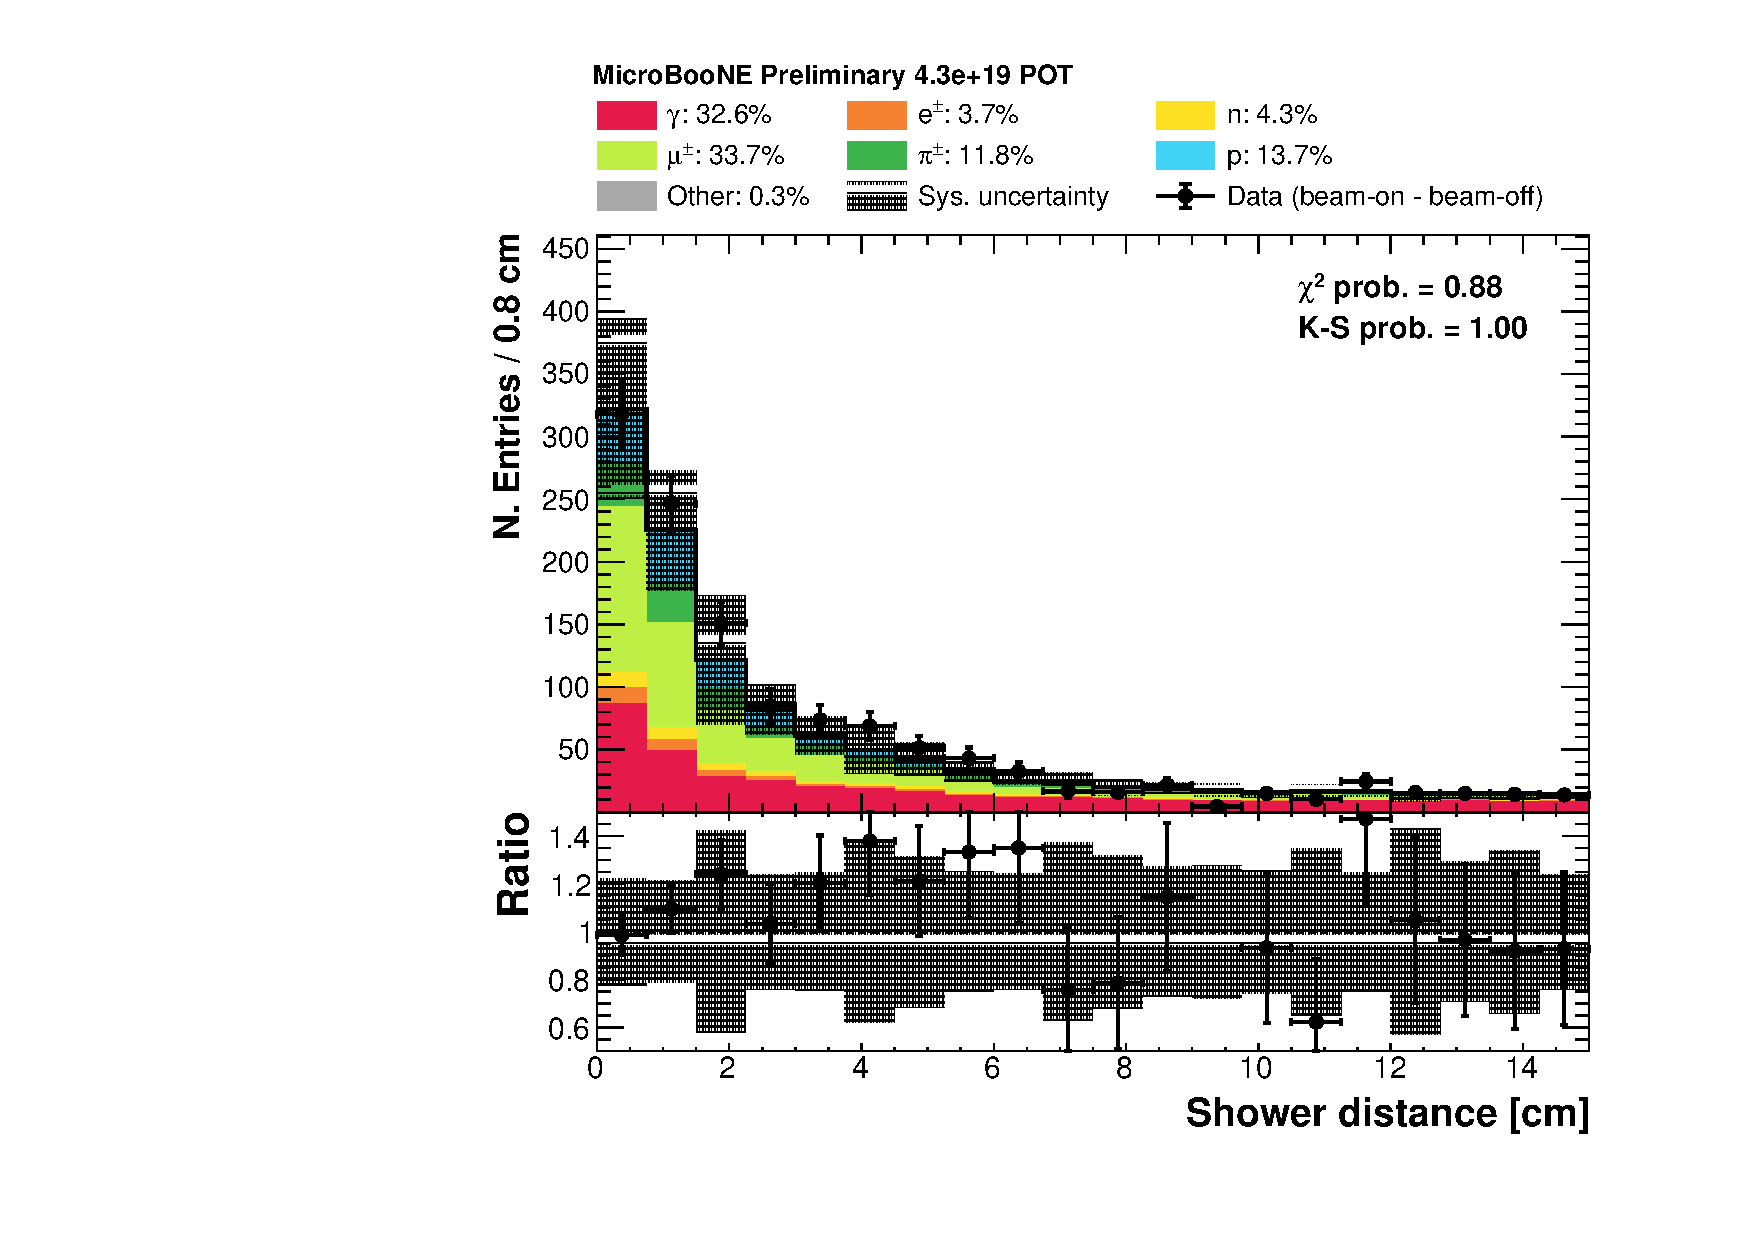
\includegraphics[width=\linewidth]{figures/h_shower_distance_pdg.pdf}
    \caption{POT-normalised, generating particle.} \label{fig:showerd_pdg}
  \end{subfigure}
  \begin{subfigure}{0.49\textwidth}
    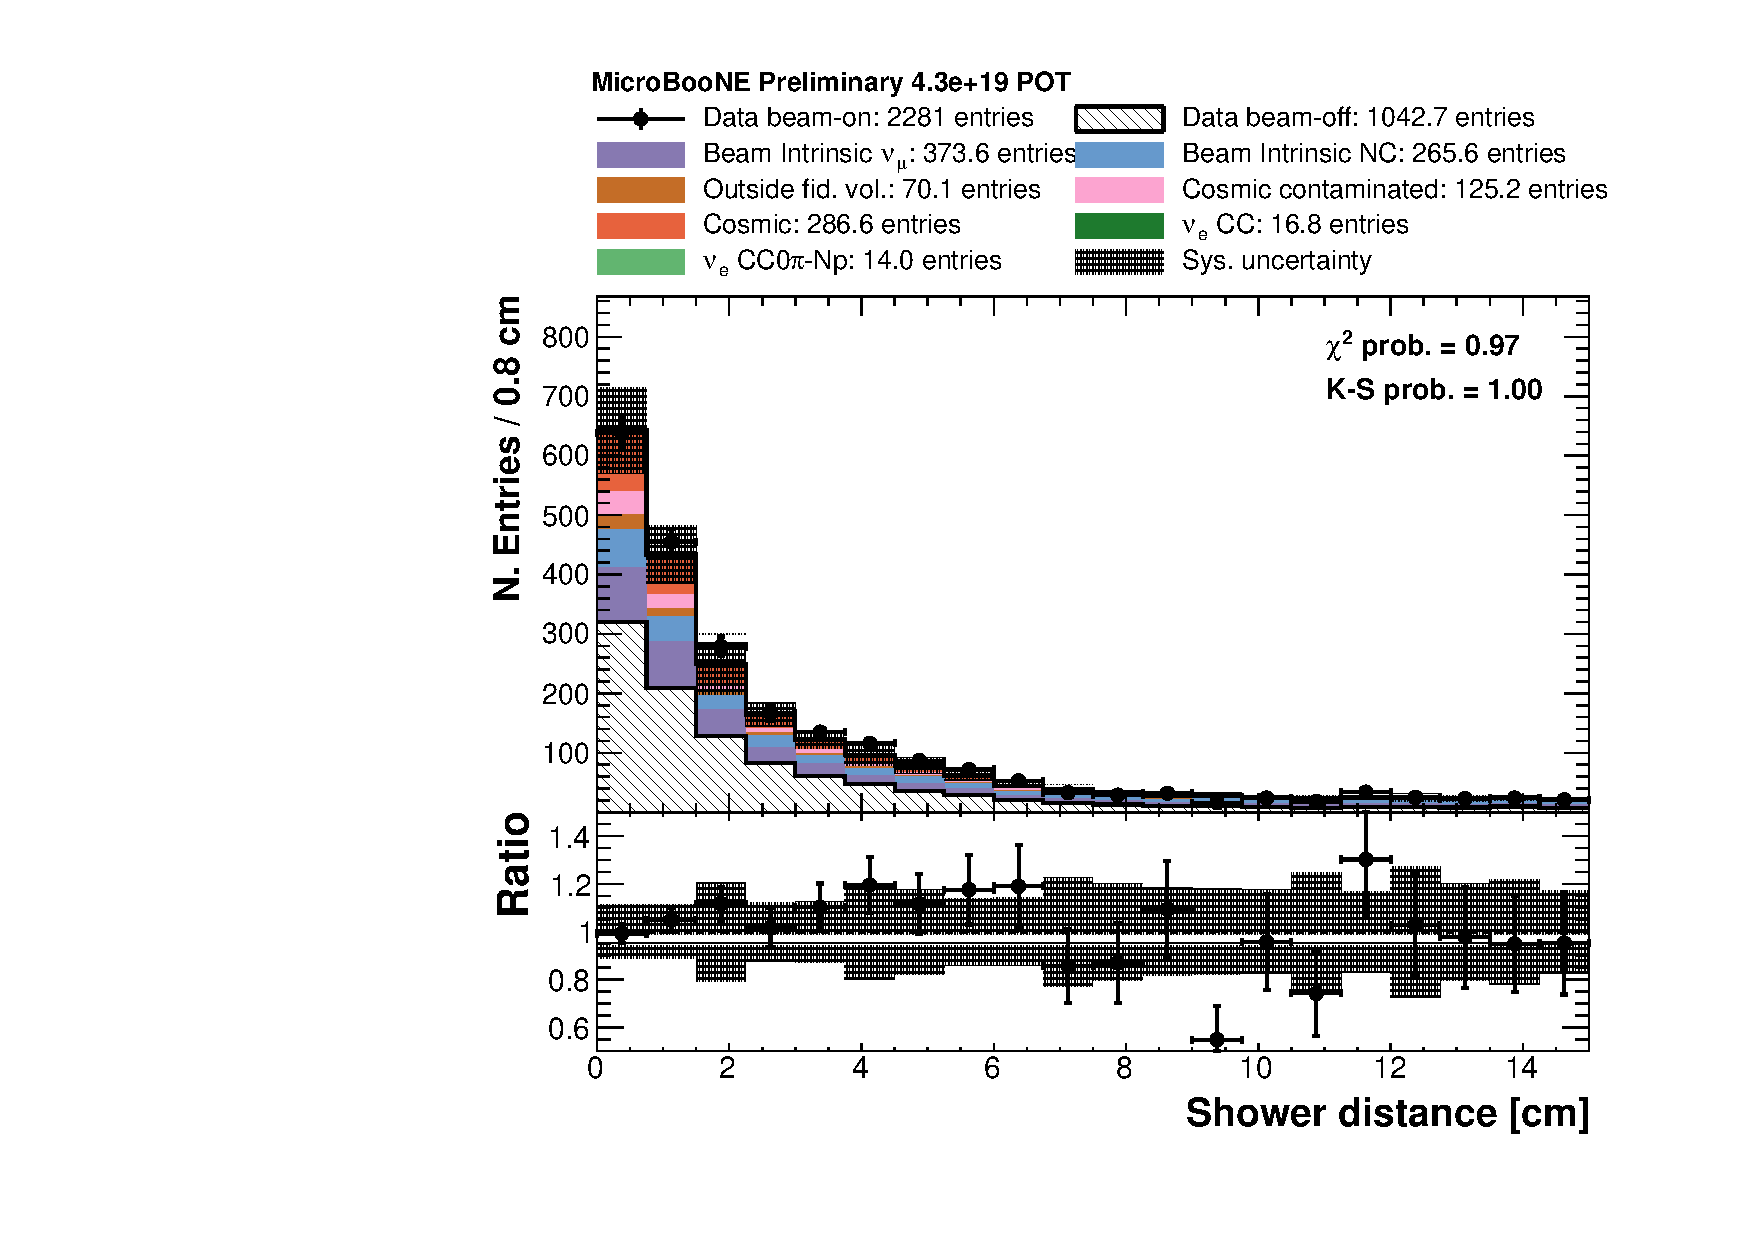
\includegraphics[width=\linewidth]{figures/h_shower_distance.pdf}
    \caption{POT-normalised, event category.} \label{fig:showerd_pot}
  \end{subfigure}
  \begin{subfigure}{0.49\textwidth}
    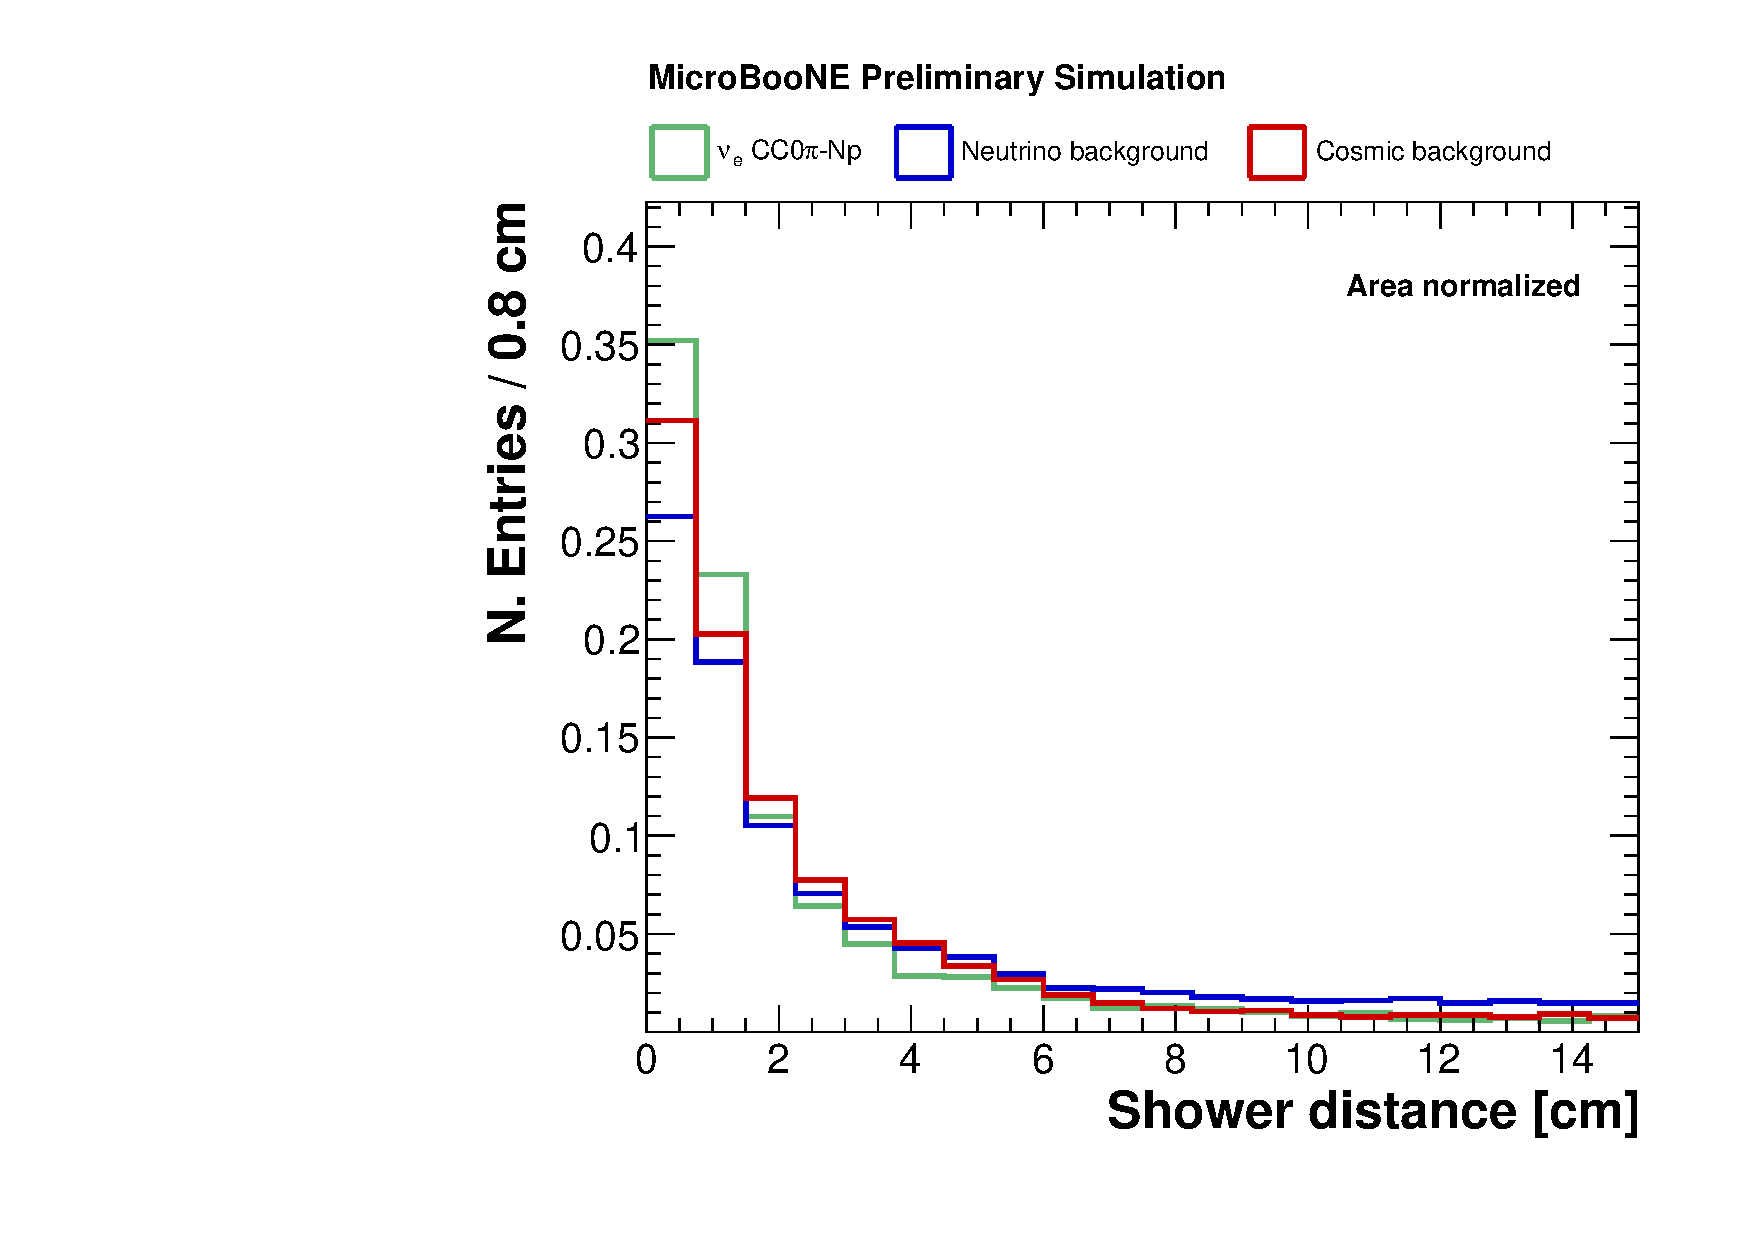
\includegraphics[width=\linewidth]{figures/h_shower_distance_norm.pdf}
    \caption{Area-normalised.} \label{fig:showerd_norm}
  \end{subfigure}
  \caption{Area and POT-normalised distributions of the distance between the reconstructed showers and the reconstructed neutrino vertex.}
\end{figure}

\subsubsection*{Track proton $\chi^2 < 80$}
It is possible to perform a $\chi^2$ test on the $dE/dx$ vs. residual range of the reconstructed track under the hypothesis of a proton stopping in the detector. Low values of the $\chi^2$ score will correspond to proton-like tracks, while a high value will correspond to a MIP-like track. Figure \ref{fig:proton_norm} shows the distributions of the $\chi^2$ score for background and signal events. Figure \ref{fig:proton_pdg} shows that the protons reconstructed as tracks are peaked around 0 as expected, while the long tail includes showers misclassified classified as tracks and events with a misplaced vertex. The comparison between data and Monte Carlo shown in Figure \ref{fig:proton_pot} and Figure \ref{fig:proton_pdg} shows some discrepancies, especially for very low and very high $\chi^2$ scores. This quantity requires a careful simulation of the signal processing and a correct evaluation of the recombination effect. Our cut is in a region with a good data/Monte Carlo agreement once the systematic uncertainties are taken into account and it is as such deemed safe.

\begin{figure}[htbp]
\centering
  \begin{subfigure}{0.49\textwidth}
    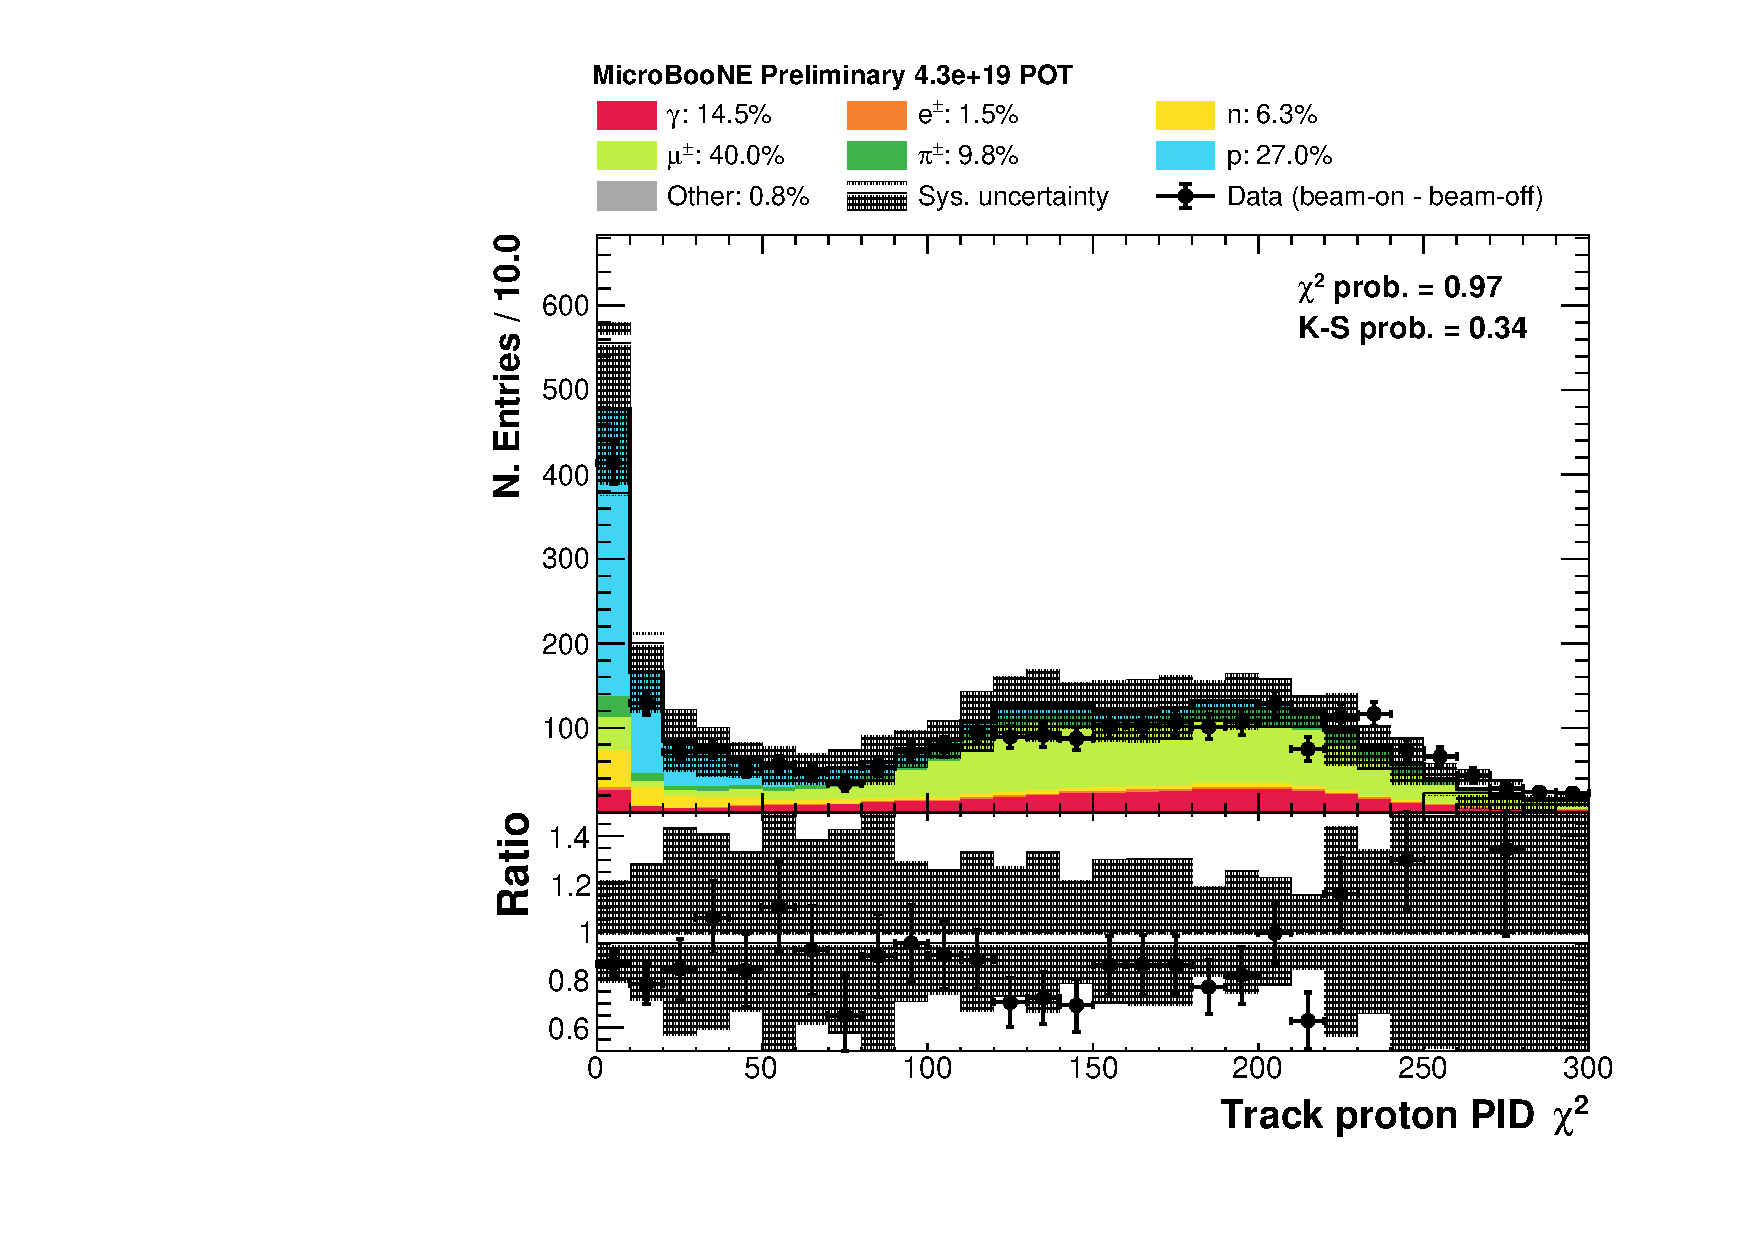
\includegraphics[width=\linewidth]{figures/h_track_pidchipr_pdg.pdf}
    \caption{POT-normalised, generating particle.} \label{fig:proton_pdg}
  \end{subfigure}
  \begin{subfigure}{0.49\textwidth}
    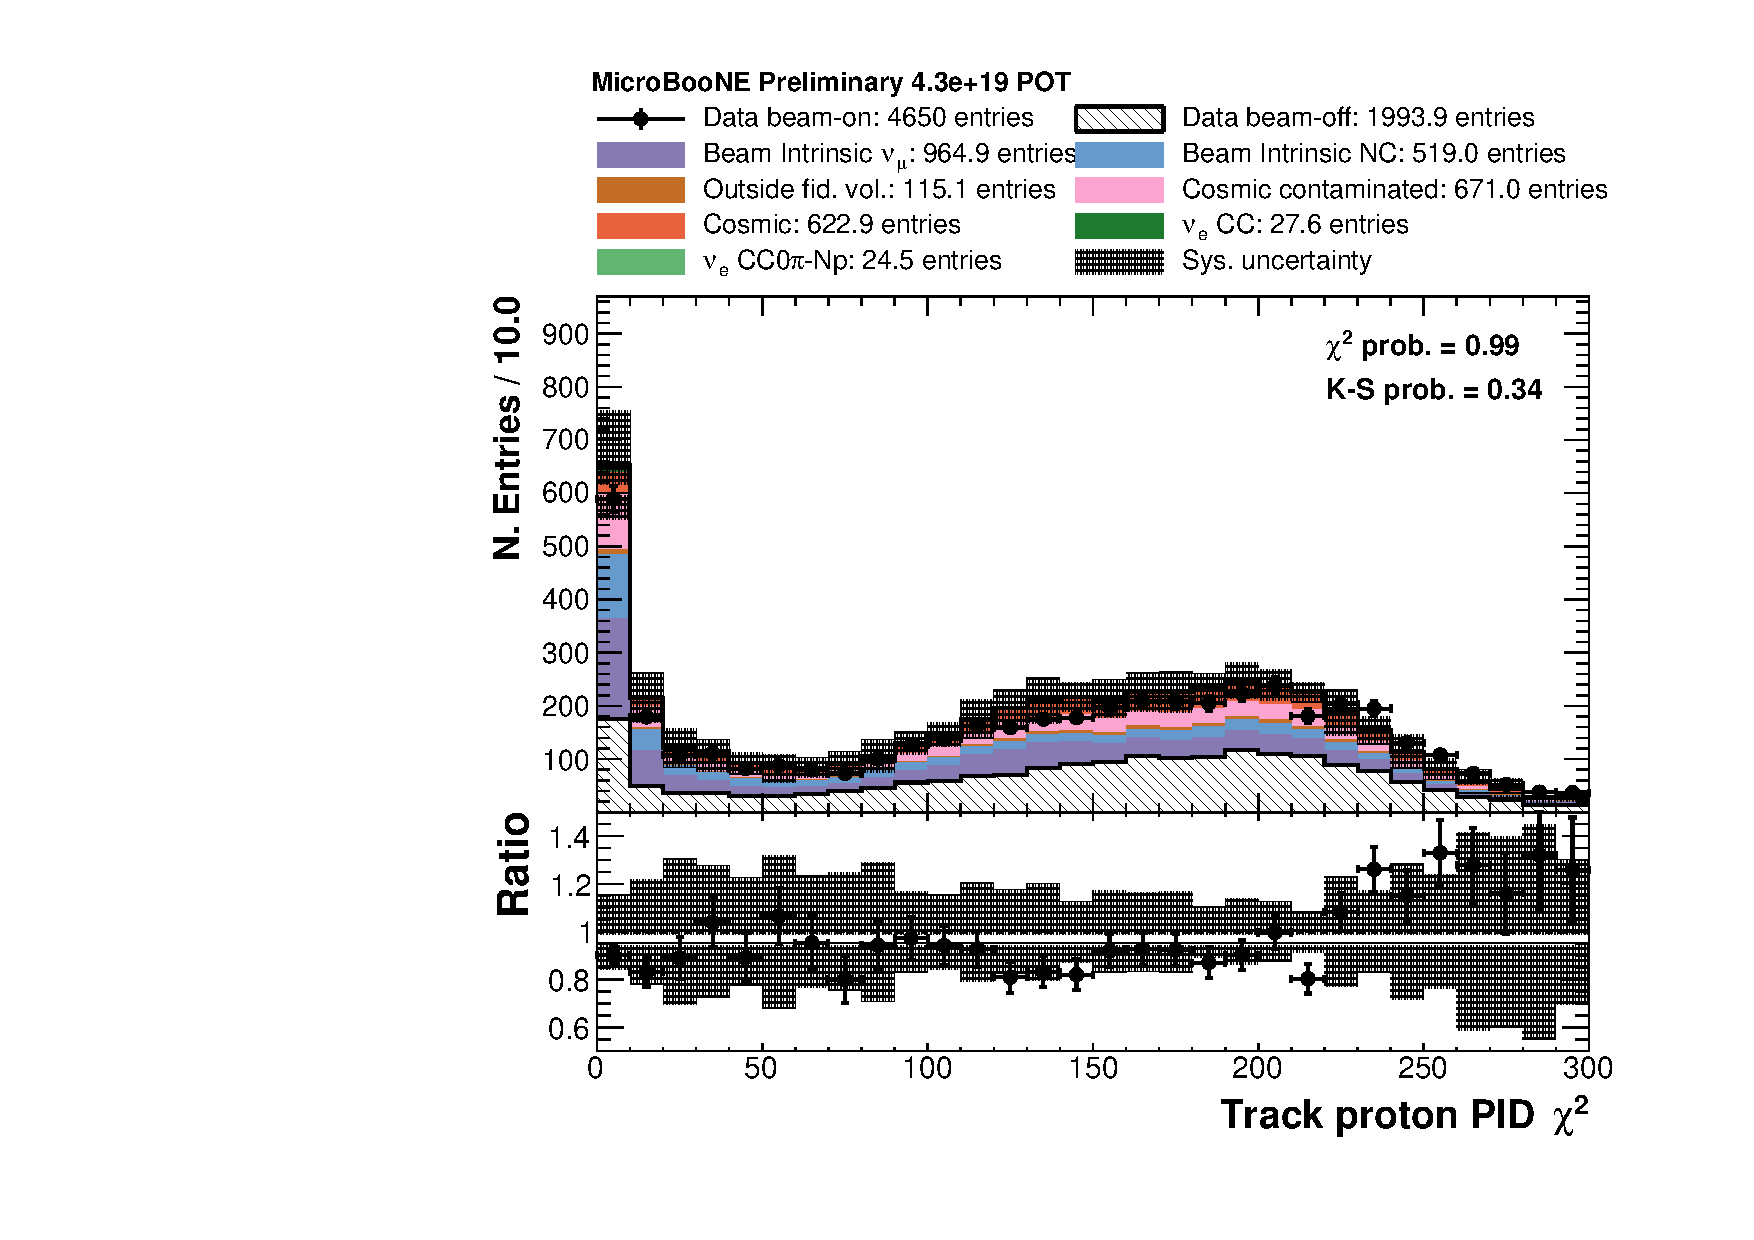
\includegraphics[width=\linewidth]{figures/h_track_pidchipr.pdf}
    \caption{POT-normalised, event category.} \label{fig:proton_pot}
  \end{subfigure}
  \begin{subfigure}{0.49\textwidth}
    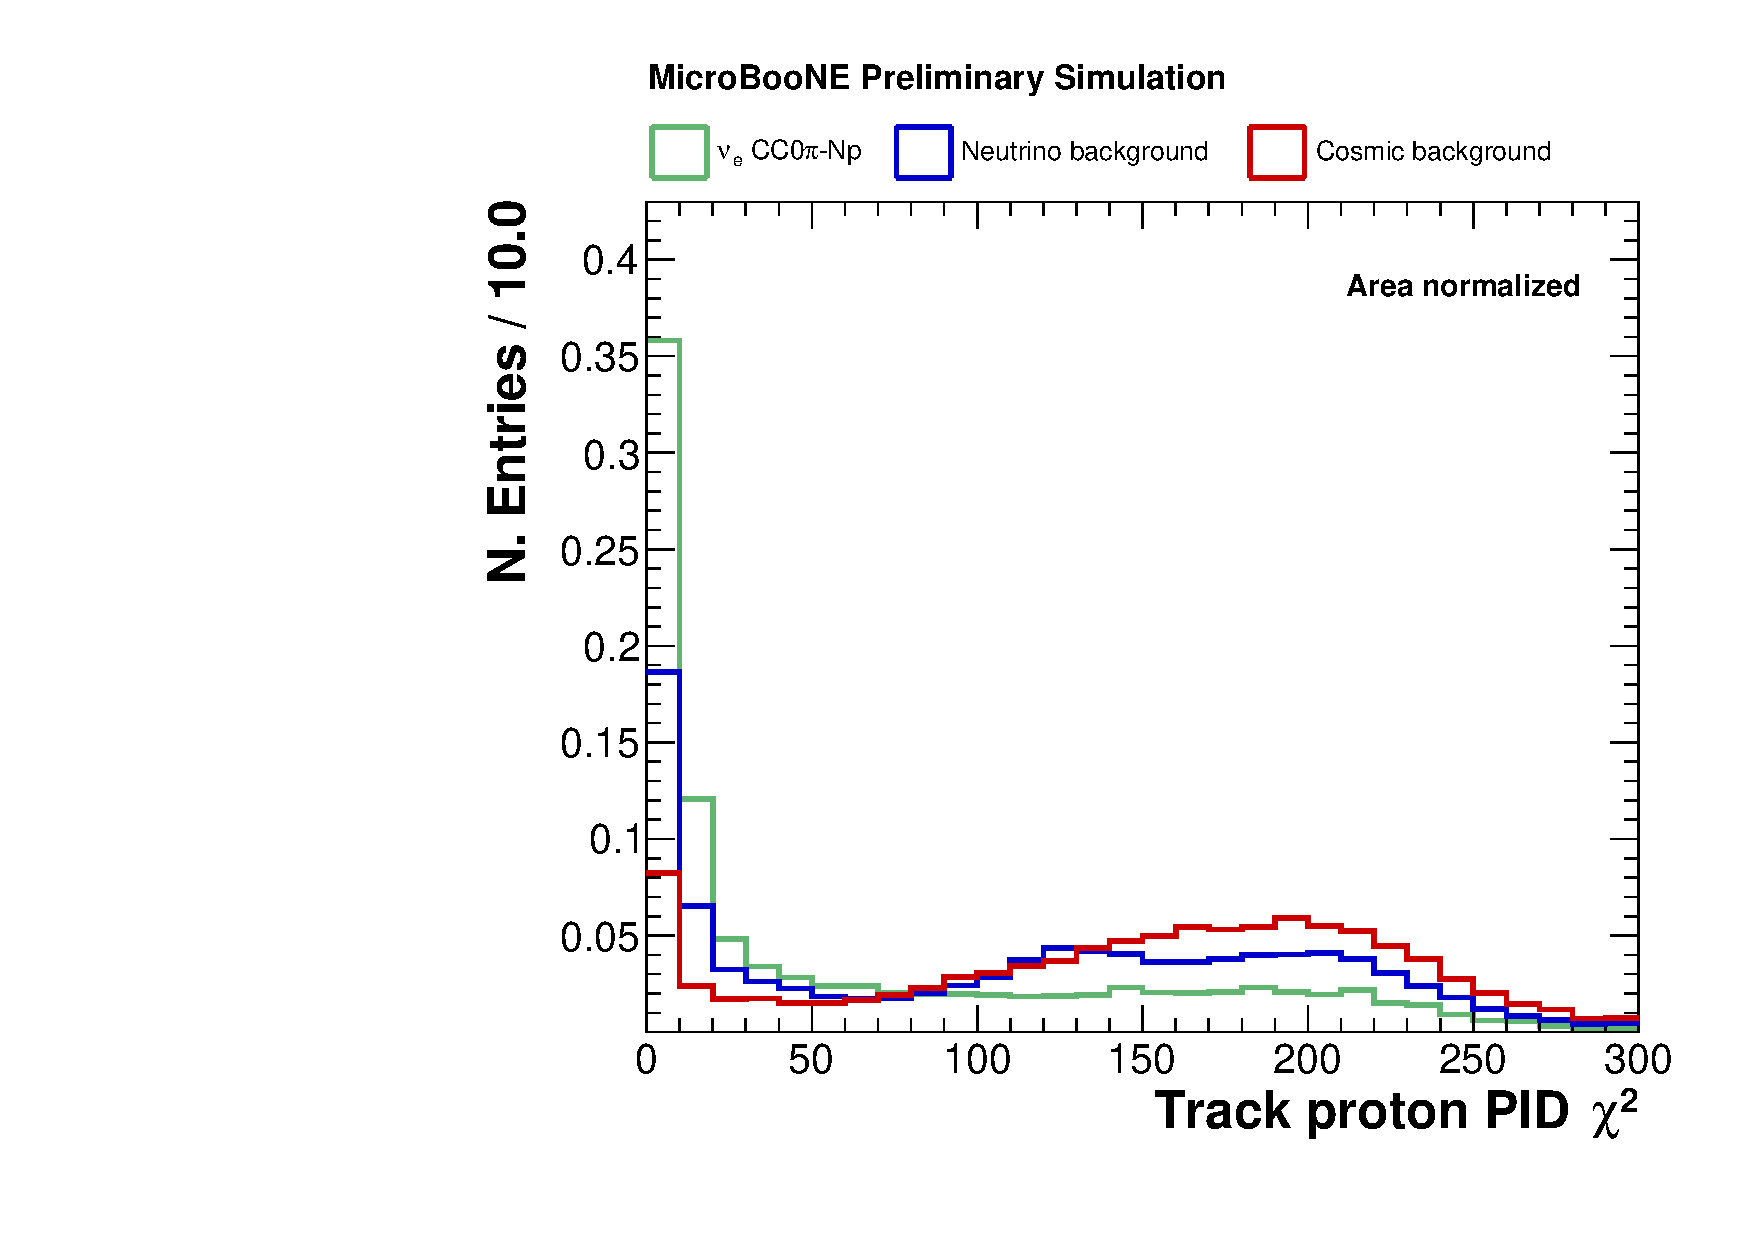
\includegraphics[width=\linewidth]{figures/h_track_pidchipr_norm.pdf}
    \caption{Area-normalised.} \label{fig:proton_norm}
  \end{subfigure}
  \caption{Area and POT-normalised distributions of the proton $\chi^2$ score of the reconstructed tracks, classified according to the event category and to the primary particle generating the shower.}\label{fig:proton_bkg}
\end{figure}

\subsubsection*{Track-shower angle $\mathrm{cos}\alpha > -0.95$}
Electrons start producing an appreciable shower in the detector after several centimetres. In this case, the reconstruction framework often identifies the first part of the shower as a track-like object and the latter part of the shower as a shower-like object. 
Furthermore, high-energy cosmic rays can produce a shower in the detector, which will be mostly aligned to a cosmic muon track. In order to remove these mis-reconstructed events and reduce this kind of cosmogenic background we require $\mathrm{cos}\alpha > -0.95$, where $\alpha$ is the angle between the most energetic shower and the track with the lowest proton $\chi^2$ score.
Figure \ref{fig:angle_integral} shows that there are, in proportion, more background events with a high angular separation between the most proton-like track and the most energetic shower. This cut allows to reject these events while also ensuring that the signal events are well-reconstructed. In fact, signal events with $\mathrm{cos}\alpha \approx -1$ have almost always an electron shower reconstructed as a track-like object in the first part. The agreement shown in Figure \ref{fig:angle_pot} and Figure \ref{fig:angle_pdg} is good. Future improvements to the shower reconstruction will allow for an increased selection efficiency.

\begin{figure}[htbp]
\centering
  \begin{subfigure}{0.49\textwidth}
    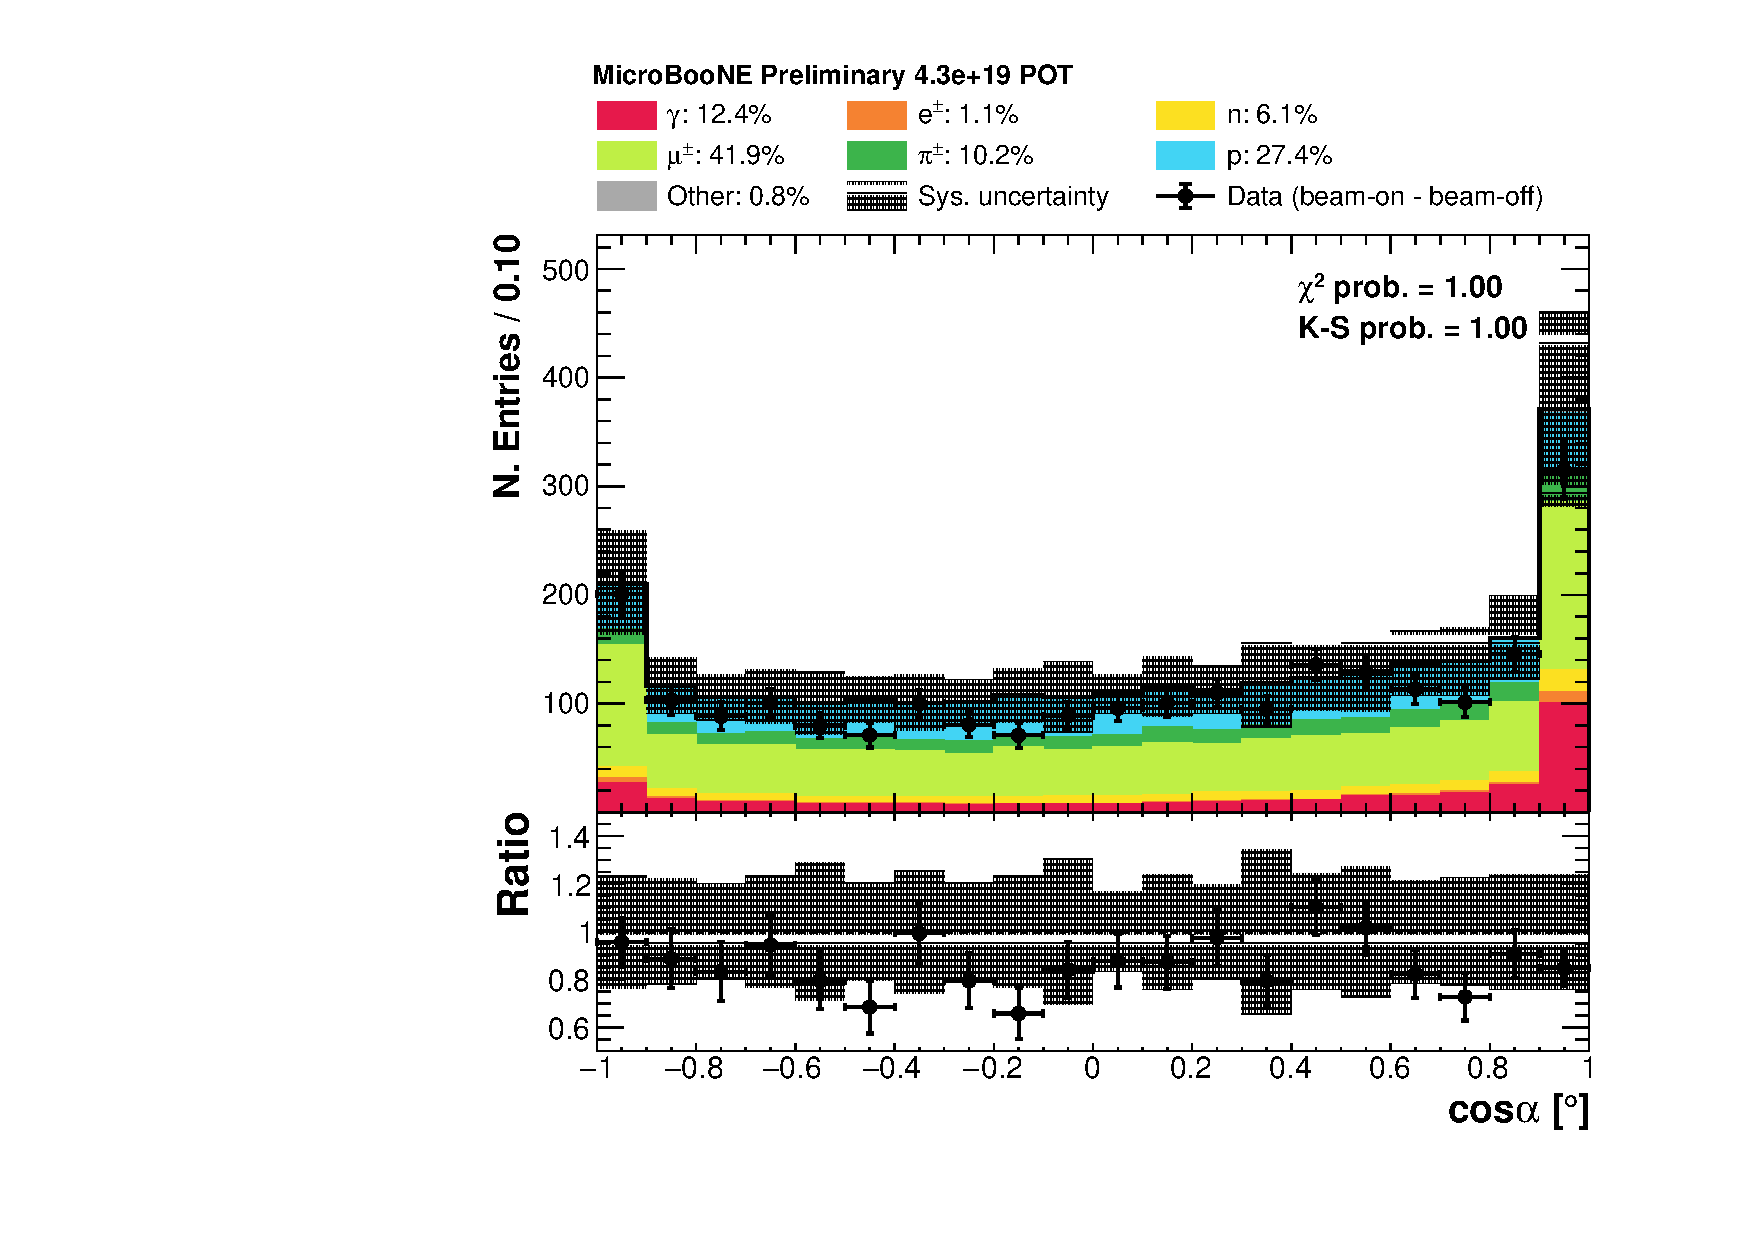
\includegraphics[width=\linewidth]{figures/h_track_shower_angle_pdg.pdf}
    \caption{POT-normalised, generating particle.} \label{fig:angle_pdg}
  \end{subfigure}
  \begin{subfigure}{0.49\textwidth}
    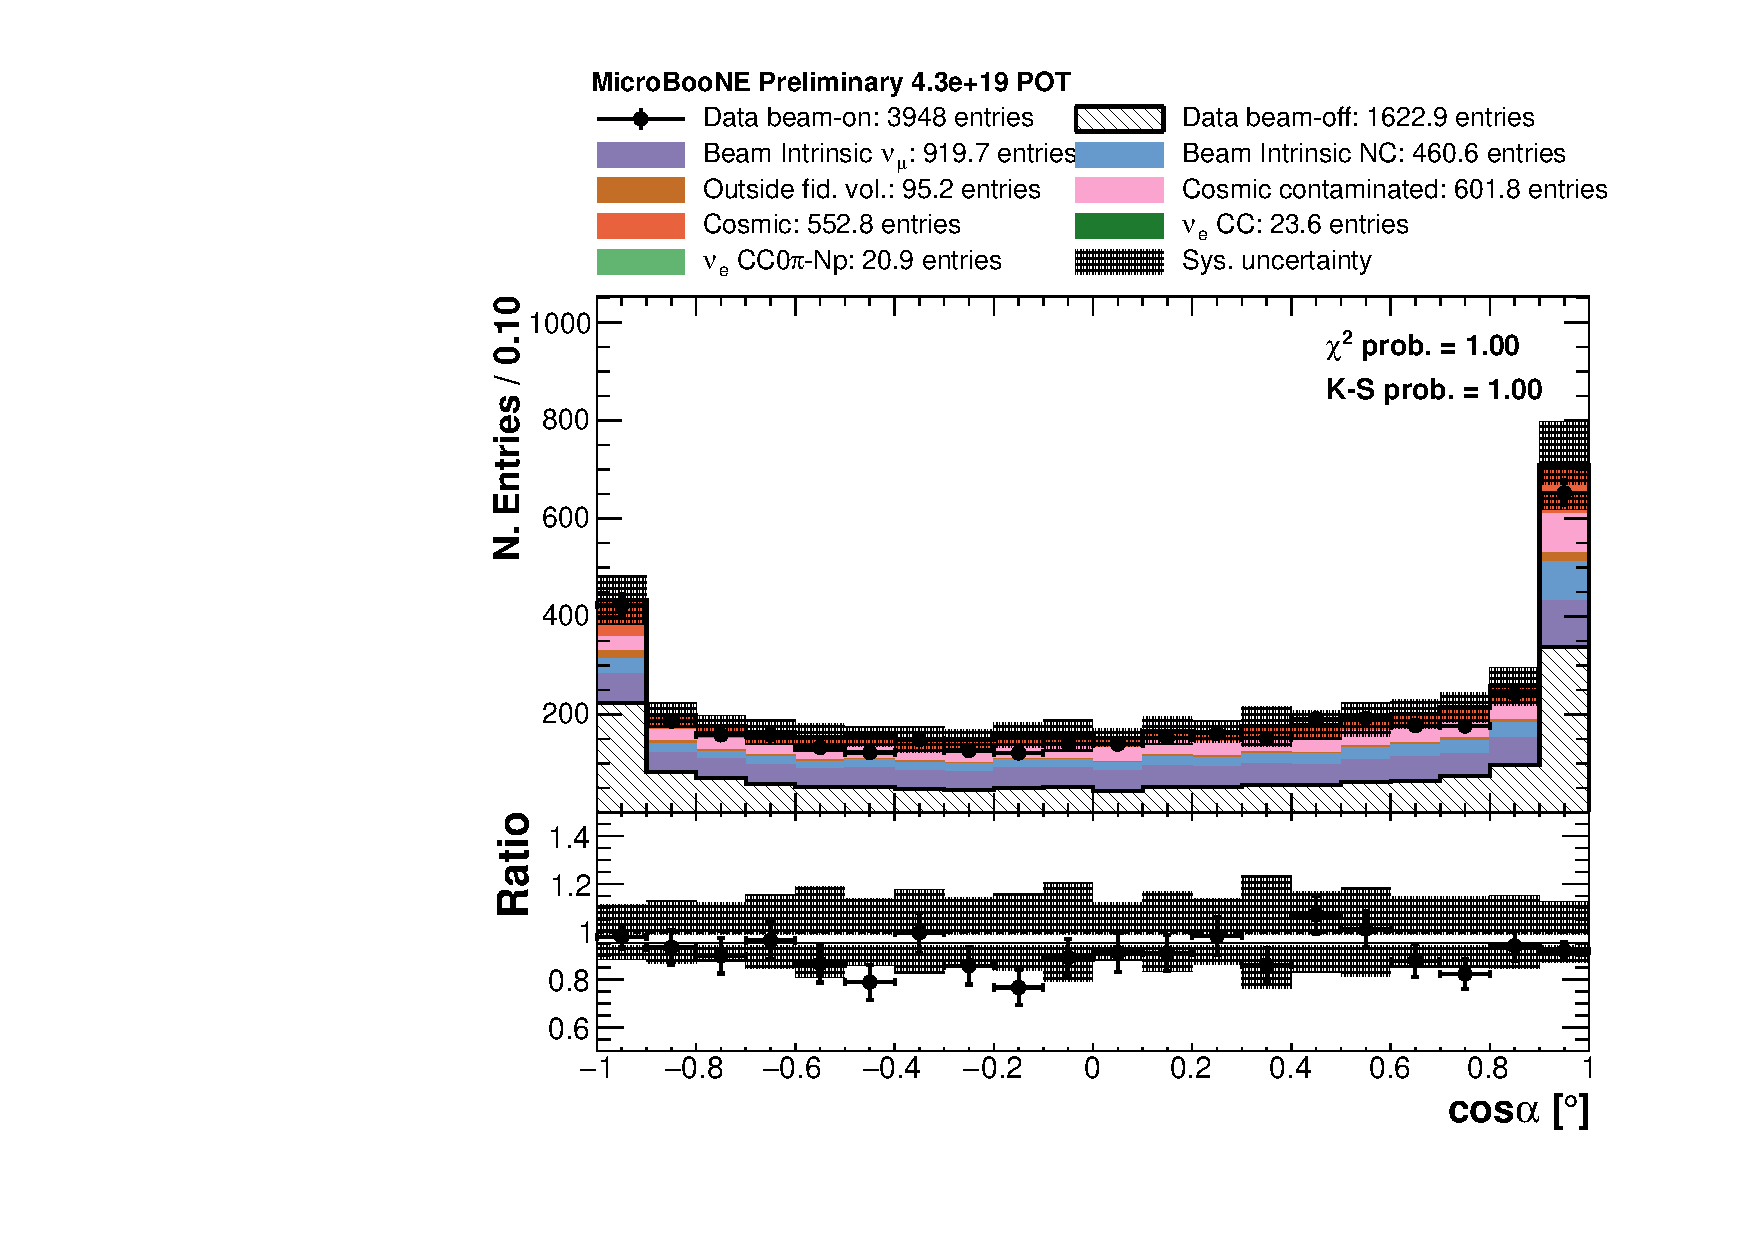
\includegraphics[width=\linewidth]{figures/h_track_shower_angle.pdf}
    \caption{POT-normalised, event category.} \label{fig:angle_pot}
  \end{subfigure}

    \begin{subfigure}{0.49\textwidth}
    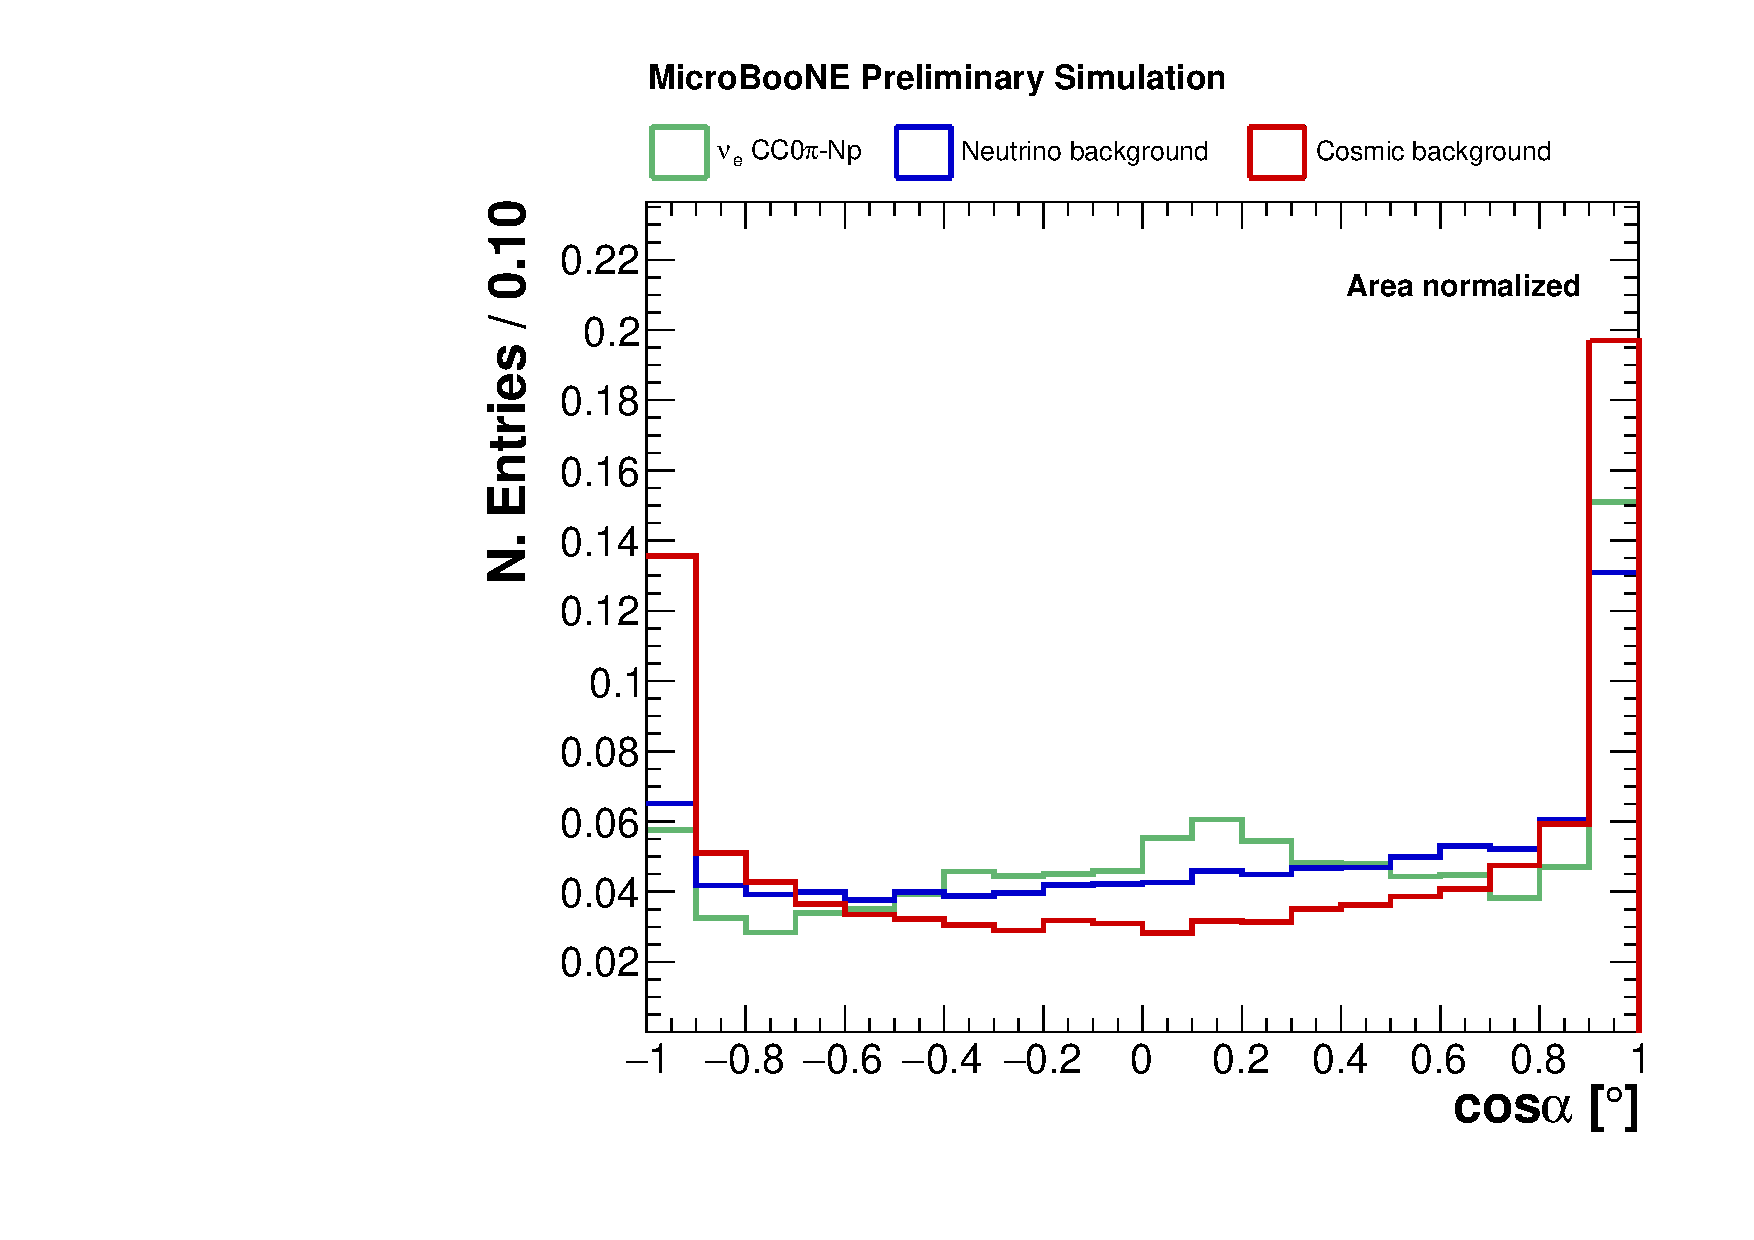
\includegraphics[width=\linewidth]{figures/h_track_shower_angle_norm.pdf}
    \caption{Area-normalised.} \label{fig:angle_integral}
  \end{subfigure}
  \caption{Area and POT-normalised distributions of the angle $\alpha$ between each reconstructed track and the leading shower, classified according to the event category and to the primary particle generating the shower.}
\end{figure}

\subsubsection*{Most proton-like track length $L < 80~\mathrm{cm}$}
Our signal sample will contain only protons in the final state. Protons in liquid argon have a higher stopping power than muons, which will correspond on average to shorter tracks. The track with the lowest $\chi^{2}$ proton score is required to be shorter than 80 cm. This cut helps rejecting mainly CC $\nu_{\mu}$ events with high-energy muons in the final state. 
Both neutrino and cosmic background events have on average longer reconstructed tracks than signal events, as shown in Figure \ref{fig:length_norm}. The cut $L < 80~$cm increases the signal purity without significantly decreasing the signal efficiency. The agreement between data and Monte Carlo distributions is good (Figures \ref{fig:length_pot}, \ref{fig:length_pdg}). A dedicated particle identification algorithm currently under development will replace this cut in the future.

\begin{figure}[htbp]
\centering
  \begin{subfigure}{0.49\textwidth}
    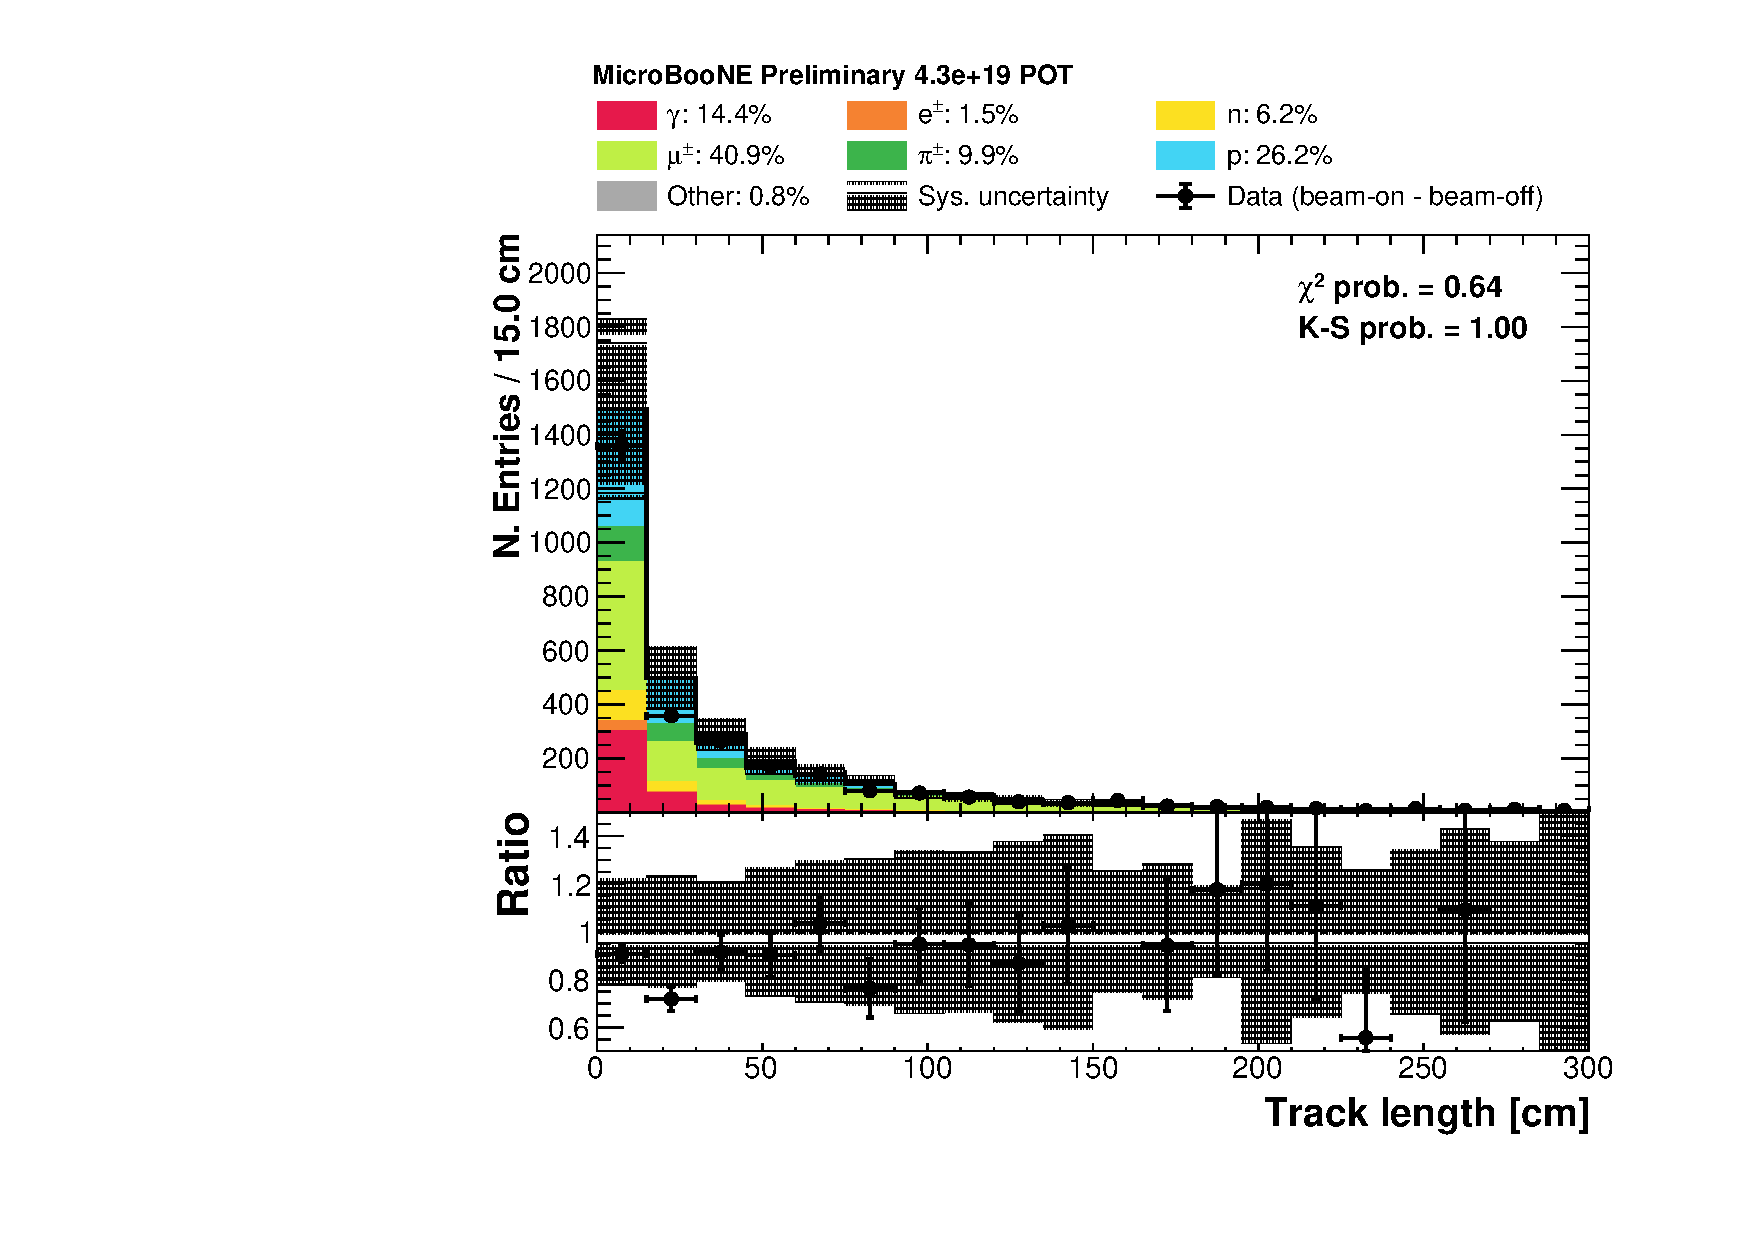
\includegraphics[width=\linewidth]{figures/h_track_length_pdg.pdf}
    \caption{POT-normalised, generating particle.} \label{fig:length_pdg}
  \end{subfigure}
  \begin{subfigure}{0.49\textwidth}
    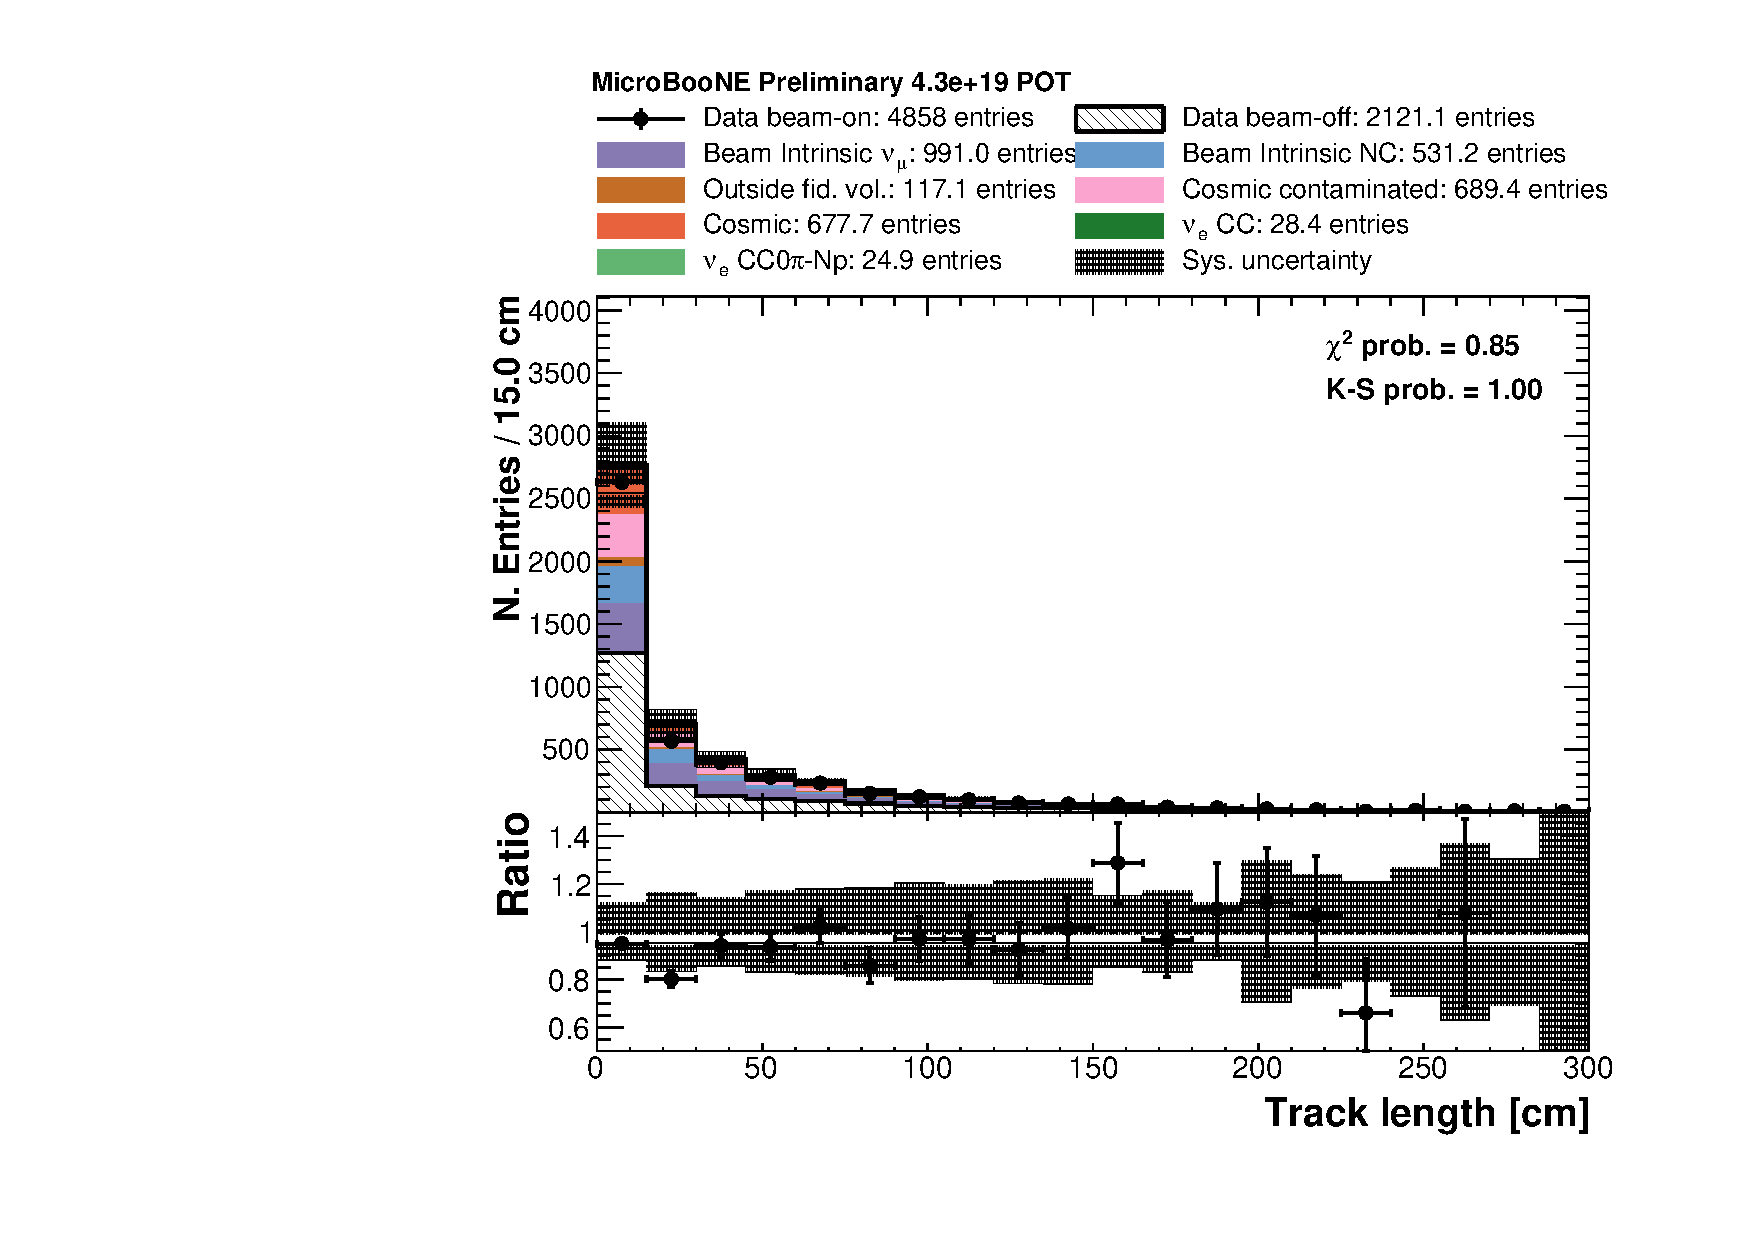
\includegraphics[width=\linewidth]{figures/h_track_length.pdf}
    \caption{POT-normalised, event category.} \label{fig:length_pot}
  \end{subfigure}
    \begin{subfigure}{0.49\textwidth}
    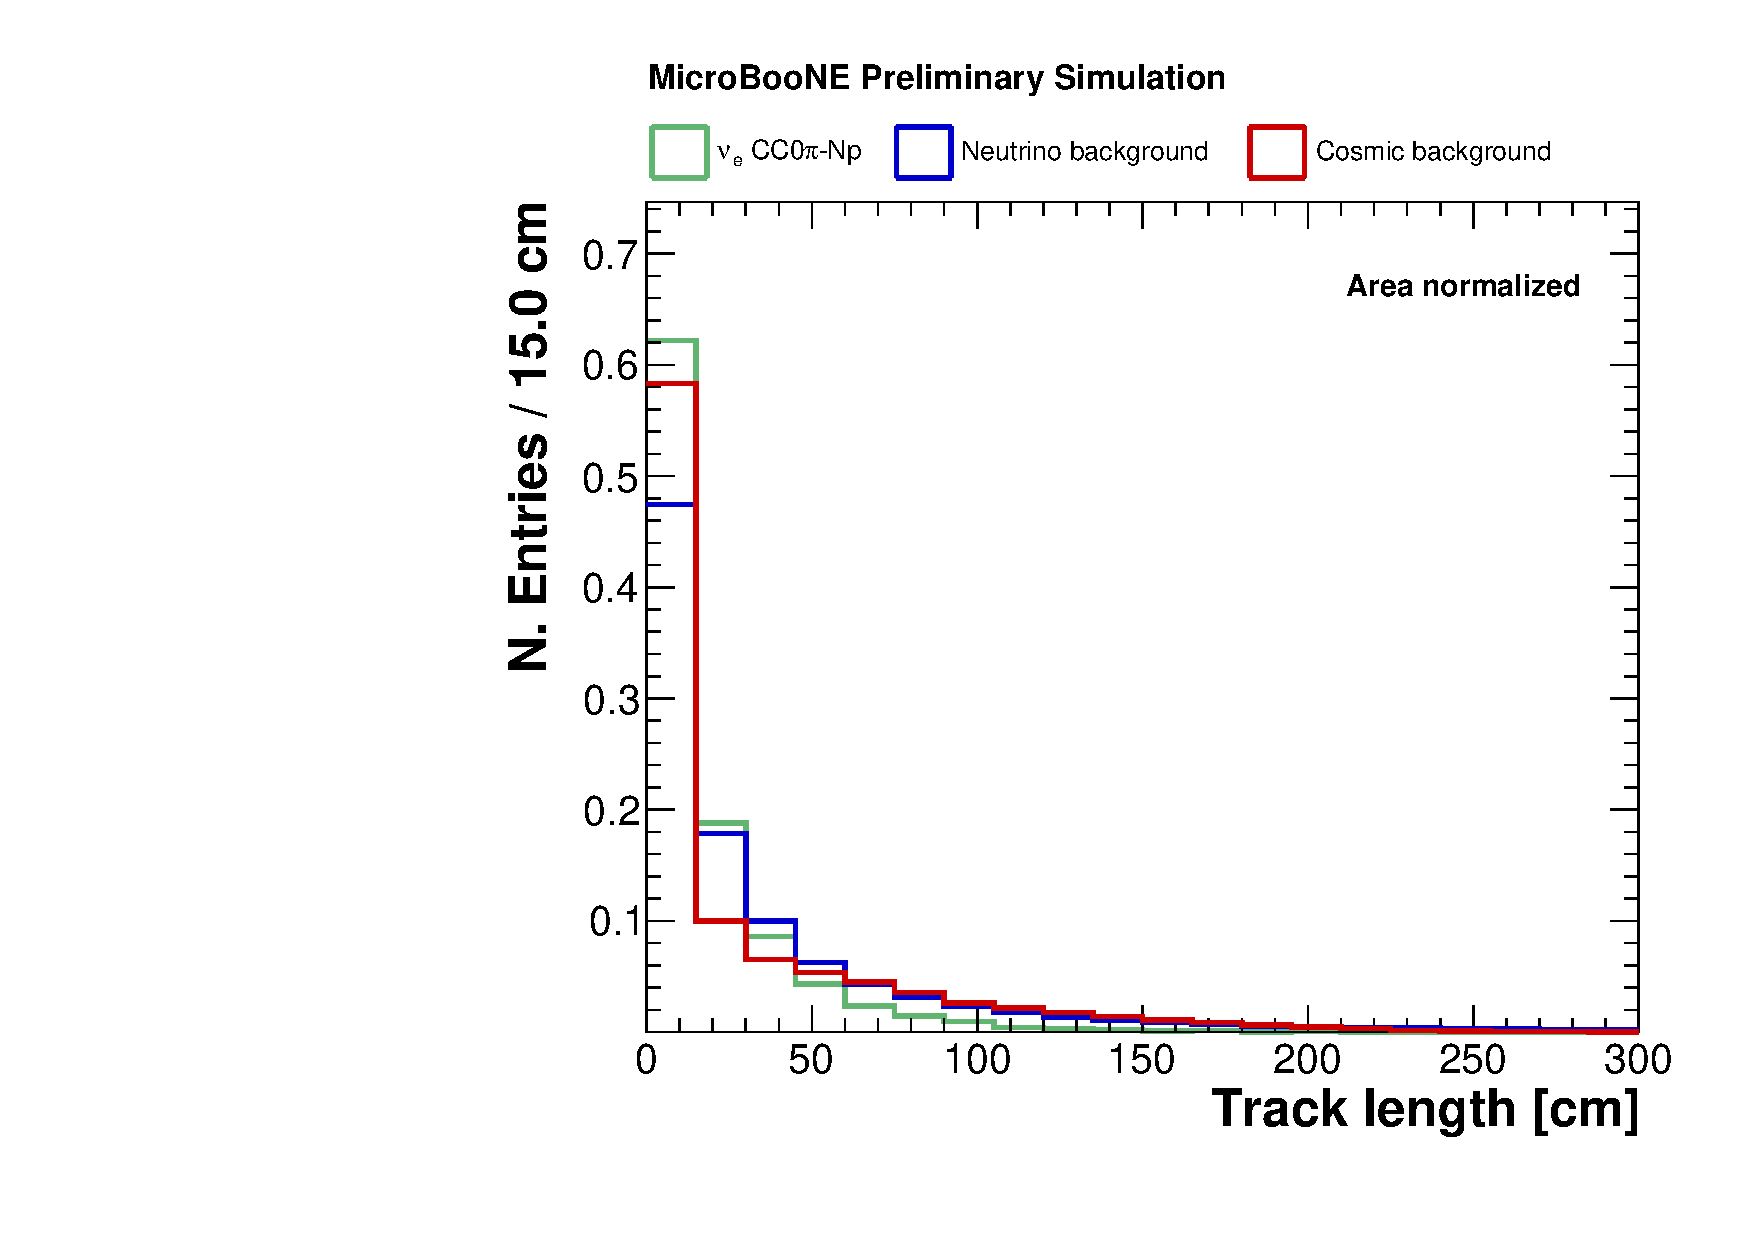
\includegraphics[width=\linewidth]{figures/h_track_length_norm.pdf}
    \caption{Area-normalised.} \label{fig:length_norm}
  \end{subfigure}
  \caption{Area and POT-normalised distributions of the reconstructed tracks, classified according to the event category and to the primary particle generating the shower.}
\end{figure}

\subsubsection*{Rectangular cuts selection results}
The goal of the rectangular cuts is to isolate the $\nu_e$ CC0$\pi$-Np events and increase the purity of our selected sample. However, in order to validate our cuts and verify the agreement between data and Monte Carlo also after this stage, it is necessary to select also a sufficient number of data events. In particular, in this analysis we require at least one data event in the bins in the $[0.2,1.9]$~GeV range, which is also the energy region we are most interested into. 


We select 16 data beam-on events, 2.8 beam-off events, and 12.4 simulated events. The number of selected $\nu_e$ CC0$\pi$-Np events is $3.2$, which corresponds to a final efficiency of $(10.0\pm0.3~\mathrm{(stat)}\pm0.5~\text{(sys)})\%$. 

The purity of the sample is defined as:
\begin{equation}
P = \frac{\mathrm{N.~of~selected~\nu_e~CC0}\pi\mathrm{{\text -}Np~events}}{\mathrm{N.~of~selected~events}}
\end{equation}
Figure \ref{fig:purity_sel} shows the purity before and after the application of the rectangular cuts as a function of the reconstructed energy $E_{\mathrm{deposited}}$. It increase by a factor of 40, from 0.5\% to 21.2\%.

\begin{figure}[htbp]
\centering
  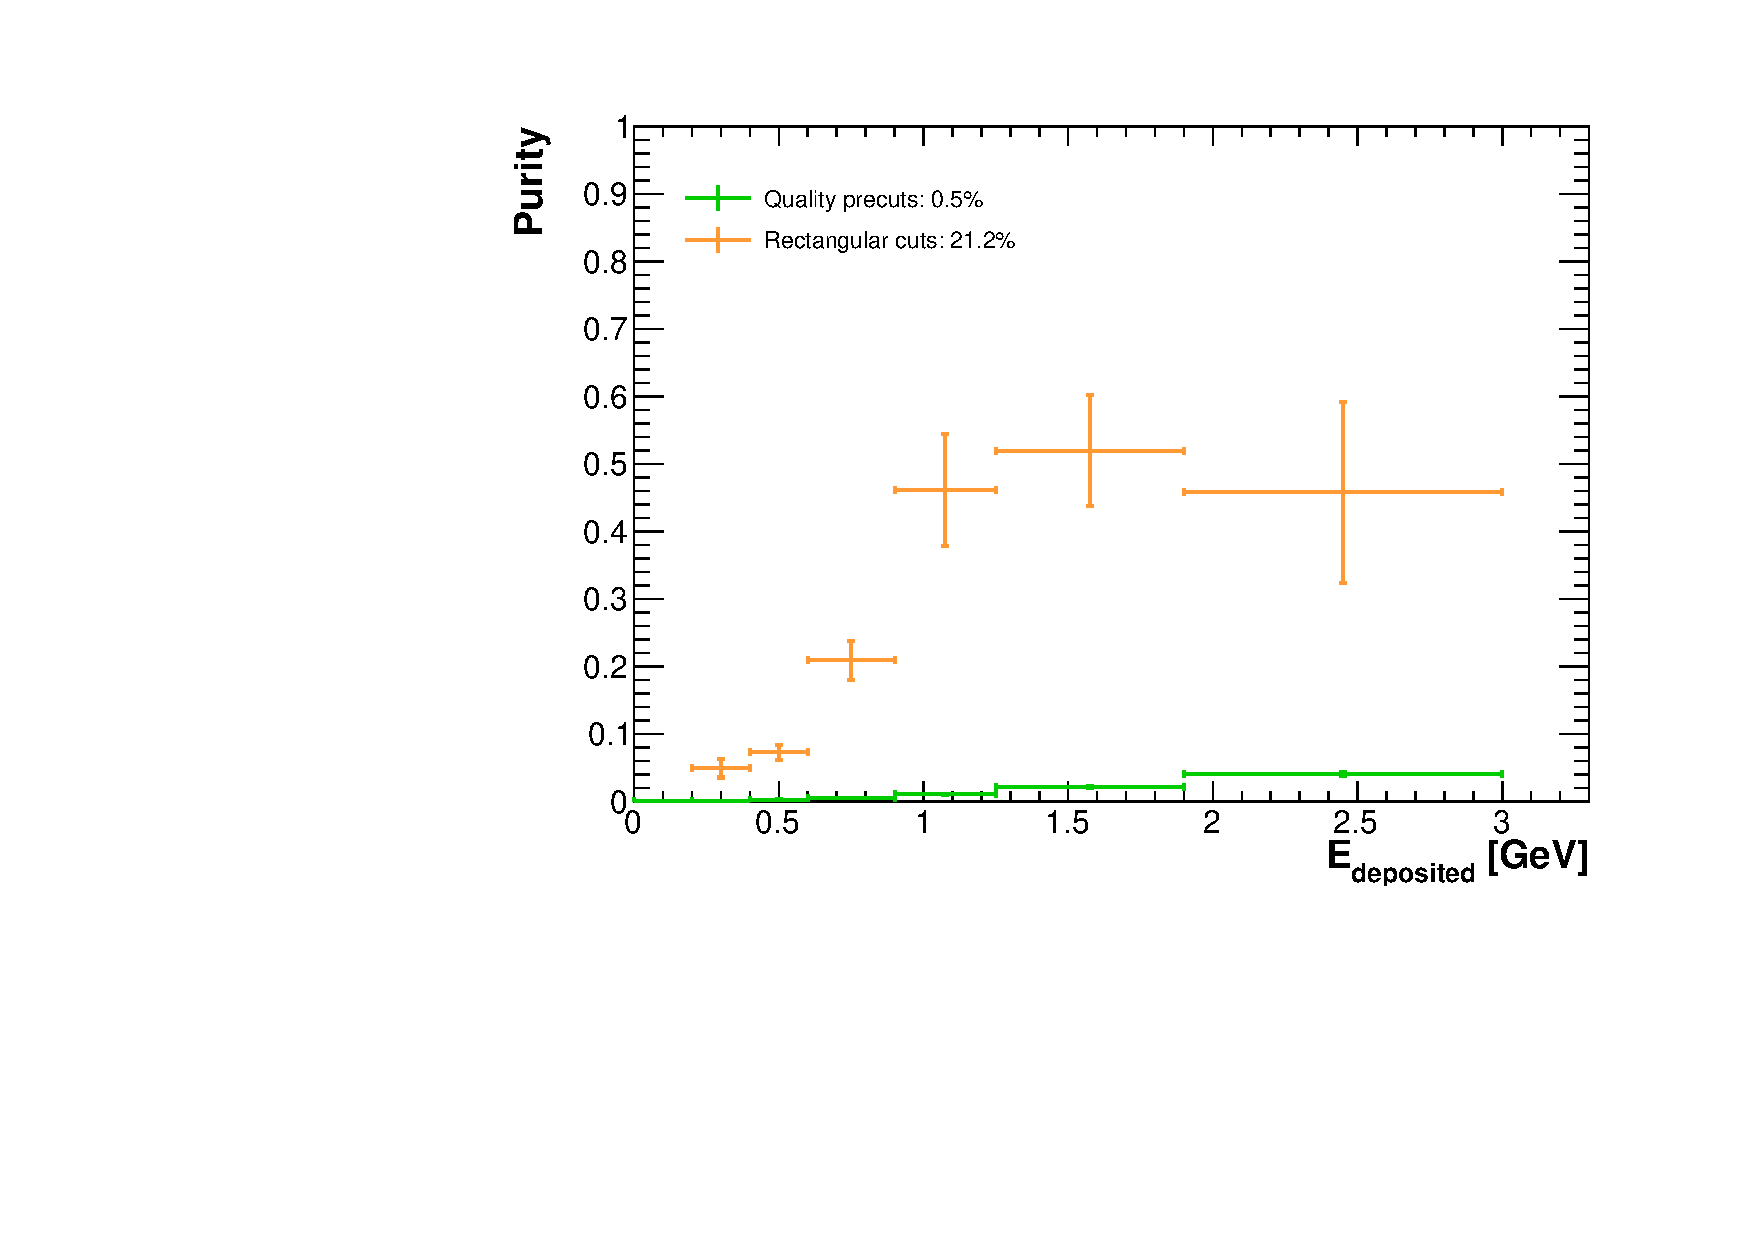
\includegraphics[width=0.75\linewidth]{figures/purity_sel.pdf}
  \caption{Purity of the selected sample before (green) and after (orange) the application of the rectangular cuts as a function of the reconstructed energy $E_{\mathrm{deposited}}$. Error bars are statistical only.}\label{fig:purity_sel}
\end{figure}


Figure \ref{fig:reco_cuts} shows the reconstructed energy spectrum $E_{\mathrm{deposited}}$ after the application of the rectangular cuts. The data and simulation agree both in shape and in normalisation.

\begin{figure}[htbp]
\centering
  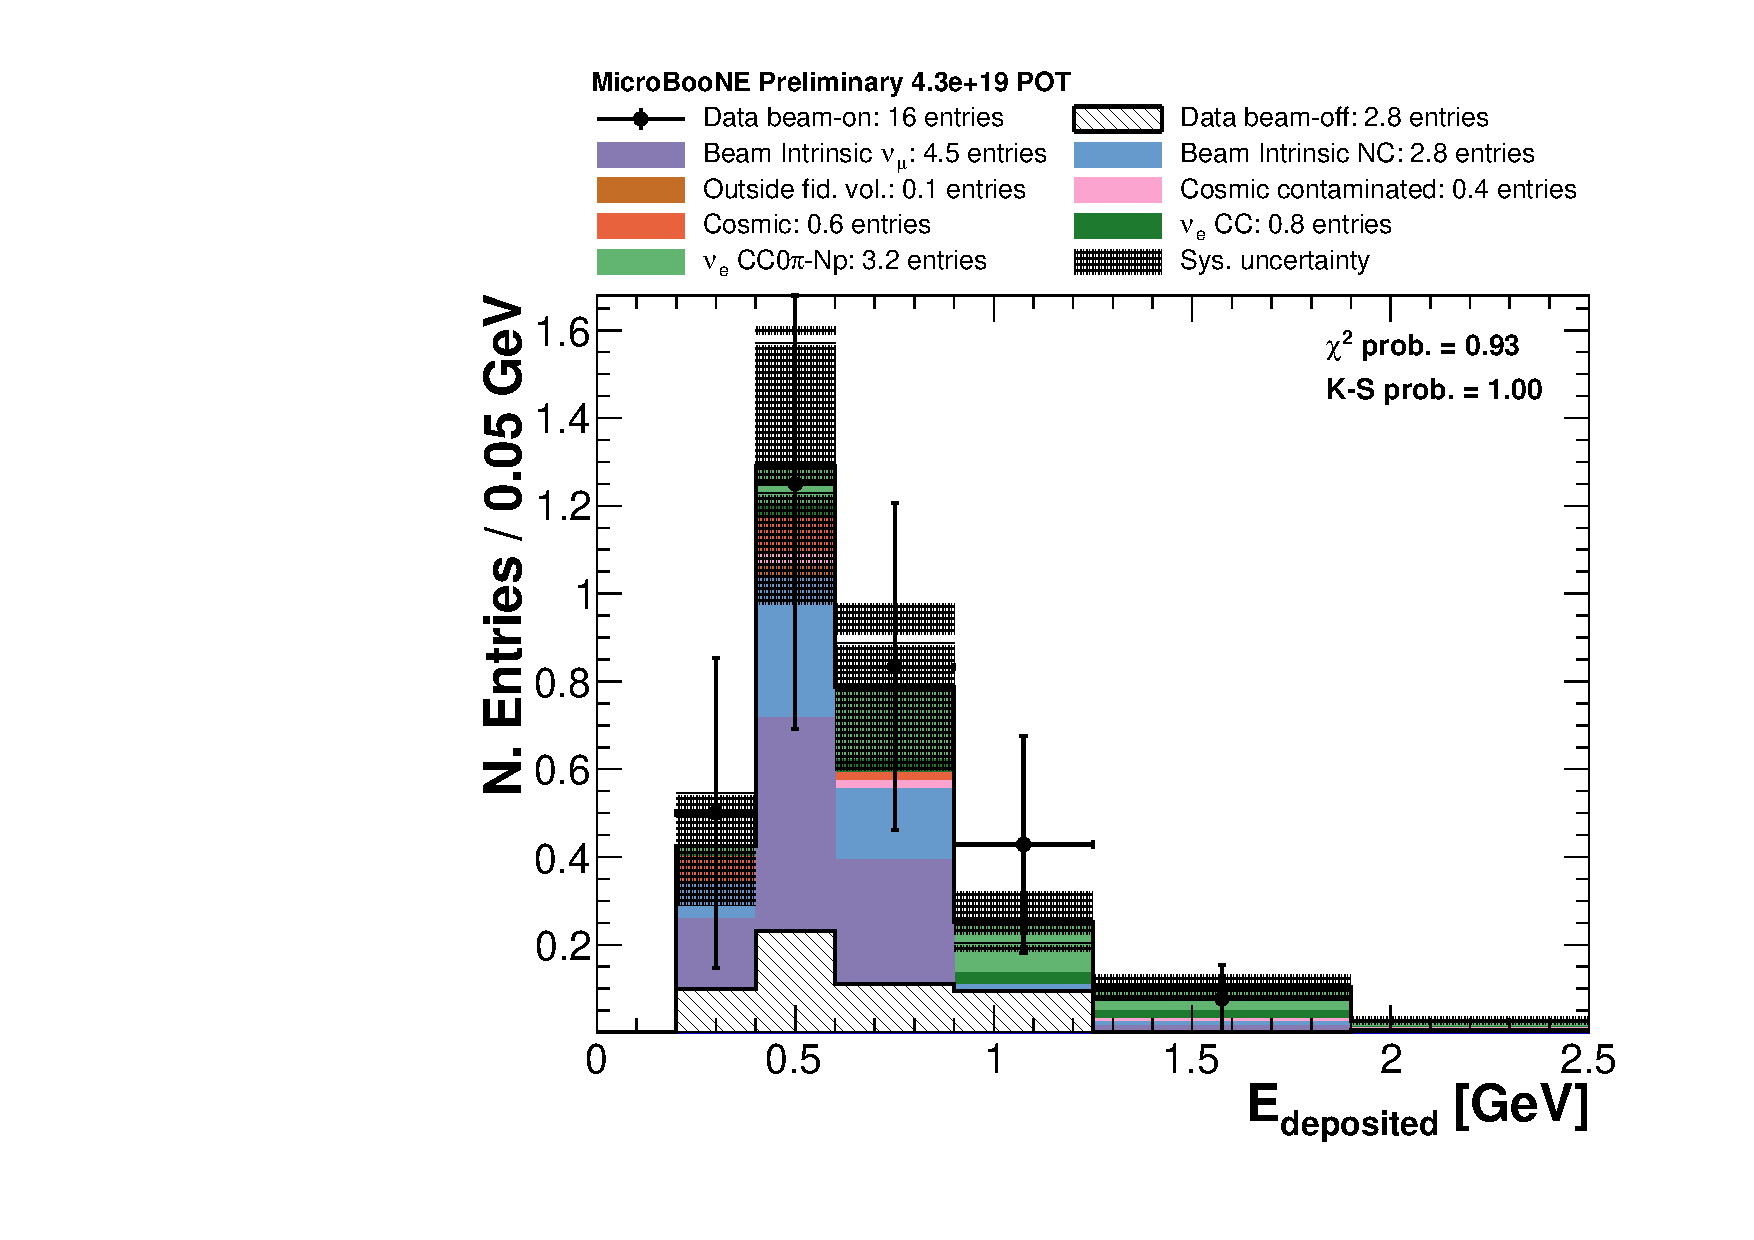
\includegraphics[width=0.75\linewidth]{figures/h_reco_energy_cuts.pdf}
  \caption{Reconstructed energy spectrum $E_{\mathrm{deposited}}$ after the application of the rectangular cuts.}\label{fig:reco_cuts}
\end{figure}

The angular distributions of the reconstructed showers are shown in Figure \ref{fig:angle_cuts}. As expected, the reconstructed showers are peaked at low values of the $\theta$ angle, since the interactions are forward-boosted, and equally distributed on the $\phi$ angle. The agreement between data and Monte Carlo is good.

\begin{figure}
\centering
  \begin{subfigure}{0.48\textwidth}
    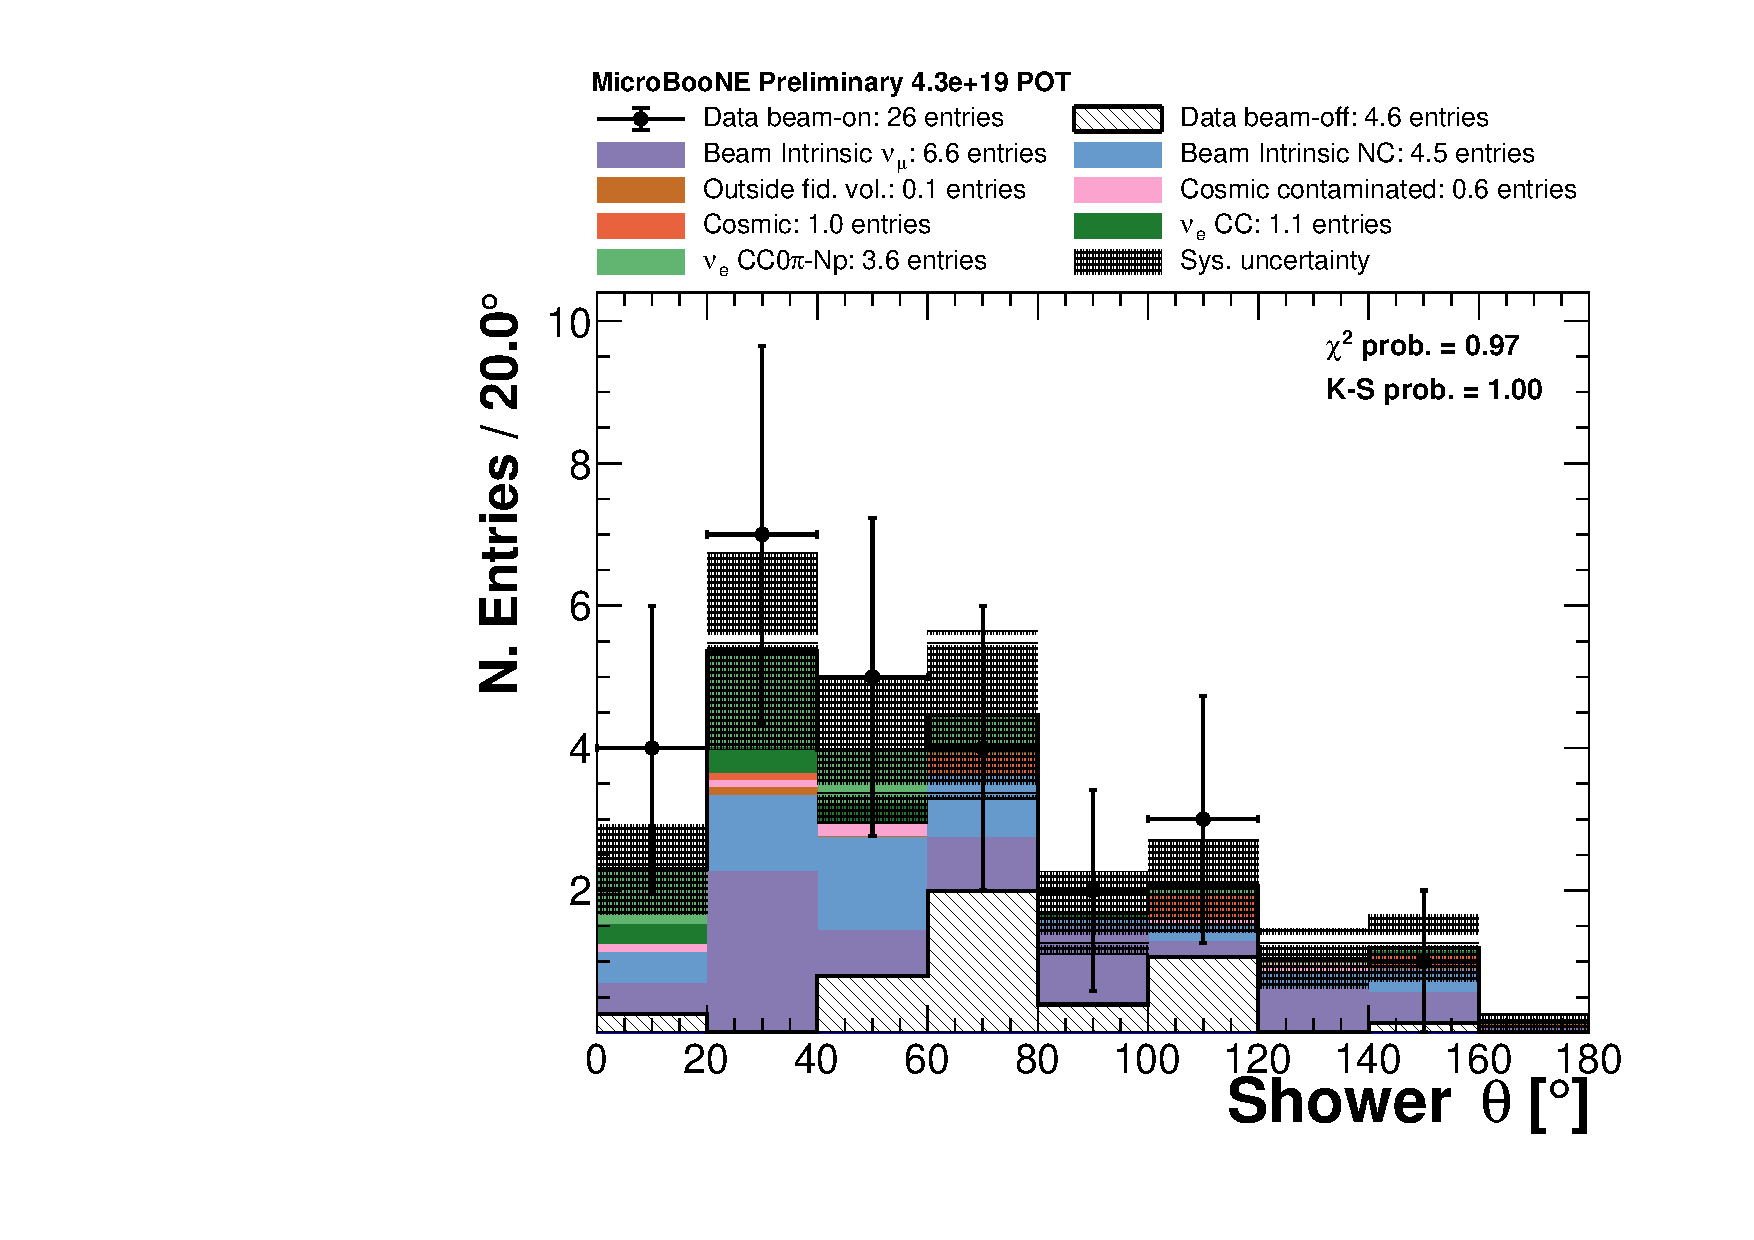
\includegraphics[width=\linewidth]{figures/theta_cuts.pdf}
    \caption{$\theta$ angle.} 
  \end{subfigure}
    \begin{subfigure}{0.48\textwidth}
    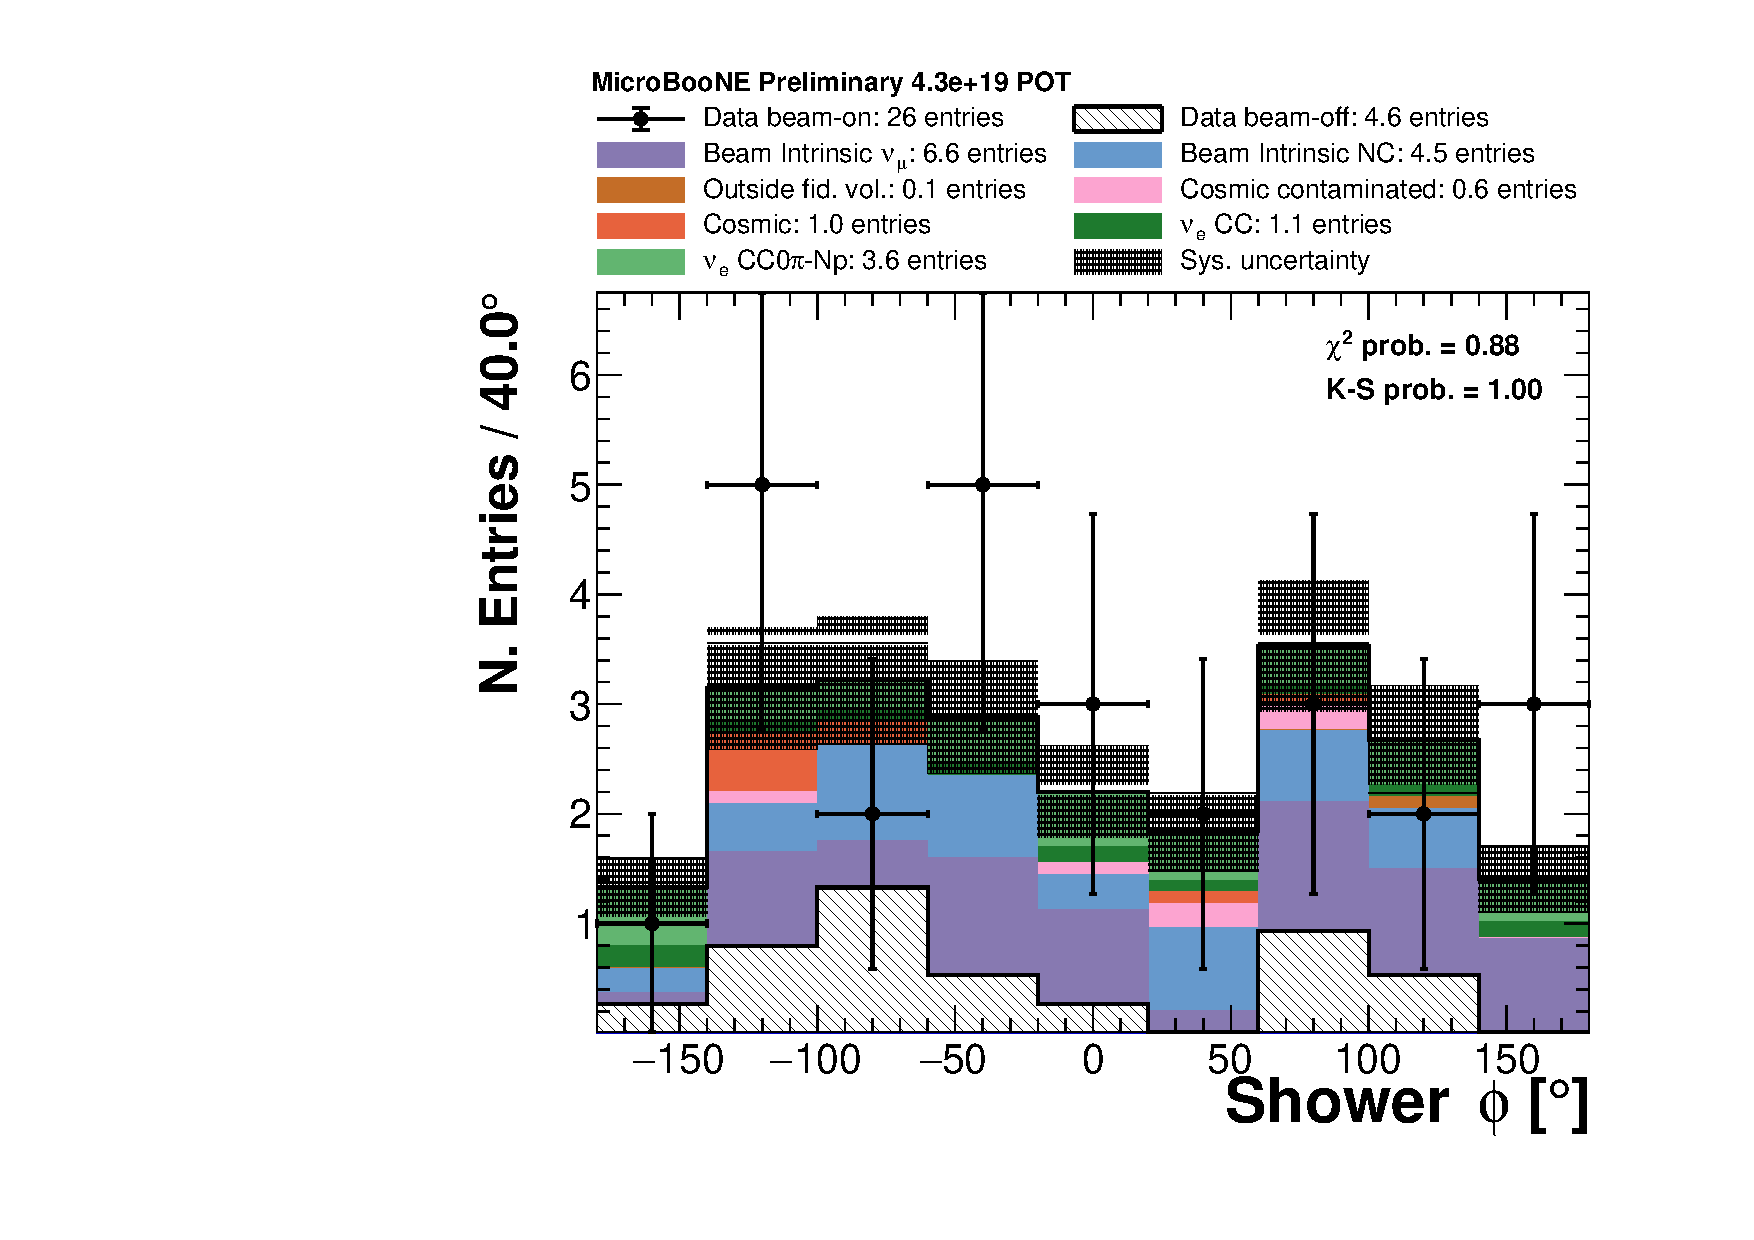
\includegraphics[width=\linewidth]{figures/phi_cuts.pdf}
    \caption{$\phi$ angle.} 
  \end{subfigure}
  \caption{Angular distribution of the selected Monte Carlo and data events after the application of the rectangular cuts.}
  \label{fig:angle_cuts}
\end{figure}

% \begin{figure}[htbp]
% \centering
%   \begin{subfigure}{0.49\textwidth}
%     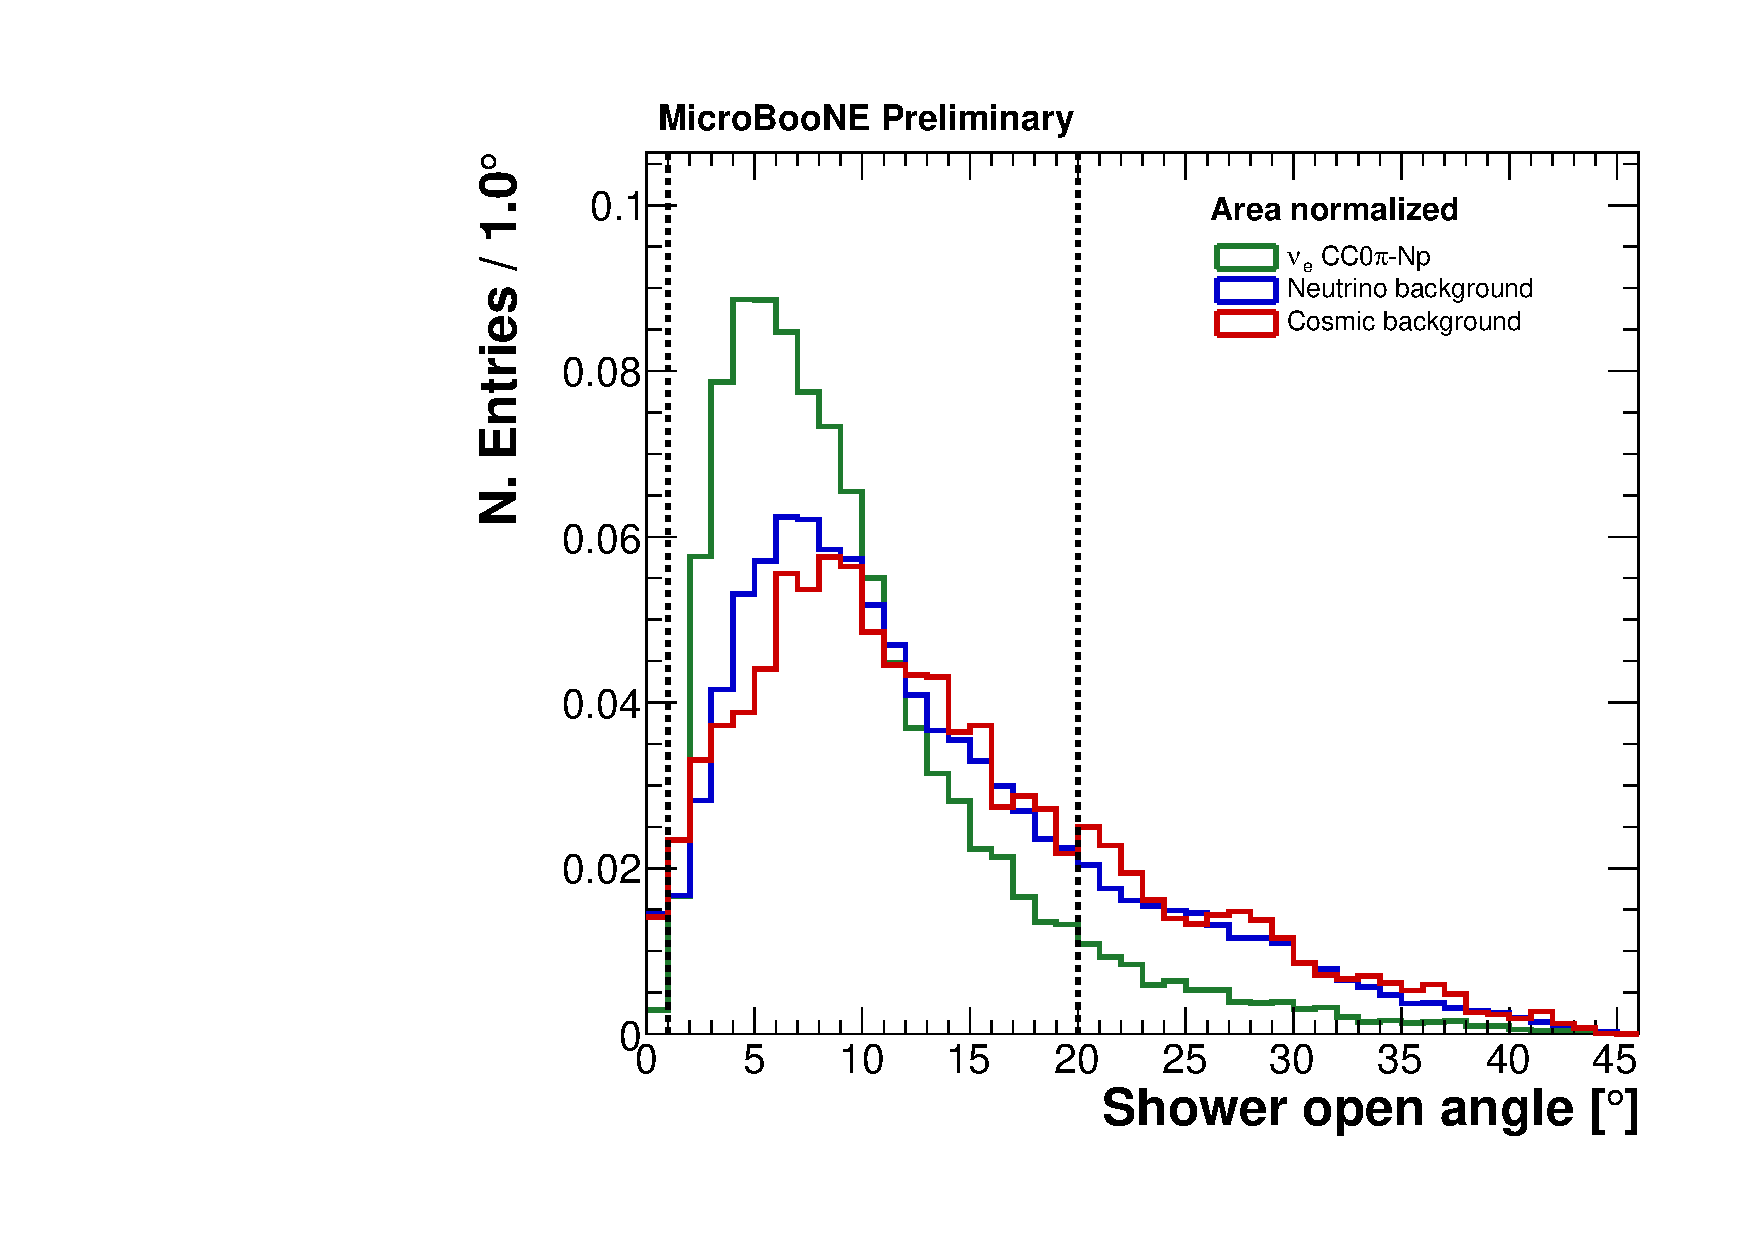
\includegraphics[width=\linewidth]{figures/h_shower_open_angle_norm.pdf}
%     \caption{Area-normalised.} \label{fig:open_norm}
%   \end{subfigure}
%     \begin{subfigure}{0.49\textwidth}
%     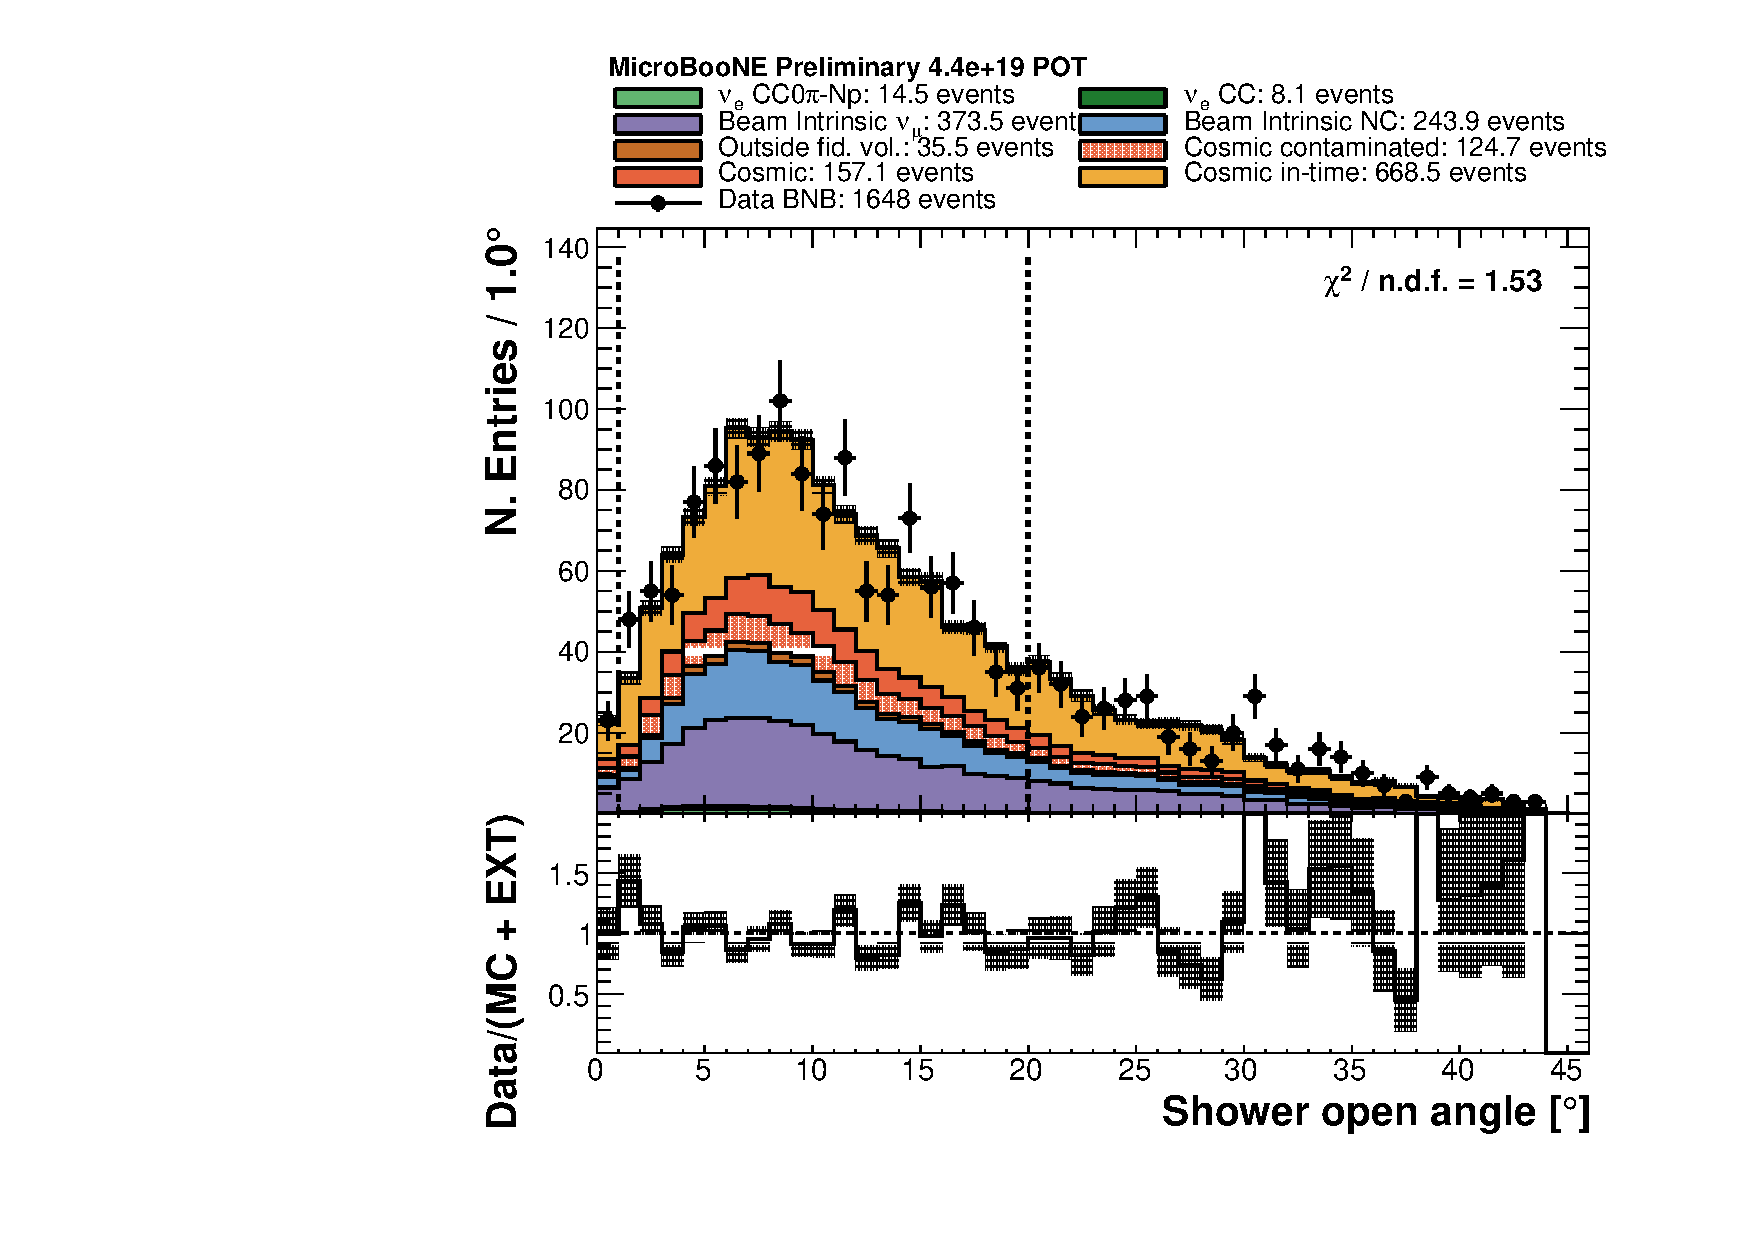
\includegraphics[width=\linewidth]{figures/h_shower_open_angle.pdf}
%     \caption{POT-normalised.} \label{fig:open_pot}
%   \end{subfigure}
%   \caption{Area and POT-normalised distributions of the opening angle $\beta$ of the most energetic shower.}
% \end{figure}


\subsection{Boosted Decision Trees}\label{sec:bdt}
\subsubsection*{Introduction}
Selecting signal events with rectangular cuts on meaningful variables allows to assess with great precision the effect of each single cut. It is therefore a very clear approach and easy to cross-check. However, it presents several limitations: many signal events may fail only a single cut and still being rejected and it is difficult to optimise the combination of a large number of cuts. 

A natural extension to the rectangular cuts approach is represented by the application of a \emph{decision tree}, widely used in social sciences and introduced recently also in high-energy physics. In particular, the MiniBooNE collaboration showed that Boosted Decision Trees (BDTs) could be used for particle identification in \cite{Yang:2005nz}, and the D0 collaboration used BDTs for the search of single top production in \cite{Abazov:2006gd}.
A classical decision tree algorithm can be divided into four stages, as listed in \cite{Coadou:2013lca}:
\begin{enumerate}
    \item sort signal and background events by each variable;
    \item select the variable and splitting value with the best separation;
    \item produce two \emph{nodes}, one containing the events passing the selection and one the events failing the selection. Each node has a defined purity, measured as the fraction of signal events in the node.
    \item repeat iteratively until the stopping condition is reached. The same variable can be used multiple times. The terminal node is called \emph{signal leaf} if it contains mostly signal events or \emph{background leaf} if it contains mostly background events.
\end{enumerate}

In this document, the separation is measured using the Gini coefficient $G$, defined as:
\begin{equation}
    G = P(1-P)\sum_i W_i,
\end{equation}
where $P$ is the purity of the node and $W_i$ is the weight of the $i$ event. The best separation is chosen as the one which minimises the $G_{\mathrm{x}}+G_{\mathrm{y}}$ sum, where $x$ and $y$ are the two new nodes of the tree.

The decision to stop the iteration can depend on multiple conditions: (1) a minimum size of the leaf can be required for statistical significance, (2) the events are perfectly classified (purity of the leaf is 1 or 0), (3) the purity cannot be improved with any choice of the splitting value, or (4) the tree depth reaches a maximum value. 
Usually, the decision tree is produced with a set of simulated events called \emph{training sample} and then applied to an independent set called \emph{test sample}.
For a single event in the test sample, the decision tree score corresponds to the purity of the leaf where the event ends up. 

The use of a decision tree to perform background rejection presents several advantages: 
\begin{itemize}
    \item it is not affected by the \emph{curse of dimensionality}: the computing consumption scales only linearly with the number of variables used;
    \item the result is insensitive to duplicate variables;
    \item the presence of very similar variables do not decrease the classification power;
    \item the order of training events is irrelevant;
    \item the result is insensitive to the transformation of the variables with any strictly monotone function (it will produce the same event ordering and, as such, the same decision tree).
\end{itemize}

A disadvantage of a classical decision tree is its intrinsic instability: a small change in the training sample can produce wildly different branches and leaves. In order to solve this problem, the so-called \emph{boosting} technique was introduced. In the boosting, training events which are misclassified (a signal event ends up in a background leaf or vice-versa) get assigned an increased weight and a new tree is formed. This process is repeated iteratively and new $m$ trees are created. The score of the individual $k$ tree $T_k$ is taken as 1 if the event ends up in a signal leaf, or -1 if the event ends up in a background leaf.  The final score $T(i)$ of the event $i$ is taken as the weighted sum of the scores of the individual trees:
\begin{equation}
    T(i) = \frac{1}{\sum^m_{k=1} \alpha_k} \sum^m_{k=1}\alpha_k T_k(i).
\end{equation}
In this document, we will use the \emph{adaptive boosting}, or AdaBoost. In this algorithm, the $\alpha$ coefficient is defined as:
\begin{equation}
    \alpha = \beta \log[(1-\epsilon)/\epsilon],
\end{equation}
where $\epsilon$ is the weighted sum of the misclassified events and $\beta$ is constant (in our case is set at 0.5). The events in the $k$ tree have their weight multiplied by $e^{a_k}$.

\subsubsection{Background rejection with Boosted Decision Trees}
In order to maximise our separation power, in this analysis we trained three different BDTs, each one tuned on a different background category:
\begin{description}
\item[Cosmic BDT:] trained with \emph{Cosmic}, \emph{Cosmic contaminated} and \emph{Data beam-off} events as background and \emph{$\nu_e$ CC0$\pi$-Np} events as signal. 
\item[Neutral-current BDT:] trained with \emph{Beam intrinsic NC} events as background and \emph{$\nu_e$~CC0$\pi$-Np} events as signal. 
\item[CC $\nu_{\mu}$ BDT:] trained with \emph{Beam intrinsic $\nu_{\mu}$} events as background and \emph{$\nu_e$~CC0$\pi$-Np} events as signal. 
\end{description}

The variables used are the same in all three BDTs and they correspond to the ones described in Section \ref{sec:cuts}. The BDT has been trained on 600 trees, using the Gini coefficient to measure the splitting power, requiring at least 5\% of the training events in each terminal node, and using the AdaBoost boosting algorithm. The training has been performed with the TMVA toolkit \cite{Hocker:2007ht}. 

The classification power of the BDTs can be compared by looking at the Receiver Operating Characteristic (ROC) curves, which shows the background-rejection power as a function of the signal efficiency. Figure \ref{fig:roc} shows the ROC curves for our three BDTs, in the case of samples with 1000 signal events and 1000 background events. The best-performing BDT is the \emph{Cosmic BDT}. This is expected, since cosmic rays have greatly different angular, topological, and kinematic distributions when compared with neutrino interactions. 

\begin{figure}[htbp]
\centering
  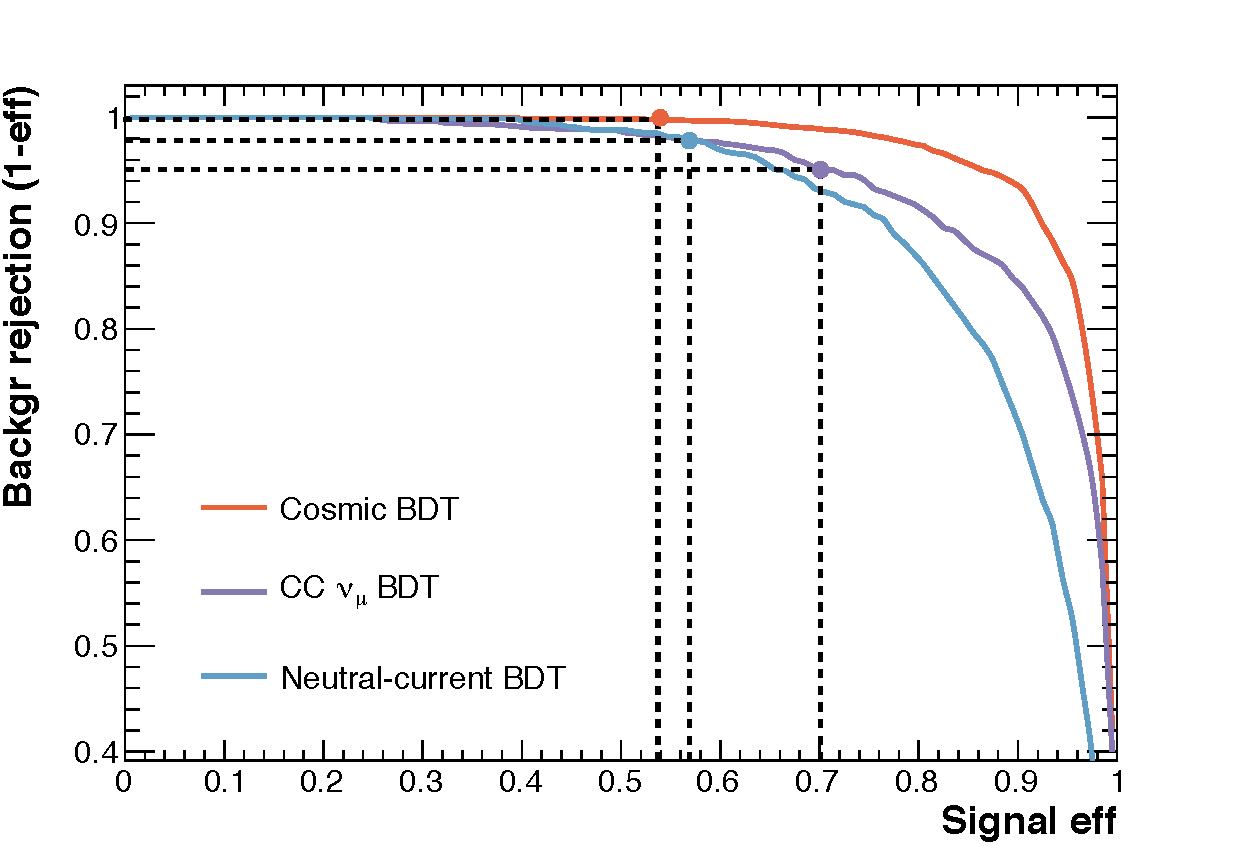
\includegraphics[width=0.75\linewidth]{figures/roc.pdf}
  \caption{ROC curves for the three BDTs used in this analysis, showing the background-rejection power as a function of the signal efficiency in a sample with 100 signal events and 1000 background events.}\label{fig:roc}
\end{figure}

The least powerful BDT is the \emph{Neutral current BDT}. This is because NC events with $\pi^0$ production are the most difficult events to reject. As we have seen in Section \ref{sec:dedx}, photons which undergo very asymmetric pair-production can have a $dE/dx$ around $2$~MeV. When one of the photons of the $\pi^0\rightarrow\gamma\gamma$ decay escapes the detector or is not reconstructed, and the other one pair-produces asymmetrically near the interaction vertex, the event become basically indistinguishable from a $\nu_e$~CC0$\pi$-Np interaction.

The BDT is then applied to an independent Monte Carlo sample (the \emph{test sample}) and to our data. It is very important to verify the agreement between the BDTs score distribution in data and Monte Carlo, since the presence of a bias in our training could create a fake excess.

Figure \ref{fig:bdt_datamc} shows the comparison between the data and Monte Carlo distributions for the Cosmic, Neutral-current, and CC $\nu_{\mu}$ BDTs. 

\begin{figure}[htbp]
\centering
  \begin{subfigure}{0.32\textwidth}
    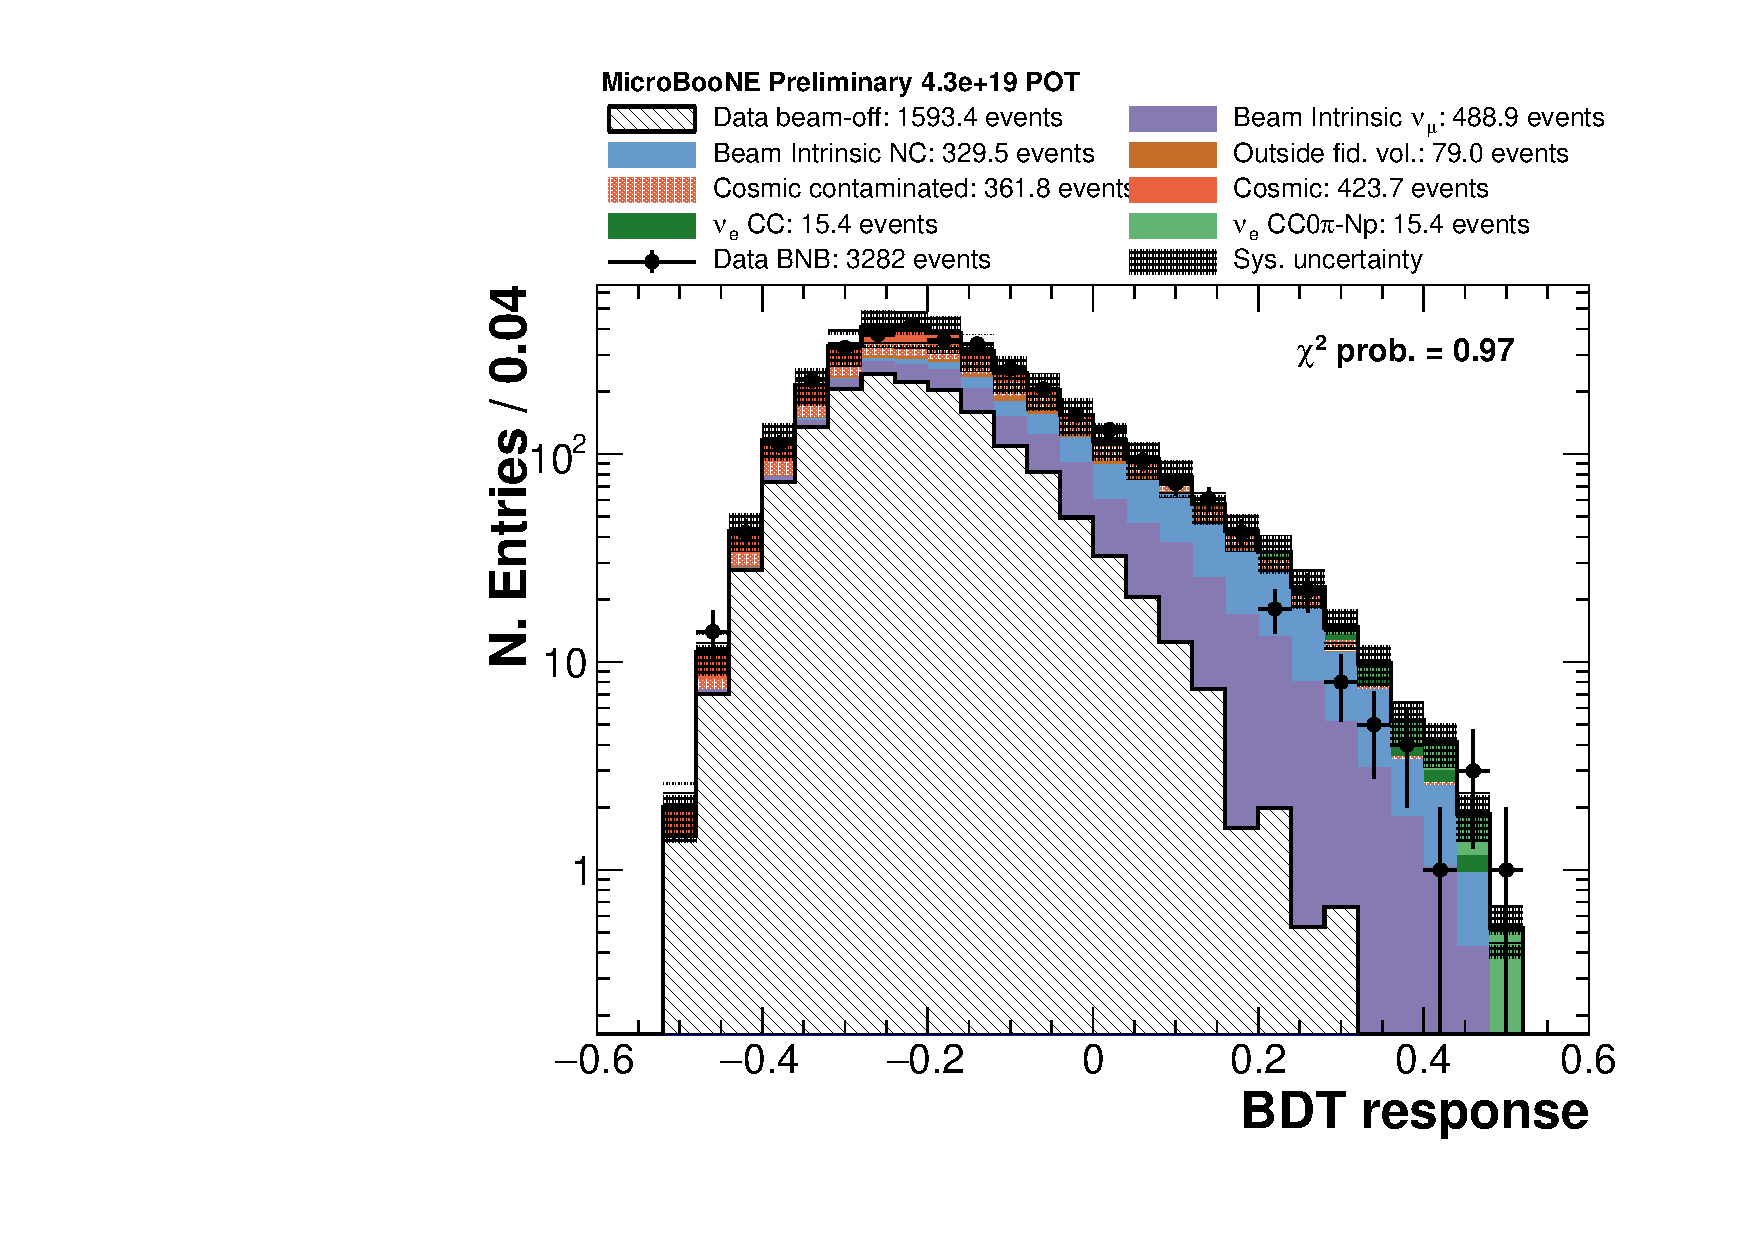
\includegraphics[width=\linewidth]{figures/bdt_cosmic.pdf}
    \caption{Cosmic} 
  \end{subfigure}\begin{subfigure}{0.32\textwidth}
    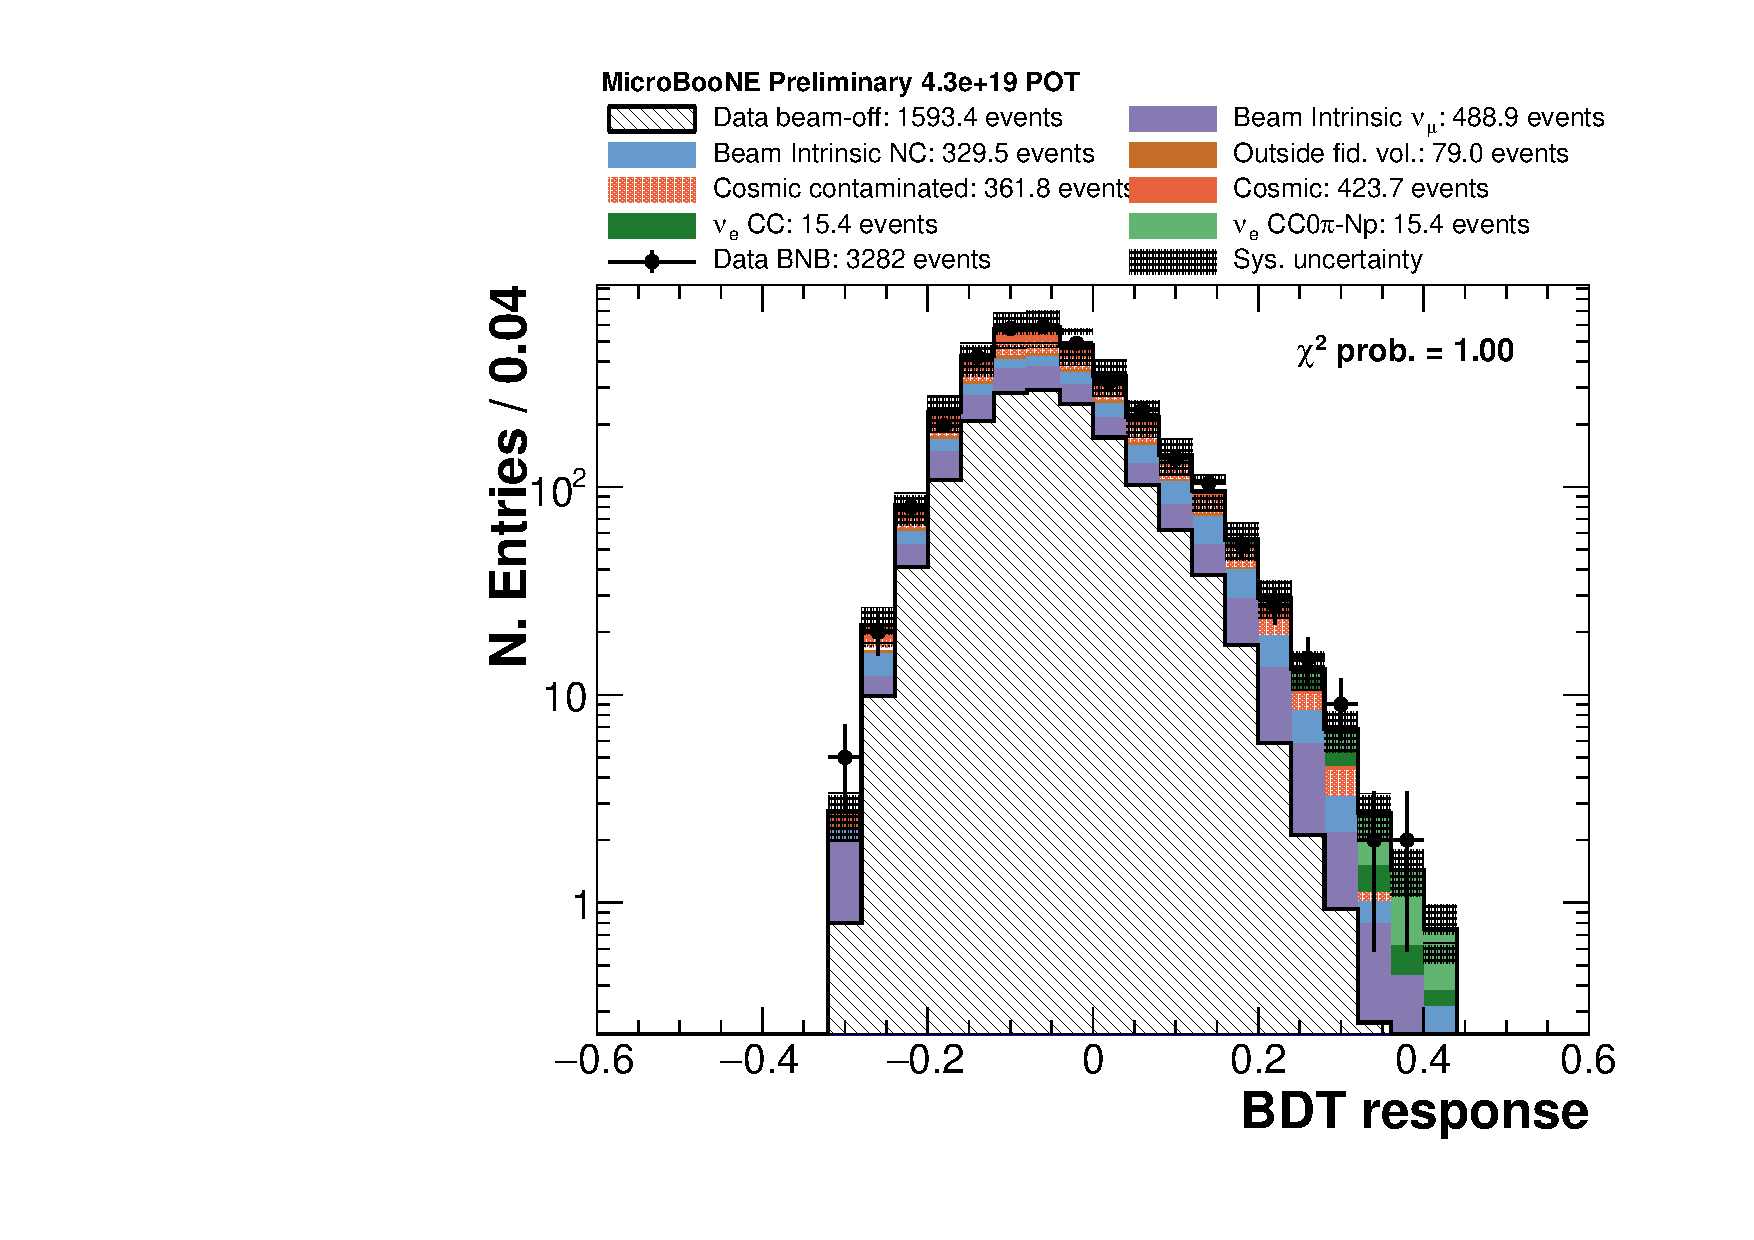
\includegraphics[width=\linewidth]{figures/bdt_nc.pdf}
    \caption{Neutral-current}
  \end{subfigure}\begin{subfigure}{0.32\textwidth}
    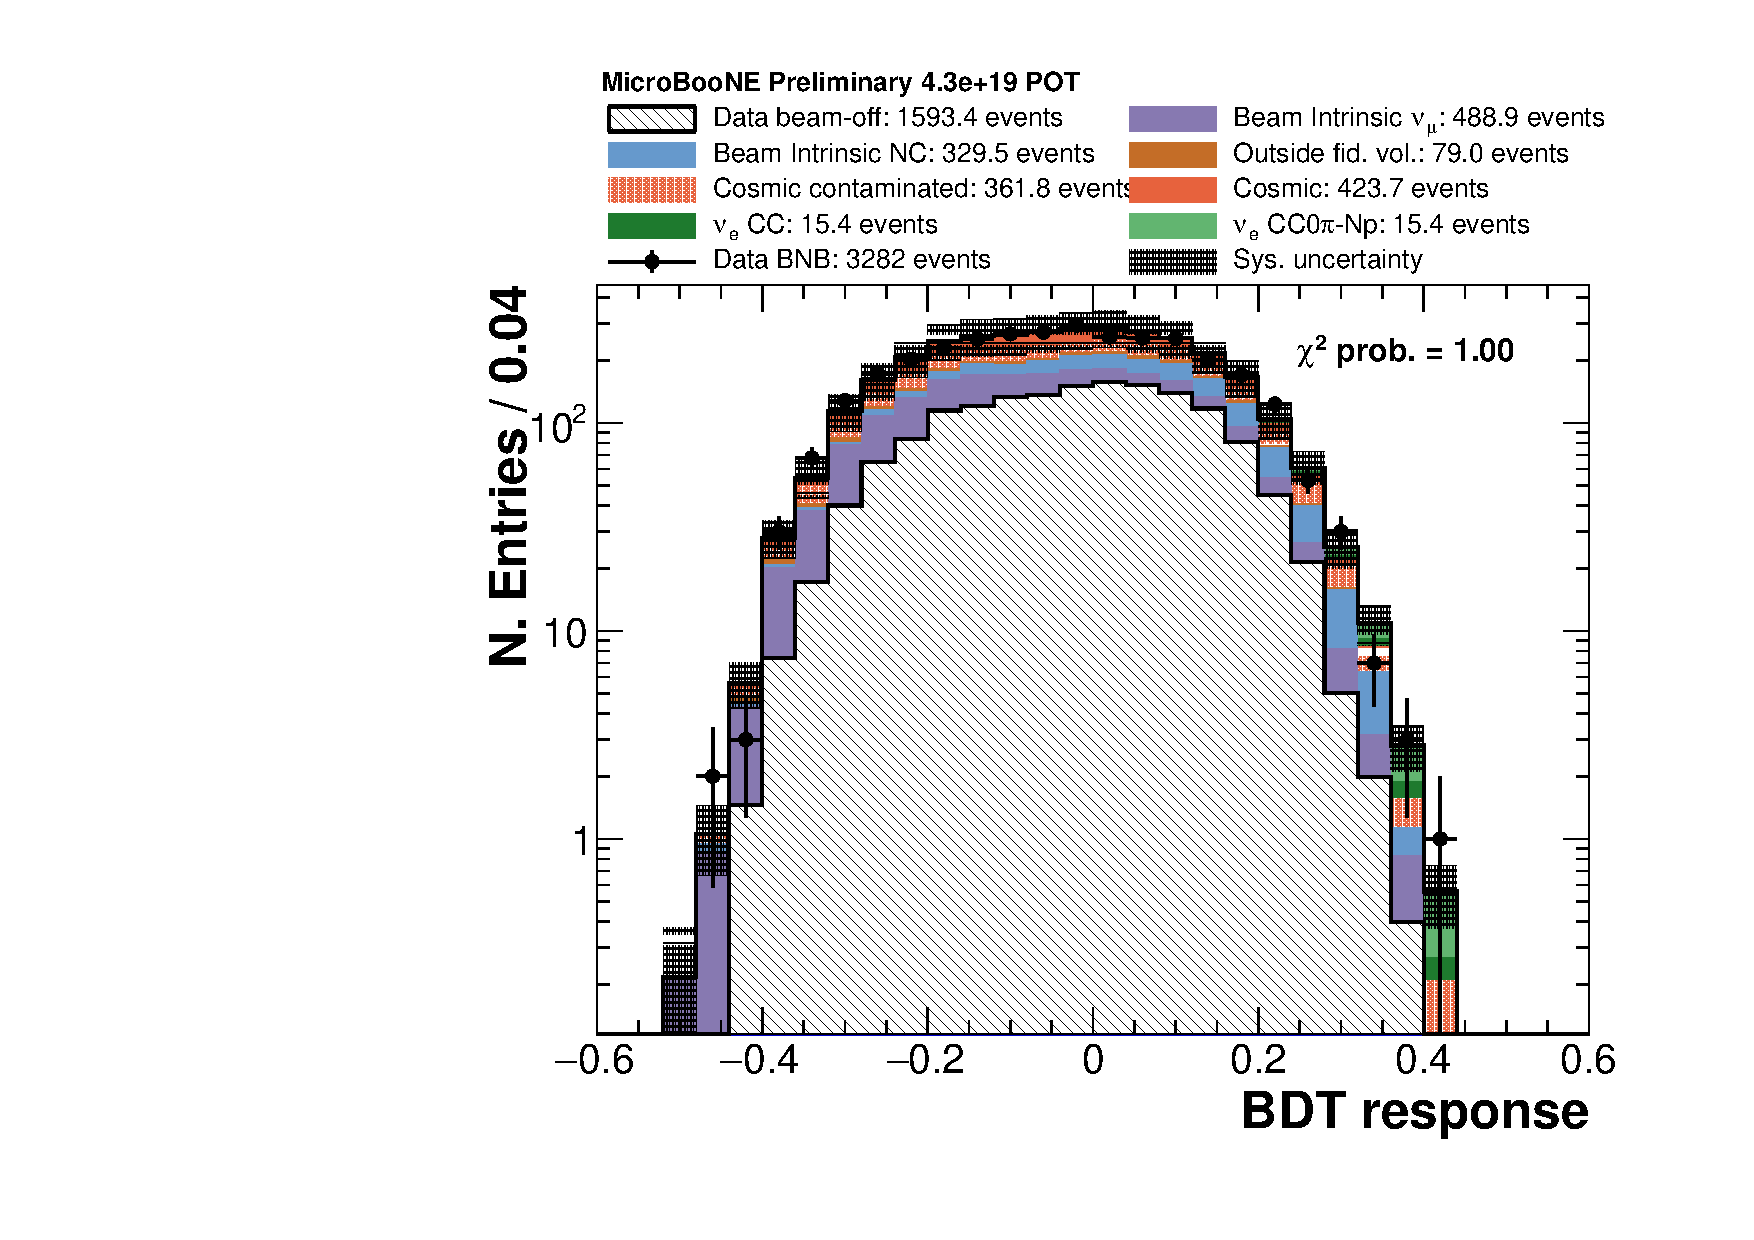
\includegraphics[width=\linewidth]{figures/bdt_numu.pdf}
    \caption{CC $\nu_{\mu}$} 
  \end{subfigure}
  \caption{POT-normalised comparison between the data and Monte Carlo for distributions of the BDTs score.}\label{fig:bdt_datamc}
\end{figure}

In order to maximise our $\nu_e$ CC0$\pi$-Np purity and at least one event per bin in the $[0.2,1.9]$~GeV range of the $E_{\mathrm{deposited}}$ spectrum (same criterion used for the rectangular cuts), we applied the following cuts:
\begin{equation}
    \text{Cosmic BDT} > 0.21,~~~\text{Neutral-current BDT} > 0.18,~~~\text{CC }\nu_{\mu}\text{ BDT} > 0.17.
\end{equation}

We select 14 data beam-on events, 0.5 beam-off events, and 9.5 Monte Carlo events. The number of selected $\nu_e$ CC0$\pi$-Np events is $4.4$, which corresponds to a final efficiency of $(13.0\pm0.3~\mathrm{(stat)}\pm0.5~\text{(sys)})\%$. The final purity of the sample is $44.3\%$, around twice the one obtained with the rectangular cuts (Figure \ref{fig:purity_bdt}).

\begin{figure}[htbp]
\centering
  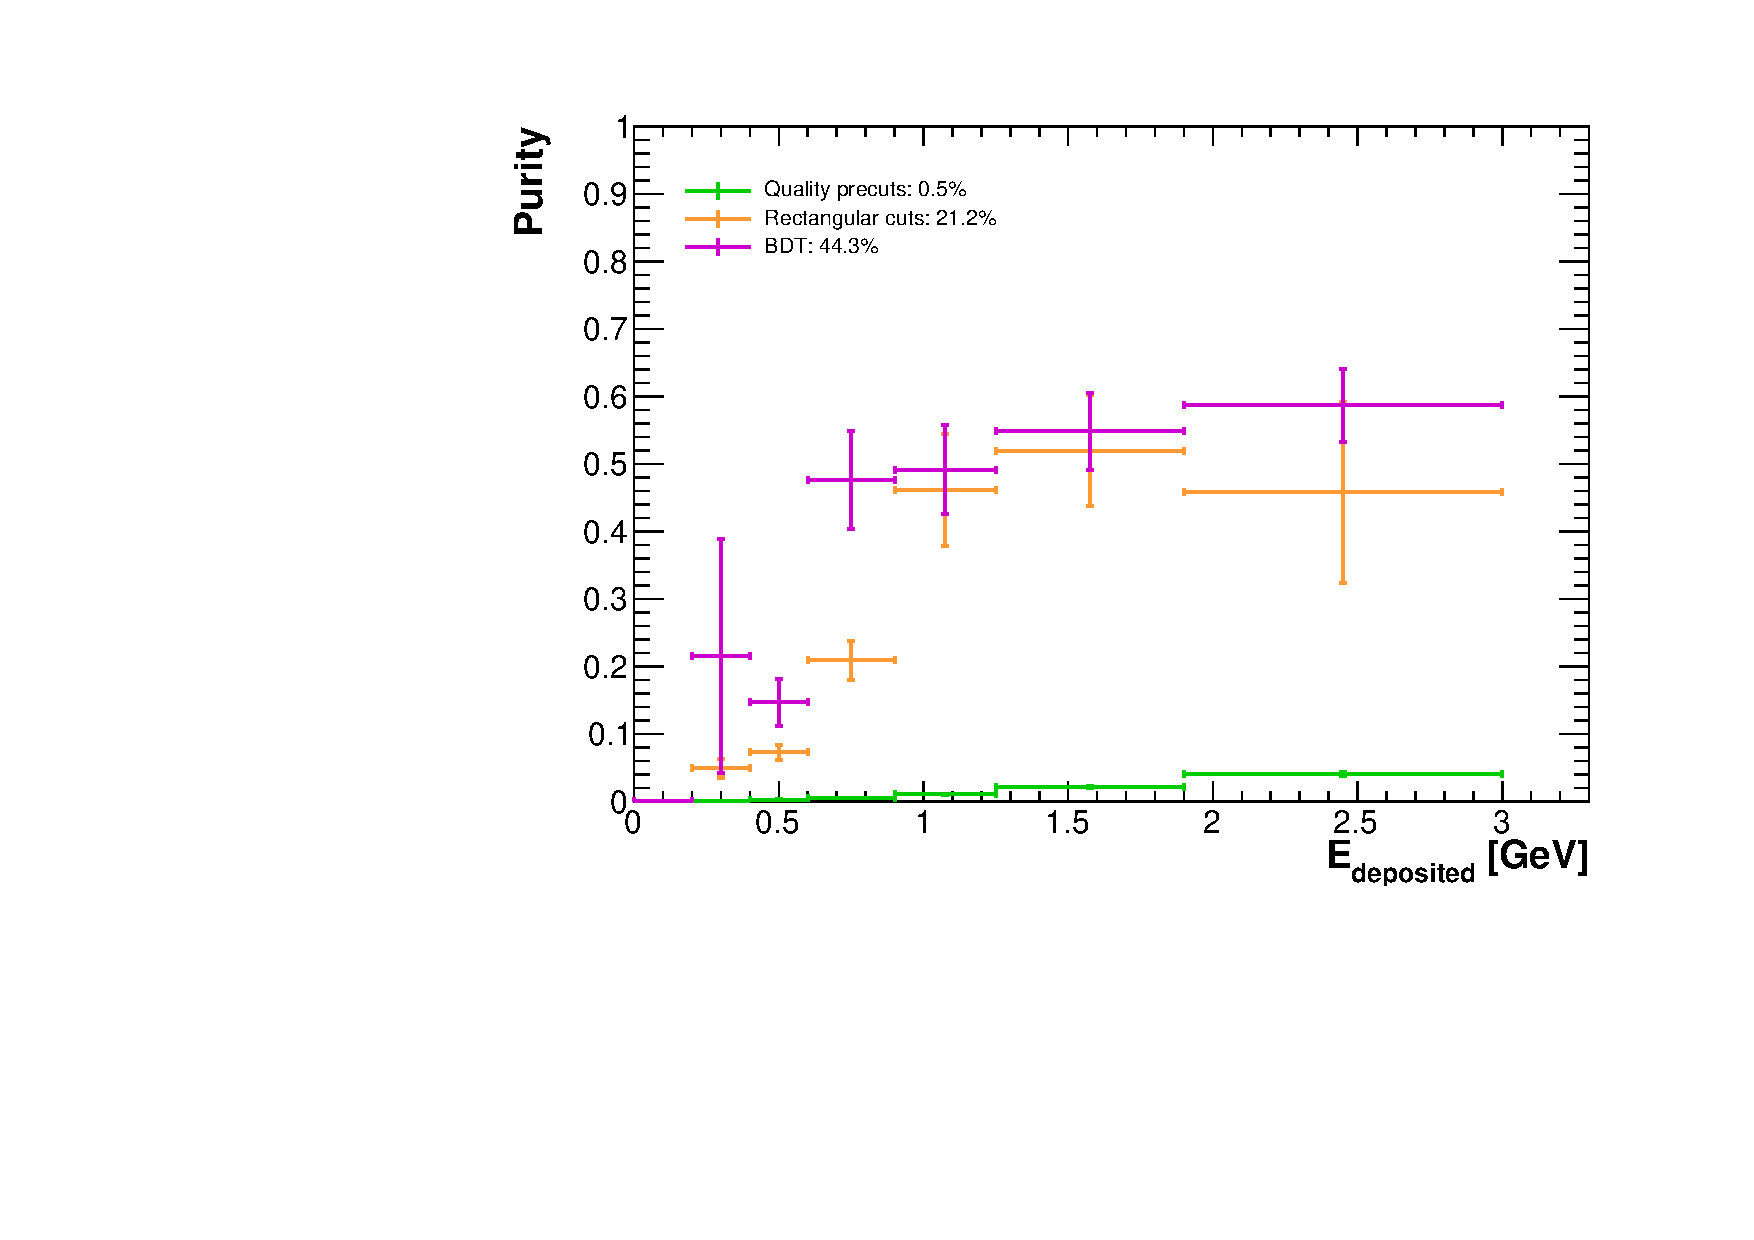
\includegraphics[width=0.75\linewidth]{figures/purity_bdt.pdf}
  \caption{Purity of the sample after the event selection (green), after the application of the rectangular cuts (orange), and after the application of the BDTs (purple) as a function of the reconstructed energy $E_{\mathrm{deposited}}$. Error bars are statistical only.}\label{fig:purity_bdt}
\end{figure}

The distribution of the reconstructed energy spectrum $E_{\mathrm{deposited}}$ after the application of the three BDT cuts is shown in Figure \ref{fig:reco_bdt}. 

\begin{figure}[htbp]
\centering
  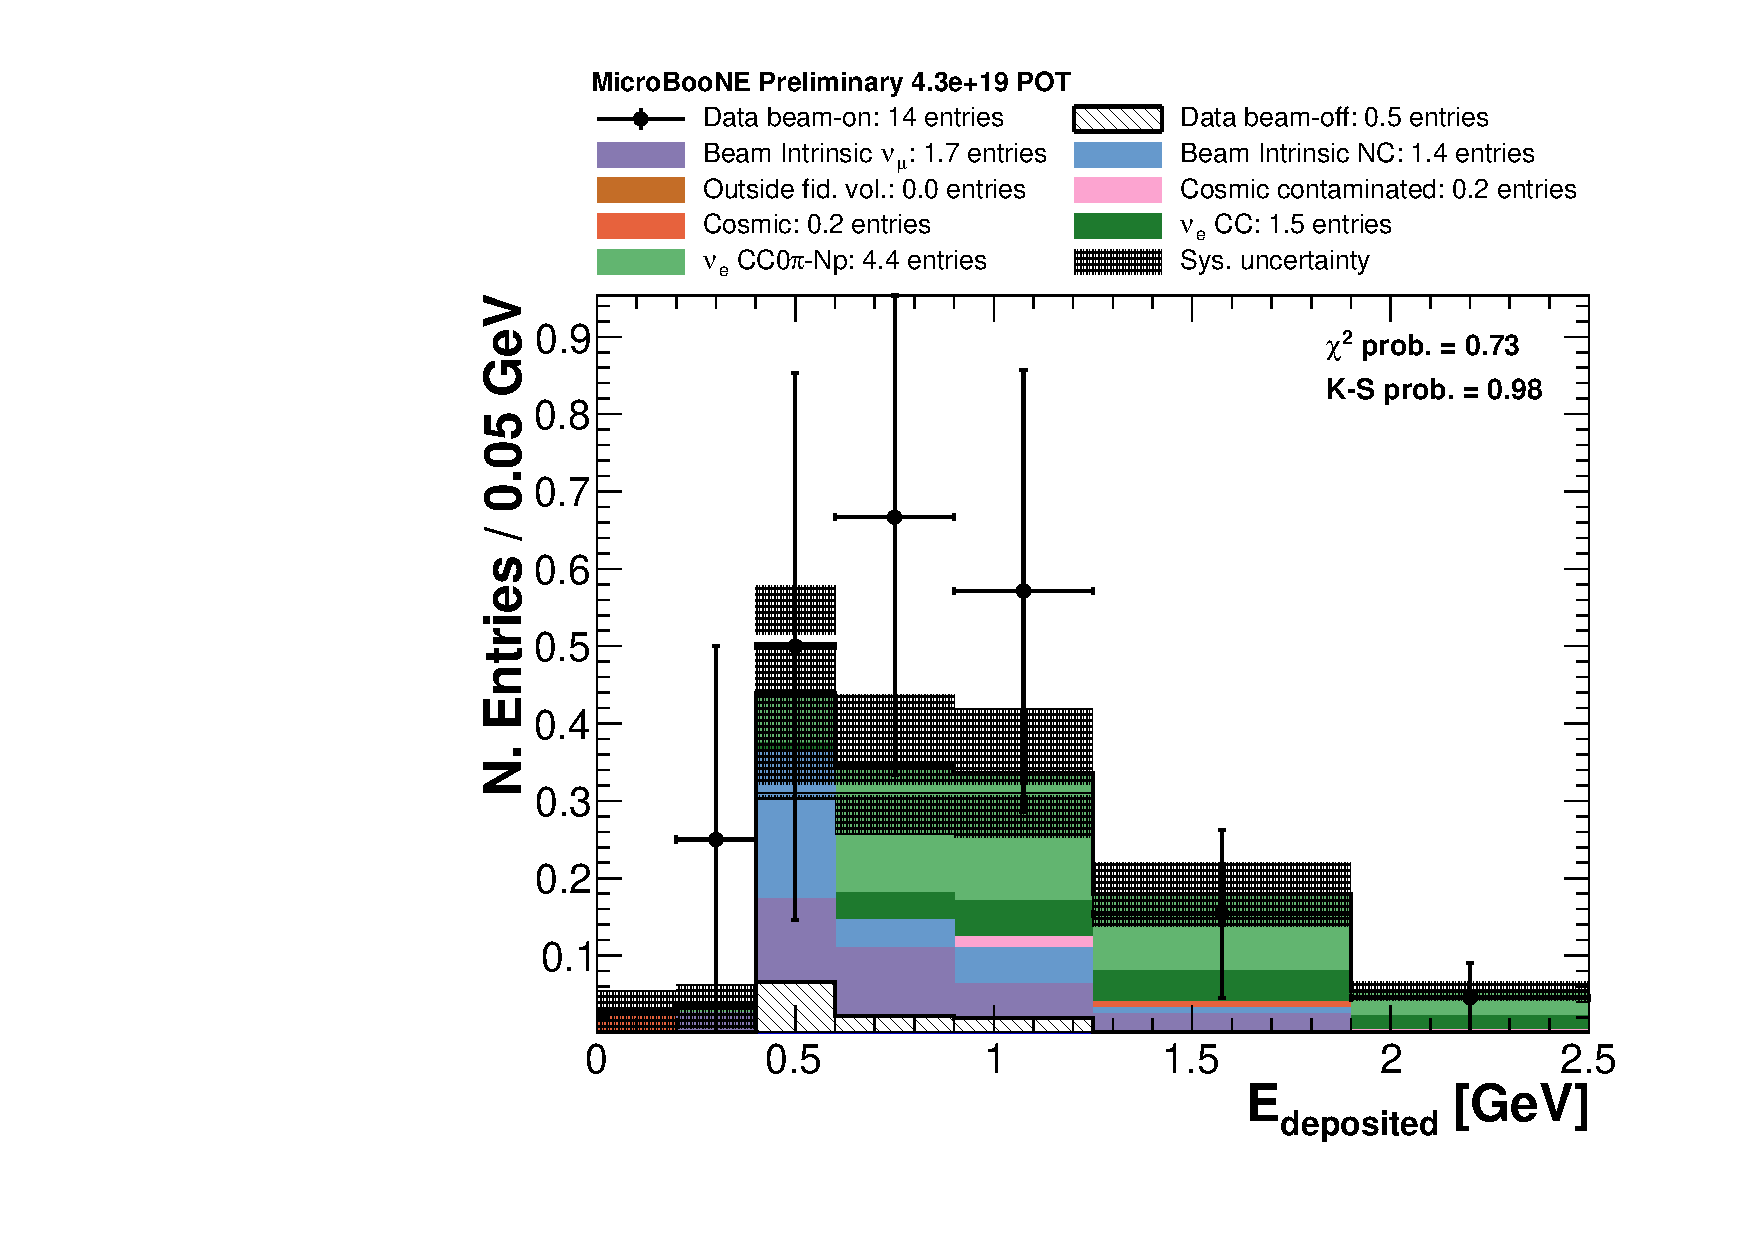
\includegraphics[width=0.75\linewidth]{figures/h_reco_energy_bdt.pdf}
  \caption{Reconstructed energy spectrum $E_{\mathrm{deposited}}$ after the application of the BDTs cuts.}\label{fig:reco_bdt}
\end{figure}

The angular distributions of the reconstructed showers are shown in Figure \ref{fig:angle_bdt}. 

\begin{figure}
\centering
  \begin{subfigure}{0.48\textwidth}
    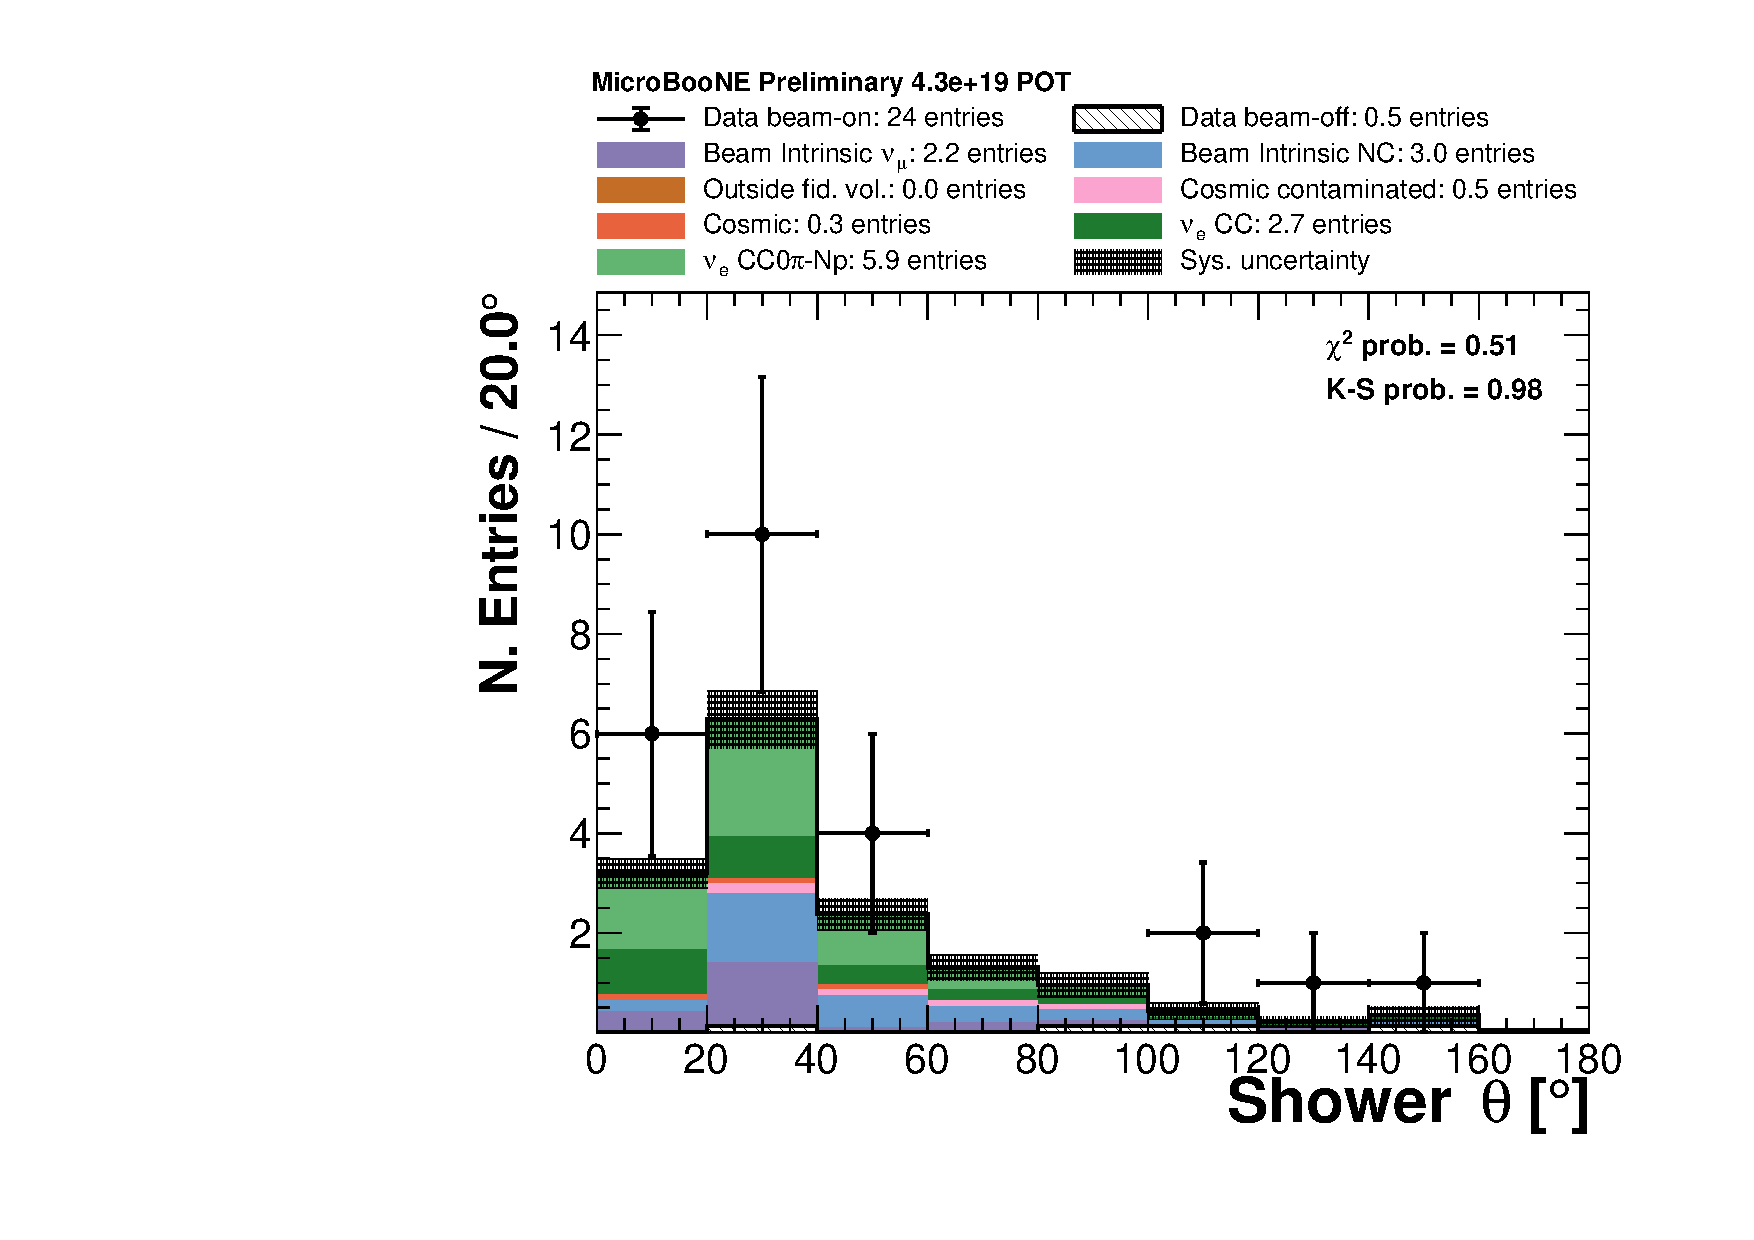
\includegraphics[width=\linewidth]{figures/theta_bdt.pdf}
    \caption{$\theta$ angle.} 
  \end{subfigure}
    \begin{subfigure}{0.48\textwidth}
    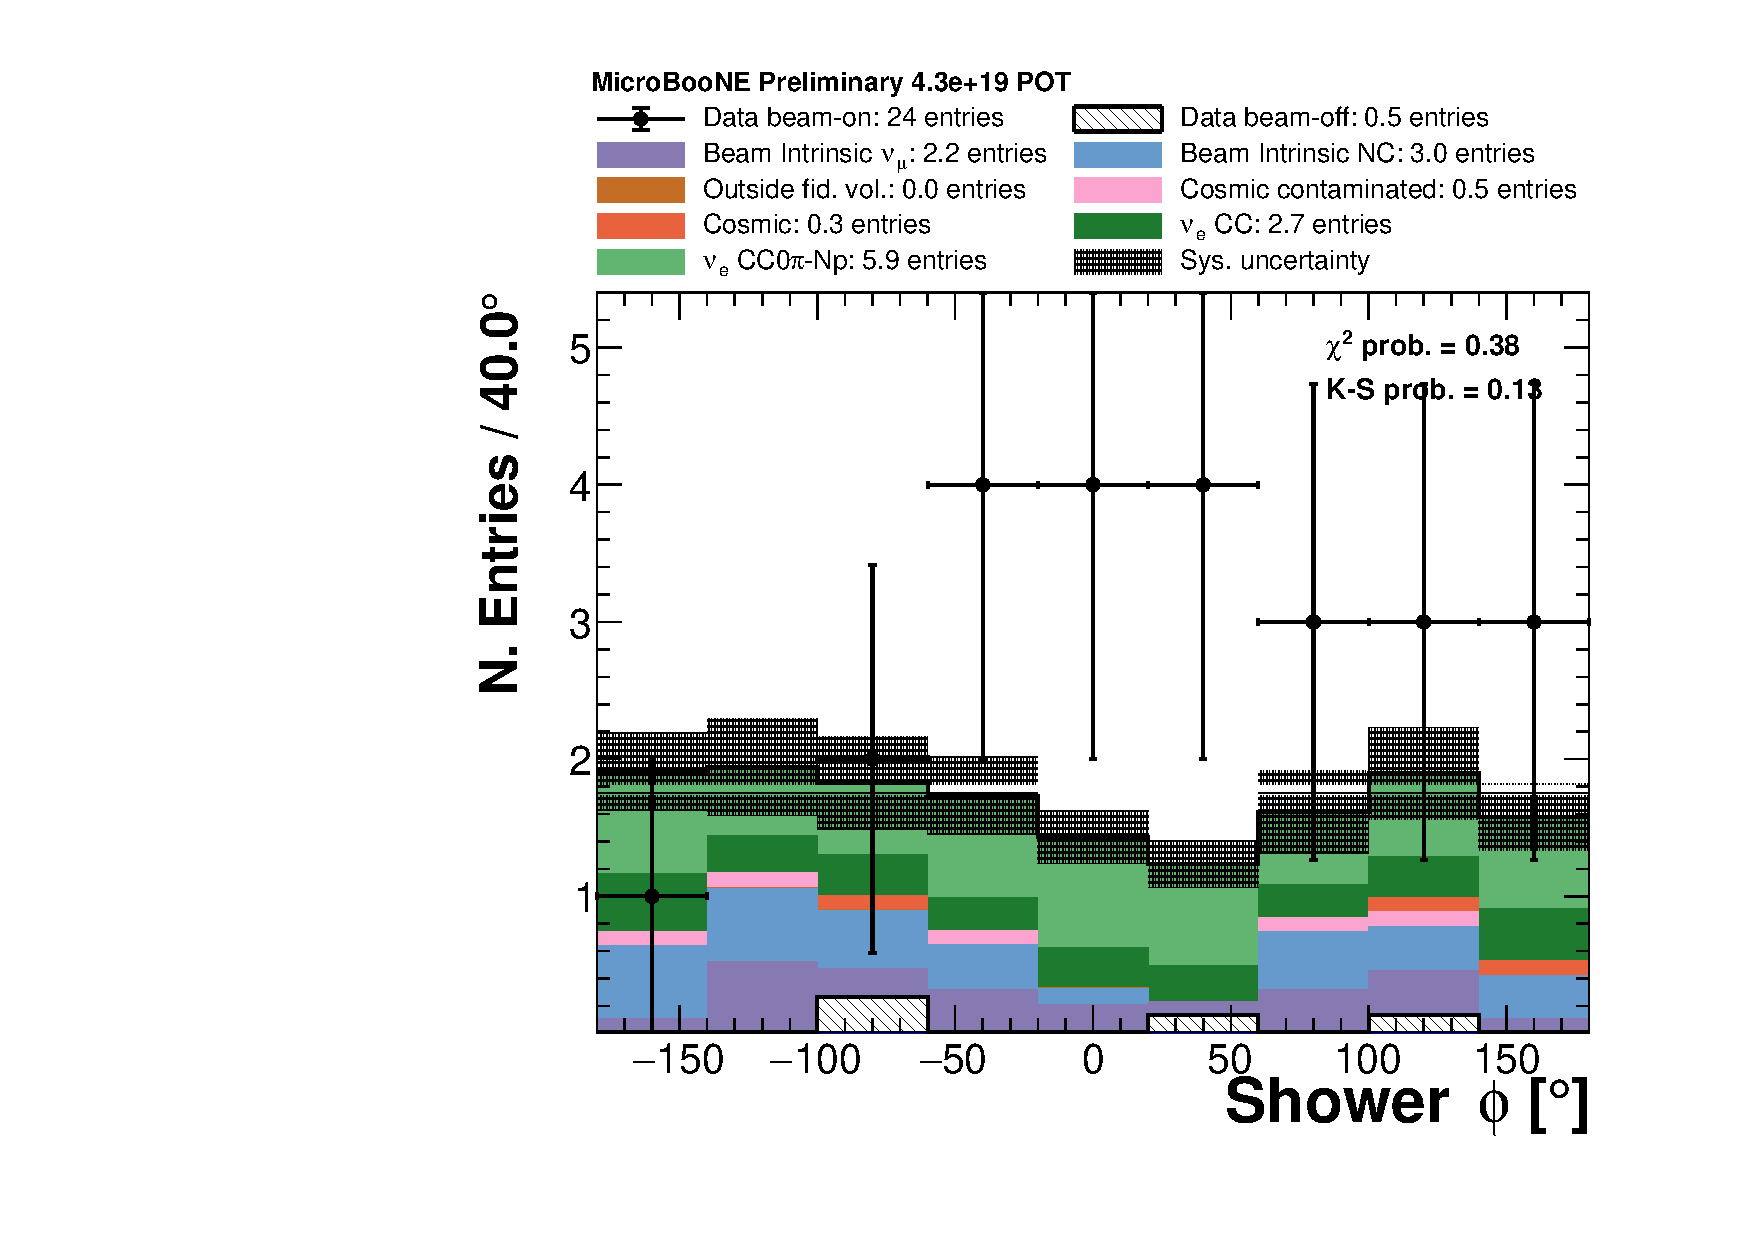
\includegraphics[width=\linewidth]{figures/phi_bdt.pdf}
    \caption{$\phi$ angle.} 
  \end{subfigure}
  \caption{Angular distribution of the selected Monte Carlo and data events after the application of the BDTs cuts.}
  \label{fig:angle_bdt}
\end{figure}